% -*-coding: utf-8;-*-
%%%%%%%%%%%%%%%%%%%%%%%%%%%%%%%%%%%%%%%%%%%%%%%%%%%%%%%%%%%%%%%%%%%%%%%%%%%%%%
% Главный файл
\documentclass[12pt]{rusthesis}
% do not use [draft] otherwise all PS graphics will disappear
\usepackage[T2A]{fontenc}
\usepackage[utf8]{inputenc}
\usepackage{graphicx}
\usepackage{latexcad}
\usepackage{amsmath}
\usepackage{amssymb}
\usepackage{eepic}
\usepackage{epsfig}
\usepackage{pgf}
\usepackage{tikz}
\usepackage{pstricks}
\bibliographystyle{plain}

\language=4

% My macros
\newcommand\tablref[1]{\cyrt\cyra\cyrb\cyrl.~\ref{#1}}
\newcommand\figref[1]{\cyrr\cyri\cyrs.~\ref{#1}}
\newcommand\pgref[1]{\cyrs.~\pageref{#1}}
%\newcommand\eqref[1]{(\ref{#1})}

\renewcommand{\tan}{\mathop{\rm tg}}
\renewcommand{\arctan}{\mathop{\rm arctg}}
\renewcommand{\tanh}{\mathop{\rm th}}
\newcommand{\DEF}{\mathrel{\mathop=^{\rm def}}}
\newcommand{\MSE}{\overline{\varepsilon^2}}
\newcommand{\hatMSE}{\overline{\hat{\varepsilon}^2}}
\newcommand{\MSEmin}{\overline{\varepsilon^2}_{\rm min}}
\newcommand{\dt}{\Delta t}
\newcommand{\NN}{\mathcal{N}}
\newcommand{\Emax}{|e|_{max}}

% Activation function
\newcommand{\fa}{\phi}

% Gauss Distribution parameters
\newcommand{\GaDi}[2]{$(#1;#2)$}

% Позволить переносы двух последних букв слова
\righthyphenmin=2

% Дополнительные переносы
\hyphenation{ошиб-ки обыч-но сис-тем не-по-сред-ствен-но-го
ус-пеш-но раз-бро-са раз-брос ав-то-рег-рес-сии од-но-вре-мен-но
не-чет-ко-ло-ги-че-ский на-уч-но-ис-сле-до-ва-тель-ских
back-pro-pa-ga-tion out-put}

% Нумерация совсем мелких пунктов
\setcounter{secnumdepth}{4}
\newcounter{subbbcounter}[subsubsection]
\renewcommand{\thesubbbcounter}{%
\arabic{section}.\arabic{subsection}.\arabic{subsubsection}.%
\arabic{subbbcounter}}
\newcommand{\subbbsection}[1]{\par\bigskip\noindent%
\refstepcounter{subbbcounter}%
{\bf\thesubbbcounter.\quad#1}\nopagebreak\smallskip\par}

% Выводы
%\makeatletter
%\newcommand{\l@conclusion}[2]{\noindent\textbf{#1\hfill #2}}
%\newcommand{\conclusion}[1]{\section*{#1}%
%\addcontentsline{toc}{conclusion}{#1}}
%\makeatother

% Russian document tuning in encoding independent format

\renewcommand\contentsname{\CYRO\cyrg\cyrl\cyra\cyrv\cyrl\cyre\cyrn\cyri\cyre}
\renewcommand\listfigurename{\CYRS\cyrp\cyri\cyrs\cyro\cyrk\
  \cyri\cyrl\cyrl\cyryu\cyrs\cyrt\cyrr\cyra\cyrc\cyri\cyrishrt}
\renewcommand\listtablename{\CYRS\cyrp\cyri\cyrs\cyro\cyrk\
  \cyrt\cyra\cyrb\cyrl\cyri\cyrc}
\renewcommand\refname{\CYRL\cyri\cyrt\cyre\cyrr\cyra\cyrt\cyru\cyrr\cyra}
\renewcommand\indexname{\CYRP\cyrr\cyre\cyrd\cyre\cyrt\cyrn\cyrery\cyrishrt\
  \cyru\cyrk\cyra\cyrz\cyra\cyrt\cyre\cyrl\cyrsftsn}
\renewcommand\figurename{\CYRR\cyri\cyrs.}
\renewcommand\tablename{\CYRT\cyra\cyrb\cyrl\cyri\cyrc\cyra}
%\renewcommand\chaptername{\CYRG\cyrl\cyra\cyrv\cyra}
\renewcommand\partname{\CYRCH\cyra\cyrs\cyrt\cyrsftsn}
\renewcommand\appendixname{\CYRP\cyrr\cyri\cyrl\cyro\cyrzh\cyre\cyrn\cyri\cyre}
\renewcommand\abstractname{\CYRA\cyrn\cyrn\cyro\cyrt\cyra\cyrc\cyri\cyrya}
\def\today{\number\day\space\ifcase\month\or
  \CYRYA\cyrn\cyrv\cyra\cyrr\cyrya\or \CYRF\cyre\cyrv\cyrr\cyra\cyrl\cyrya\or
  \CYRM\cyra\cyrr\cyrt\cyra\or \CYRA\cyrp\cyrr\cyre\cyrl\cyrya\or \CYRM\cyra\or
  \CYRI\cyryu\cyrn\cyrn\cyrya\or \CYRI\cyryu\cyrl\cyrya\or
  \CYRA\cyrv\cyrg\cyru\cyrs\cyrt\cyra\or \CYRS\cyre\cyrn\cyrt\cyrya\cyrb\cyrb\cyrya\or
  \CYRO\cyrk\cyrt\cyrya\cyrb\cyrr\cyrya\or \CYRN\cyro\cyrya\cyrb\cyrr\cyrya\or
  \CYRD\cyre\cyrk\cyra\cyrb\cyrr\cyrya\fi\space\number\year\space\cyrg.}

%\renewcommand\contentsname{\CYRO\cyrg\cyrl\cyra\cyrv\cyrl\cyre\cyrn\cyri\cyre}
%\renewcommand\listfigurename{\CYRS\cyrp\cyri\cyrs\cyro\cyrk\ \cyrr\cyri\cyrs\cyru\cyrn\cyrk\cyro\cyrv}
%\renewcommand\listtablename{\CYRS\cyrp\cyri\cyrs\cyro\cyrk\ \cyrt\cyra\cyrb\cyrl\cyri\cyrc}
%\renewcommand\bibname{\CYRS\cyrp\cyri\cyrs\cyro\cyrk\ \cyrt\cyra\cyrb\cyrl\cyri\cyrc}
%\renewcommand\indexname{\CYRS\cyrp\cyri\cyrs\cyro\cyrk\ \cyrl\cyri\cyrt\cyre\cyrr\cyra\cyrt\cyru\cyrr\cyrery}
%\renewcommand\figurename{\CYRI\cyrn\cyrd\cyre\cyrk\cyrs\ \CYRR\cyri\cyrs\cyru\cyrn\cyro\cyrk}
%\renewcommand\tablename{\CYRT\cyra\cyrb\cyrl\cyri\cyrc\cyra}
%\renewcommand\partname{\CYRCH\cyra\cyrs\cyrt\cyrsftsn}
%\renewcommand\chaptername{\CYRG\cyrl\cyra\cyrv\cyra}
%\renewcommand\appendixname{\CYRP\cyrr\cyri\cyrl\cyro\cyrzh\cyre\cyrn\cyri\cyre}

% end of file

%%%%%%%%%%%%%%%%%%%%%%%%%%%%%%%%%%%%%%%%%%%%%%%%%%%%%%%%%%%%%%%%%%%%%%%%
% Make section and{sub}section number be with final dot in section title
% and in table of contents but not in \ref.  Autoindent in paragraph
% just after section head.
% Part of latex.ltx is used for this task.  Lines which marked by
% %! . after section number
% are changed comparing with original code.
%
% Usage:
% %%%%%%%%%%%%%%%%%%%%%%%%%%%%%%%%%%%%%%%%%%%%%%%%%%%%%%%%%%%%%%%%%%%%%%%%
% Make section and{sub}section number be with final dot in section title
% and in table of contents but not in \ref.  Autoindent in paragraph
% just after section head.
% Part of latex.ltx is used for this task.  Lines which marked by
% %! . after section number
% are changed comparing with original code.
%
% Usage:
% %%%%%%%%%%%%%%%%%%%%%%%%%%%%%%%%%%%%%%%%%%%%%%%%%%%%%%%%%%%%%%%%%%%%%%%%
% Make section and{sub}section number be with final dot in section title
% and in table of contents but not in \ref.  Autoindent in paragraph
% just after section head.
% Part of latex.ltx is used for this task.  Lines which marked by
% %! . after section number
% are changed comparing with original code.
%
% Usage:
% \input{RusStyle.tex}
% in preambule
%%%%%%%%%%%%%%%%%%%%%%%%%%%%%%%%%%%%%%%%%%%%%%%%%%%%%%%%%%%%%%%%%%%%%%%%
\makeatletter%
\renewcommand\section{\@startsection {section}{1}{\z@}%
                                     {3.5ex \@plus 1ex \@minus .2ex}%
                                     {2.3ex \@plus.2ex}%
                                     {\normalfont\Large\bfseries}}
\renewcommand\subsection{\@startsection{subsection}{2}{\z@}%
                                       {3.25ex\@plus 1ex \@minus .2ex}%
                                       {1.5ex \@plus .2ex}%
                                       {\normalfont\large\bfseries}}
\renewcommand\subsubsection{\@startsection{subsubsection}{3}{\z@}%
                                          {3.25ex\@plus 1ex \@minus .2ex}%
                                          {1.5ex \@plus .2ex}%
                                          {\normalfont\normalsize\bfseries}}
\def\@seccntformat#1{\csname the#1\endcsname.\quad}%! . after section number
\def\@sect#1#2#3#4#5#6[#7]#8{%
  \ifnum #2>\c@secnumdepth
    \let\@svsec\@empty
  \else
    \refstepcounter{#1}%
    \protected@edef\@svsec{\@seccntformat{#1}\relax}%
  \fi
  \@tempskipa #5\relax
  \ifdim \@tempskipa>\z@
    \begingroup
      #6{%
        \@hangfrom{\hskip #3\relax\@svsec}%!
          \interlinepenalty \@M #8\@@par}%
    \endgroup
    \csname #1mark\endcsname{#7}%
    \addcontentsline{toc}{#1}{%
      \ifnum #2>\c@secnumdepth \else
        \protect\numberline{\csname the#1\endcsname.}%! . after section number
      \fi
      #7}%
  \else
    \def\@svsechd{%
      #6{\hskip #3\relax
      \@svsec #8}%
      \csname #1mark\endcsname{#7}%
      \addcontentsline{toc}{#1}{%
        \ifnum #2>\c@secnumdepth \else
          \protect\numberline{\csname the#1\endcsname.}%! . after section number
        \fi
        #7}}%
  \fi
  \@xsect{#5}}
\makeatother%

% in preambule
%%%%%%%%%%%%%%%%%%%%%%%%%%%%%%%%%%%%%%%%%%%%%%%%%%%%%%%%%%%%%%%%%%%%%%%%
\makeatletter%
\renewcommand\section{\@startsection {section}{1}{\z@}%
                                     {3.5ex \@plus 1ex \@minus .2ex}%
                                     {2.3ex \@plus.2ex}%
                                     {\normalfont\Large\bfseries}}
\renewcommand\subsection{\@startsection{subsection}{2}{\z@}%
                                       {3.25ex\@plus 1ex \@minus .2ex}%
                                       {1.5ex \@plus .2ex}%
                                       {\normalfont\large\bfseries}}
\renewcommand\subsubsection{\@startsection{subsubsection}{3}{\z@}%
                                          {3.25ex\@plus 1ex \@minus .2ex}%
                                          {1.5ex \@plus .2ex}%
                                          {\normalfont\normalsize\bfseries}}
\def\@seccntformat#1{\csname the#1\endcsname.\quad}%! . after section number
\def\@sect#1#2#3#4#5#6[#7]#8{%
  \ifnum #2>\c@secnumdepth
    \let\@svsec\@empty
  \else
    \refstepcounter{#1}%
    \protected@edef\@svsec{\@seccntformat{#1}\relax}%
  \fi
  \@tempskipa #5\relax
  \ifdim \@tempskipa>\z@
    \begingroup
      #6{%
        \@hangfrom{\hskip #3\relax\@svsec}%!
          \interlinepenalty \@M #8\@@par}%
    \endgroup
    \csname #1mark\endcsname{#7}%
    \addcontentsline{toc}{#1}{%
      \ifnum #2>\c@secnumdepth \else
        \protect\numberline{\csname the#1\endcsname.}%! . after section number
      \fi
      #7}%
  \else
    \def\@svsechd{%
      #6{\hskip #3\relax
      \@svsec #8}%
      \csname #1mark\endcsname{#7}%
      \addcontentsline{toc}{#1}{%
        \ifnum #2>\c@secnumdepth \else
          \protect\numberline{\csname the#1\endcsname.}%! . after section number
        \fi
        #7}}%
  \fi
  \@xsect{#5}}
\makeatother%

% in preambule
%%%%%%%%%%%%%%%%%%%%%%%%%%%%%%%%%%%%%%%%%%%%%%%%%%%%%%%%%%%%%%%%%%%%%%%%
\makeatletter%
\renewcommand\section{\@startsection {section}{1}{\z@}%
                                     {3.5ex \@plus 1ex \@minus .2ex}%
                                     {2.3ex \@plus.2ex}%
                                     {\normalfont\Large\bfseries}}
\renewcommand\subsection{\@startsection{subsection}{2}{\z@}%
                                       {3.25ex\@plus 1ex \@minus .2ex}%
                                       {1.5ex \@plus .2ex}%
                                       {\normalfont\large\bfseries}}
\renewcommand\subsubsection{\@startsection{subsubsection}{3}{\z@}%
                                          {3.25ex\@plus 1ex \@minus .2ex}%
                                          {1.5ex \@plus .2ex}%
                                          {\normalfont\normalsize\bfseries}}
\def\@seccntformat#1{\csname the#1\endcsname.\quad}%! . after section number
\def\@sect#1#2#3#4#5#6[#7]#8{%
  \ifnum #2>\c@secnumdepth
    \let\@svsec\@empty
  \else
    \refstepcounter{#1}%
    \protected@edef\@svsec{\@seccntformat{#1}\relax}%
  \fi
  \@tempskipa #5\relax
  \ifdim \@tempskipa>\z@
    \begingroup
      #6{%
        \@hangfrom{\hskip #3\relax\@svsec}%!
          \interlinepenalty \@M #8\@@par}%
    \endgroup
    \csname #1mark\endcsname{#7}%
    \addcontentsline{toc}{#1}{%
      \ifnum #2>\c@secnumdepth \else
        \protect\numberline{\csname the#1\endcsname.}%! . after section number
      \fi
      #7}%
  \else
    \def\@svsechd{%
      #6{\hskip #3\relax
      \@svsec #8}%
      \csname #1mark\endcsname{#7}%
      \addcontentsline{toc}{#1}{%
        \ifnum #2>\c@secnumdepth \else
          \protect\numberline{\csname the#1\endcsname.}%! . after section number
        \fi
        #7}}%
  \fi
  \@xsect{#5}}
\makeatother%


% TeXdraw toolbox macros, useful for extended TeXdraw commands

% $Id: txdtools.tex,v 1.1 2001-05-02 16:08:46 vlad Exp $

%   Copyright (C) 1991,1992  Peter Kabal

% The routines in this file are provided free of charge without
% warranty of any kind.  Note that the TeXdraw routines are copyrighted.
% They may be distributed freely provided that the recipients also
% acquire the right to distribute them freely.  The notices to this
% effect must be preserved when the files are distributed.

%  Peter Kabal
%  Department of Electrical Engineering
%  McGill University
%  3480 University
%  Montreal, Quebec
%  Canada  H3A 2A7

%  kabal@TSP.EE.McGill.CA
 
% ===============================================================

% These macros use temporary count registers defined by TeXdraw
%  \t@counta     \t@pixa
%  \t@countb     \t@pixb
%  \t@countc     \t@pixc
%                \t@pixd

\chardef\catamp=\the\catcode`\@
\catcode`\@=11


% ===== Real arithmetic
% Real addition
%  #1  - summand
%  #2  - summand
%  #3  - macro name to capture the real result
\def\realadd #1#2#3{\dimen0=#1pt
                    \dimen2=#2pt
                    \advance \dimen0 by \dimen2
                    \edef #3{\expandafter\c@lean\the\dimen0}}

% Real division
%  #1 - numerator
%  #2 - denominator (divisor)
%  #3 - macro name to capture the real result
\def\realdiv #1#2#3{\dimen0=#1pt
                    \t@counta=\dimen0
                    \dimen0=#2pt
                    \t@countb=\dimen0
                    \intdiv \t@counta \t@countb #3}

% ===== Integer arithmetic

% Length of the hypotenuse
% Find the length of a vector, lenhyp = sqrt(dx*dx + dy*dy)
%  #1 - integer value, dx
%  #2 - integer value, dy
%  #3 - count register to capture the integer value
\def\lenhyp #1#2#3{\t@counta=#1%
                   \multiply \t@counta by \t@counta
                   \t@countb=#2%
                   \multiply \t@countb by \t@countb
                   \advance \t@counta by \t@countb
                   \sqrtnum \t@counta #3}

% Square root of an integer
% Newton-Raphson iteration to find the square root, integer argument
% Let the current estimate of the square root of x be b(k).
% Form an error function, e(k)=b(k)*b(k)-x. Follow the gradient of the
% error to calculate the next guess,
%
%    e(k) - 0     d e(k)                          b(k) + x/b(k)
%   ----------  = ------  = 2*b(k)  ==>  b(k+1) = -------------
%   b(k)-b(k+1)   d b(k)                               2
%
% Note this iteration does not work for x=0, since the guess is then b(k)=0.
% Rename the count registers to have more suggestive names
\let\bk=\t@counta
\let\bn=\t@countb
\let\xval=\t@countc
\def\sqrtnum #1#2{\xval=#1%
                  \bk=\xval
                  \loop
                    \bn=\xval
                    \divide \bn by \bk
                    \advance \bn by \bk
                    \advance \bn by 1            % rounding
                    \divide \bn by 2
                  \ifnum \bn < \bk
                    \bk=\bn
                  \repeat
                  #2=\bn}

% ===== Coordinate macros

% Return the coordinates of the current position
%  #1 - macro name to capture the x-coordinate
%  #2 - macro name to capture the y-coordinate
\def\currentpos #1#2{\t@pixa=\x@pix
                     \advance \t@pixa by -\x@segoffpix
                     \pixtocoord \t@pixa #1
                     \t@pixa=\y@pix
                     \advance \t@pixa by -\y@segoffpix
                     \pixtocoord \t@pixa #2}

% Length of a vector
% Find the length of the vector between coordinate (#1 #2) and
% coordiante (#3 #4). The length is expressed relative to the
% current scaling.
%  (#1 #2) - vector start coordinates
%  (#3 #4) - vector end coordinates
%  #5 - macro name to receive the length
\def\vectlen (#1 #2)(#3 #4)#5{\getpos (#1 #2)\x@arga\y@arga
                              \getpos (#3 #4)\x@argb\y@argb
                              \coordtopix \x@arga \t@pixa
                              \coordtopix \x@argb \t@pixb
                              \advance \t@pixb by -\t@pixa
                              \coordtopix \y@arga \t@pixc
                              \coordtopix \y@argb \t@pixd
                              \advance \t@pixd by -\t@pixc
                              \lenhyp \t@pixb \t@pixd \t@pixc
                              \pixtocoord \t@pixc #5}

% Cossine and sine
% Find the cosine and sine of the angle of a vector directed from
% the coordinate (#1 #2) to the coordinate (#3 #4).
%  (#1 #2) - start coordinates
%  (#3 #4) - end coordinates
%  #5 - macro name to receive the cosine of the angle
%  #6 - macro name to receive the sine of the angle
\def\cossin (#1 #2)(#3 #4)#5#6{\getpos (#1 #2)\x@arga\y@arga
                               \getpos (#3 #4)\x@argb\y@argb
                               \coordtopix \x@arga \t@pixa
                               \coordtopix \x@argb \t@pixb
                               \advance \t@pixb by -\t@pixa
                               \coordtopix \y@arga \t@pixc
                               \coordtopix \y@argb \t@pixd
                               \advance \t@pixd by -\t@pixc
                               \lenhyp \t@pixb \t@pixd \t@pixc
                               \intdiv \t@pixb\t@pixc #5%
                               \intdiv \t@pixd\t@pixc #6}

\catcode`\@=\catamp

% Block diagrams in TeXdraw

% $Id: blockdiagram.tex,v 1.1 2001-05-02 16:08:45 vlad Exp $

%   Copyright (C) 1993  Peter Kabal

% The routines in this file are provided free of charge without
% warranty of any kind.  Note that the TeXdraw routines are copyrighted.
% They may be distributed freely provided that the recipients also
% acquire the right to distribute them freely.  The notices to this
% effect must be preserved when the files are distributed.

%  Peter Kabal
%  Department of Electrical Engineering
%  McGill University
%  3480 University
%  Montreal, Quebec
%  Canada  H3A 2A7

%  kabal@TSP.EE.McGill.CA
 
% ===============================================================

\input txdtools

% size of sum and product circles
\def\cradius{0.08}

% \bdot
% big dot
\def\bdot{\fcir f:0 r:0.02 }

% centred, stacked items
\def\hcp#1{$\vcenter{\halign{\hss ##\hss\cr #1\crcr}}$}

% left justified, stacked items
\def\hlp#1{$\vcenter{\halign{##\hss\cr #1\crcr}}$}

% right justified, stacked items
\def\hrp#1{$\vcenter{\halign{\hss ##\cr #1\crcr}}$}

% signal labels - Top text, Bottom text, Left text, Right text,
% and Center text
\def\Ttext#1{\bsegment
               \textref h:C v:B  \htext (0 +0.06){\hcp{#1}}
             \esegment}
\def\Btext#1{\bsegment
               \textref h:C v:T  \htext (0 -0.06){\hcp{#1}}
             \esegment}
\def\Ltext#1{\bsegment
               \textref h:R v:C  \htext (-0.06 0){\hrp{#1}}
             \esegment}
\def\Rtext#1{\bsegment
               \textref h:L v:C  \htext (+0.06 0){\hlp{#1}}
             \esegment}
\def\Ctext#1{\bsegment
               \textref h:C v:C  \htext{\hcp{#1}}
             \esegment}

% ruled box (horizontal) with centered label,
% position set to the end of the box
% \Fbox W H text
\def\Fbox#1#2#3{\bsegment
                  \bsegment
                    \setsegscale 0.5
                    \textref h:C v:C  \htext (#1 0){\hcp{#3}}
                  \esegment
                  \setsegscale 0.5 \lvec (0 #2)
                  \setsegscale 1
                  \rlvec (#1 0) \rlvec (0 -#2) \rlvec (-#1 0) \lvec (0 0)
                  \savepos (#1 0)(*@x *@y)
                \esegment
                \move (*@x *@y)}

% ruled box (vertical) with centered label, position set to the end of the box
% \Gbox W H text
\def\Gbox#1#2#3{\bsegment
                  \bsegment
                    \setsegscale 0.5
                    \textref h:C v:C  \htext (0 #2){\hcp{#3}}
                  \esegment
                  \setsegscale 0.5 \lvec (#1 0)
                  \setsegscale 1
                  \rlvec (0 #2) \rlvec (-#1 0) \rlvec (0 -#2) \lvec (0 0)
                  \savepos (0 #2)(*@x *@y)
                \esegment
                \move (*@x *@y)}

% ruled triangle (horizontal) with centered label,
% position set to the end of the box
% \Ftri W H text
\def\Ftri#1#2#3{\bsegment
                  \bsegment
                    \setsegscale 0.3333
                    \textref h:C v:C  \htext (#1 0){\hcp{#3}}
                  \esegment
                  \bsegment
                    \savepos (#1 0)(*@x *@y)
                  \esegment
                  \setsegscale 0.5 \lvec (0 #2)
                  \setsegscale 1   \lvec (#1 0)
                  \setsegscale 0.5 \lvec (0 -#2) \lvec (0 0)
                \esegment
                \move (*@x *@y)}

% \pluss
% plus sign
\def\pluss {\bsegment
              \setsegscale {\cradius}
              \move (-0.5 0) \lvec (+0.5 0)
              \move (0 -0.5) \lvec (0 +0.5)
            \esegment}

% \minuss
% minus sign
\def\minuss {\bsegment
               \setsegscale {\cradius}
               \move (-0.5 0) \lvec (+0.5 0)
             \esegment}
% \mults
% multiplication sign
\def\mults {\bsegment
              \setsegscale {\cradius}
              \realmult \cradius {0.354} \tmpa
              \move (-0.354 -0.354) \lvec (+0.354 +0.354)
              \move (-0.354 +0.354) \lvec (+0.354 -0.354)
            \esegment}

% \pcir
% circle of given radius with a plus sign
\def\pcir {\lcir r:{\cradius}  \pluss}

% \mcir
% circle of given radius with a multiplication sign
\def\mcir {\lcir r:{\cradius}  \mults}

% \putn, \putnne, etc
% places text at an offset from the center of a circle, with
% the position of the text specified in compass directions
\def\puttext (#1 #2)#3{\bsegment
                         \setsegscale {\cradius}
                         \textref h:C v:C \htext (#1 #2){#3}
                       \esegment}
\def\putn   #1{\puttext ( 0   +2  ){#1}}
\def\putnne #1{\puttext (+1.2 +1.7){#1}}
\def\putene #1{\puttext (+1.7 +1.2){#1}}
\def\putese #1{\puttext (+1.7 -1.2){#1}}
\def\putsse #1{\puttext (+1.2 -1.7){#1}}
\def\puts   #1{\puttext ( 0   -2  ){#1}}
\def\putssw #1{\puttext (-1.2 -1.7){#1}}
\def\putwsw #1{\puttext (-1.7 -1.2){#1}}
\def\putwnw #1{\puttext (-1.7 +1.2){#1}}
\def\putnnw #1{\puttext (-1.2 +1.7){#1}}


% \avectoc
% arrow vector to a circle
\def\avectoc (#1 #2){\currentpos \xa\ya
                     \cossin ({\xa} \ya)(#1 #2)\cosa\sina
                     \savepos (#1 #2)(*@x *@y)%
                     \bsegment
                       \move (*@x *@y)%
                       \setsegscale {\cradius}
                       \rmove ({-\cosa} -\sina)%
                       \savecurrpos (*@x *@y)%
                     \esegment
                     \avec (*@x *@y)%
                     \move (#1 #2)}
% \avecfrc
% arrow vector from a circle
\def\avecfrc (#1 #2){\currentpos \xa\ya
                     \cossin ({\xa} \ya)(#1 #2)\cosa\sina
                     \bsegment
                       \setsegscale {\cradius}
                       \move ({\cosa} \sina)%
                       \savecurrpos (*@x *@y)%
                     \esegment
                     \move (*@x *@y)%
                     \avec (#1 #2)}
% \avecfrctoc
% arrow vector from a circle to a circle
\def\avecfrctoc (#1 #2){\currentpos \xa\ya
                        \cossin ({\xa} \ya)(#1 #2)\cosa\sina
                        \bsegment
                          \setsegscale {\cradius}
                          \move ({\cosa} \sina)%
                          \savecurrpos (*@x *@y)%
                        \esegment
                        \move (*@x *@y)%
                        \avectoc (#1 #2)}
% \lvecfrc
% line vector from a circle
\def\lvecfrc (#1 #2){\currentpos \xa\ya
                     \cossin ({\xa} \ya)(#1 #2)\cosa\sina
                     \bsegment
                       \setsegscale {\cradius}
                       \move ({\cosa} {\sina})%
                       \savecurrpos (*@x *@y)%
                     \esegment
                     \move (*@x *@y)%
                     \lvec (#1 #2)}


% Для макросов texdraw установить умолчательной единицей измерения миллиметры
%texdraw \everytexdraw{\drawdim mm}

\title{Стохастический квазиоптимальный нейросетевой регулятор}

\author{Елисеев Владимир Леонидович}

\begin{document}

% Титульные страницы
%\maketitle

% Оглавление
\setcounter{tocdepth}{4}\tableofcontents
%\newpage

% Введение
\chapter*{Введение}
\addcontentsline{toc}{chapter}{Введение}

%% -*-coding: cp1251;-*-
%%%%%%%%%%%%%%%%%%%%%%%%%%%%%%%%%%%%%%%%%%%%%%%%%%%%%%%%%%%%%%%%%
% ��������

\newcommand{\NumberOfPages}{\pageref{LastPage}}
% -*-coding: cp1251;-*-
%%%%%%%%%%%%%%%%%%%%%%%%%%%%%%%%%%%%%%%%%%%%%%%%%%%%%%%%%%%%%%%%%
% ��������

\paragraph{������������ ������}
����� �� ������ ����������� ������������� ������������� ���������
����� (���) ������� ��������������� ���������� ��������� �����.
�������� ������� ��������� ������������� ������� ��������� �����,
����� ��� ���������� �������� ���������.  ��������� ���� �� ��������
������������ � ������������� ��� ���������� �������������� �
���������� ������������, � �������������� � ������������
����������������� ���������� ������ �����, � ������� ���������� ���
������������� � ���������� ����������� ����������.

��� ��� ������� ���������� ������������� � ������������ ������������
��������� �����, ������������ �� ���������� � �������� ����������, �
����� ������������� � ������� ���������.  � ���� �� ������� � ������
����������������� ���������������� ������-������������� �����������,
�������� ������� ������� � ������������� ������ �������������
����������.

������ �� ������ �������� ������ � ������� ������ ���������� ���
�������������� (�.~�.~��������, �.~�.~�������, �.~�.~�������,
�.~�.~�����������, �.~�.~�������, �.~�.~�������, �.~�.~��������� �
��.), ��� � ����������� ������� (�.~��������, �.~������, �.~������,
�.~�����, �.~�������� � ��.). ��� �� �����, ������ ������� ����
����������� ������������ �����, ���� ������������� �� �������
������������ ����� ���������� �����.  � ���������, ����������� ������,
����������� �������������� ������ ������������� ���������� ��
������������, ���������� ����������� � ���������� ������� ����
���������� ���������.  ��� ����������, � ������� ��������������
������������ � �������� ���������� ��� ������������� ������
��������������������� �������� �������������.  ���������� ���������
�������� ����� �� ������������� ���������� �������������� ��������.
�� ��� ��������������� � ������������� ����������� ��������
������������ �� ������ ������������.

������������� ������ ������� ������������ ����������� � �������
������������ ����� ������������������ ����� � ���������� ���� � �����
����������� ���������, ���������� ��������� ������ � ��������.  �����
���, ����������� ������������ ����������� ������������� �����,
����������� ��������� �������������� ���������� �������
���������������, � ����� ����������� �������������� �������� �������.
������� ��� ������� ����������� �������������� ������ ��������� �����.
� �� �� �����, � ������ ���������� ������� �����, ������� ������������
��������, ����� ��� �������� ��������� ���������� ������������,
����������� ���������� ������������� ���������� ��� ����������
������������ � �������������� �������� ��������, �������������� �
����������� �������������� ������������, ������������ �� �����������
������� ���������� ��������� �����.  ����� ������ ����� ��������� �
������ �������������� ������������ ������������ �������������, �
������������� �������� � ��������� ��������� �� ��������� � ��������
��������.

\paragraph{���� ������������}
����� ��������������� ������ �������� �������� ������� � ����������
������������� ���������� � �������� �� �������������� � �����������
������������ ��������.

% � ���������, �������������� ������ ����������� ������� ������
% ��������� ������ � ����������� ��������� �����, ������� ��������
% ������ �� ��������� ��������� ����, �������������� ������������ �
% ����� ������ ������������� ���������� ��������� ��������
% ������������ ����������� � ������� ���������� � ��� ��� ��� � ������
% ���������� �������, ��� � � �������������� ��������.

\paragraph{������ ������������}
� ������������ � ��������� ����� � ������ ��������������� ������
���������� � �������� ��������� ������:
\begin{enumerate}
\item
����� � ������ ��������� �������� ���������� ��� � ��������
����������, ������������ ������� � ����������� �������.

\item
���������� �������� ������� ������������� ���������� � ������� �, �� �
��� ����������� � ������������� �� �������.

\item
������������ ������������ ������������� ������� ��� ���������� ��� ��
�������� �������� �������������������� ������.

\item 
�������� ������������ ���������� ���������� ��������������� ���������.

\item
���������� ���������� ������������, �������������� �
����������-��������������� ����������� ��� ������� ������������ �����
���������� ��������� ������� � � ������� ��������.
\end{enumerate}

\paragraph{������ ������������}
���������� ���������� ������������ ���������� �� ������������� �������
� ������� ���������� �������, ������ ������������� ��������� ����� �
������ ��������������� ����������, �������������� ����������,
������������� �������������.

\paragraph{������� �������}

\begin{enumerate}
\item 
����������� �������� ������� ������������� ���������� --- ������� �,
�� � ��� �����������, --- ���������� � ���� ����� ��������� ������ �
���������� ����������� ������������ ���, ����������� ������������
��������� �������, ���������� �������� ���, �������������� ������
��������� ���������� �� ������������ ��� ������ �������� ����������.

\item
���������� ������ ���������� � ��������� ������������� ���������� ��
�������� �������� �������������������� ������ � �������������� ���
������������� � ����������� �������� � ����������� ��� ���������
���������� �������� � ������� ����������.

\item
���������� �������� ���������� �������������� �������� �� ������
���������������� ������������� ������������� � ���������������
��������.
\end{enumerate}


\paragraph{�������������� � ������������� ������� ���������, �������
� ������������} �������������� ���������� �������������� �������
������ ������������� ��������� ����� � ������ ���������������
����������, ������������ ������������� ������������� � ����������
������������� �������, ���������� � ���������� �������� � ������
�������� �������������.

\paragraph{������������ ���������� ������}
���������� ������������, ����������� � ��������������� ������, ����
������������ ��� ������� ������������� ��������� ���������� ���������
������� � ���������� �� ��������.  ������������� ������ ���������
����� ������������ ������������ �������� ��� ���������� �������
������� ��������� ��������� � ���������� �����-�����������
���������������� � ������������� ���������� ��� ����������
������������� ������������� ���������� ����������.  ���������
��������� ����� � ������ ������������ ��������� �������������
������������ ������ ����������, ������� ����� �������������� ���
������� � ������������ ������������ ���������� ���������� � ��
��������� � ��������������� ���������.  ������ �������� ��������
�������������, ���������, ����� ����������� ��� ������������� ������ �
����������� ��� ���������� � ������� �������� � �������� ������������
������ ��� ���������� ������������ �����.

\paragraph{���������� �����������}

���������� ������ ���� ������������:
\begin{itemize}
\item
��� ���������� ��������� ������������� ���������� ���������� ���������
������� � ���������� ��������������� ����������� ������������
��. �.~�.~�������;
\item
��� �������� ������-������������� ������������� ��������� �� �����
``��������������� � �� ����������'' � ������������ �����������������
������������ ���.
\end{itemize}

\paragraph{��������� ������} ���������� ������ � �� �������� ���������
������������� �� ���������� � ������������� ������������
``�������������� ���������� � �����, �����������, ���������������� �
�������'' � IT+SE (����-������, 2010~�., 2011~�.), ``��������������
�������� � ����������'' (������, 1999~�., 2000~�.), ``����������
�������� ������ � ������������'' (�����-���������, 2006~�.),
``International Scientific Colloquium'' (��������, ��������, 2000~�.,
2010~�.), �� ��������� ������� ``���������� � �����������''
������������ ����������������� ������������ ���.



\paragraph{����������}
�� ����������� ������������ ������������ 13 �������
����� \cite{el-neurocomp2002,elzenk-extrob2006,elfil-pta99,elfil-modctrl2006,
elfil-vestmei2010,filel-ict2000,filel-ict2003,filelav-ict99,
elfil-iwk2000,filel-iwk2010,el-trainset2010,elfil-labsoft2011,el-nit2011}, � ���
�����, 2 ���������� � ������������� ��������, �������� � ������ ���
��:~\cite{elfil-vestmei2010,elfil-labsoft2011}.

\paragraph{��������� � ����� ������}
%\marginpar{���������!}
��������������� ������ ������� �� ��������, ����� ����, ���������� �
������ ���������� �� 85 ������������, �������� \NumberOfPages\ �������
������, 72 �������, 14 ������.

% Take care of autoreferat!!!
% Number of figures may be counted so:
%  $ grep 'label[{]fig:' *.tex | wc -l
% Number of tables may be counted so:
%  $ grep 'label[{]tabl:' *.tex | wc -l

\paragraph{������� ����� ����}

% ����� 1

� ������ ����� �������� ����� ���������� ��������, � ������� �������
����������� ������� ���������� ��������� ����� � �������� ����������.
������ ������� ������ ������ ������������ ���� ������������.

��������������� �������� ����������� ��������� �����, ����������� �
�������� ����������.  ����������� �� ���������� � ����������
������������� �� ������� ���������� ������������ �������.
������������� ������� � ������������������� ��������� ��������.
������������� �������, ����������� ��� �������������� ��������� ���
������� ���������� ���������� ������.

�� ������ ������� ���������� ������������� �������� ������� ����������
��������� ����� � �������� ����������.  �������� ��������������� �
������������� ��������� ������� � ������� ������������� ����������.
����������� �������� ����� ��������, ����������� ���������������, � ��
��������.  ����� �������� ����� ������� ������������ ������������� �
�� ������������� � �������� �������� �������������.  ���������� �����
���������� ������������ ������� � ���������� ����������� �����������
��� �� ������� � ������������.  � ��������� ������ �������� ������
������� ������������� ���������� ��������� �����.  ���� ��������
��������� ����������, ���������--����������� ����������� ���� ����� �
��������� ������������ ����������.

�������������� �������� ���������� ���������������� �������������
������������ �������� � ������������ �����������, � ����� ���������
������������� ������� ���������.  ������������� ���������� �� ������
��������.  ���������� ���������������� ��������� ��� � ��������
���������������� ��� ����������� ��-�� ������� ������������ ��������
������ ������������, ��� � � ����������� ����������� ����������� �
���� ��������������� ���������� ������ �������, ��� ������
������������� ����������� ����������.

��������������� �������� ������, ����������� ��� �������� ���������
����� � �������� ����������.  ���������� ��������� �� ���������� �
�������� ������� �������������� � ������������� �������������.
�������� ��������������� online-�������, ������������ ��� ������������
������������ ���������� � �������������� �� ���������� � ����� ������
������������� ������ �����.  �������� ����� �� ������������ ����������
������������ ������, ������������ � ���� ����������� ������������� ���
� �������� ��������� ����� � ����� ������������� � ������� ��������.

% ����� 2

�� ������ ����� ������������� ������ ������ ��� ���������� ��
������������ � ������� ������������� ������� ��� ���������� ����������
��� ������� ���������� �� �������� ����������� ��������������������
������ ��������.  ������������ �������� ����� �������� �������
������������� ���������� (��--�), ����� ������� ����� �����������
���������, ���� ��������� ������, ��������, �������� �������� ��������
� ����������������.

����� ��������������� ������ ������ ����������� ��������� ����������.
��� ������������ ���������� ������������ ������ ������ ��� ����������
������������ �������, ���������� ����� ���� � ������������� �������� �
���.  ��������������� ��������������� �������� ����������� �����������
� � ������ ������������ ������������� ���������� �������� ����������
�� ���.

���������� ������������ � ������� ���� �������� �������, �������������
��� ��������� ��������� �������, �� �������� �������� ��--�.
����������� ������ ��������� �������������� �������� ��������,
�������������� �������� ��������������� ������������� ���������� ---
������� ������������� ������������� ������ ��������� ����� �
����������� ������������ ������� ����������� ������� �������������.
���������� ����������� ��������� �������� ������� ����������� ����
����������� ����� ��������� �������.

���������� �������� ��������� �������� ��--� ������� ���������
��������������� ������.  ����������� ������� ������ ������������
�������� �������� � �������� ��������, � ����� �������� �� ����������
������������ ���� � �������� ��������.  ������ ������������ �������
������������� ������� ���� ��������.  ���������� �����������������
�������� �������� ��������� ���������� ��� ������� ���������� � � ���.

� �������� ������������� ������������ ��������� ������ �������������
��� ���������� �� ������������ � ������� � ���������� ��������
�������� �������.  ��� ��������� ����������� ������������� ����������
� ������ ������ ��������� ��� �������� ������������ ���������� ���
��������������������, ��� � ������������ ������ ����������.

� �������� ������� ���������������� �������� ������� ���������������
������ ���������� ������������ � ���������� �������� ������������
�������� � ��������.  ������ ���������� �������� �����������
���������� � ����������� ��� �����������.  ��������������� ��������
������������ ��������, ������������� ������������ ���������,
�������������� �������� ���������� �� ���� ���������.  ����������
�������� ������ ���������� ����������� ��--�.  ������������� ��������
����������� ������������� ���������� �� ��������� � ���.

% ����� 3

� ������� ����� ������������� ������ ������� �������������
������������ ���������� � ����������, ����������� �����������
����������.  ���������� �������� ������������ ������� ��� ��������
������������� ���������� � ������� �������� ������� ����������.

�������������� ������������� ������������� ������������ ������ �������
���������� � ������������, ��� ����� ������ ����� �������������� ���
��������� ���������� ������������ ����������� ��������� �������
��������� ���������������.  ��� ������ ������ ��������������� �
������� ���������� ������������ � ����������� � �������� ��� ��������.
�������������� ����� ������� ��������� ���� ������ � ������ � �
�������� ������������ � ��������� ������� ����������.

����������� �������� ������� ������������ ������ ������������
��������� ������� ���������� ��� �������.  ����� ������ �� ��������
����������, �� ����, �� ��������� ������ ����������.  ������ � ������
����������� ����� ���������� �������, ������������ ��� ��������
������������� ���������� ����� �� ����.  �� ������ �����������,
���������� � ������������ ������������� ���������� �������� �
���������� ��������� ����������� ��������� ���� ������, � ����� ��
����� � ����������� ������� ����������.

����� ����������� ������ ������������ ��������� � �������� �������
����������������� ������ ��� ����� ���������� ������������
������������ ������.  ��������������� ������� ������� �������
(�����������, ������������� � ��������������) � �� ������� �� ��������
������������ ������.  �������� ������� ������� ����������������
�������� � ���������� �� ���������, �� ������ ������� ������������
������� �������.  ��� ��������������� �������� ������� �����������
������� ���������� ������� �� �������� ������������ ������ ������
����������.

��� ������������ ��������� �������� ������������� ������������
���������� �������� ������� ��������� �������, ����������� ������ �
������ ������������� ������������, ����� ������ ���� �������� (�����)
����������� ���������� ������� ������� � ������.  � ��������� ��������
���������� ��� �������������, ������ ������ �� ������� � �������
��������� ����������� ������������ ������, ������������ ��������
�������� � ������������ ����� �� ������� �������� �������������
������������ ����������.

��� �������� ������������� ������������ ���������� � �������� ��������
���������� ������������ ��������� �������������������� ������
���������� � ������������� � �������� ��������, � � ������� ����������
����������� �� ������� �������� � ��� ���������.  �������� � ��������
������ ����������� ������� ���������� �������� �������������
������������ ���������� � ������� ����������.  ��� ����������� ������
������� ������������ ����������, ���������� � ��������� ��������.

�������� �������� ����������� ������������� � ������������
������������ �����������, ���������� �� �������������.  � ���������, �
������������ ������������� ����������� �������� ���������� �
����������� � ������������ �������� �� �������.  �� �����������
�������� ����� � ������� ����������� ������������� ������������
���������� �� ��������� � �����������.

% ����� 4

� ��������� ����� ��������������� ������ ������������� ����������
�������������� ��������.  ���������� � �������� � ������������.  �
�������� ������ ���������������� ��� ���������� ������������
������������ ����������� ��������� ���������� �������.

������������ ��� �������������� �������� ��������� �������������
���������� � ��������� ���������� �������: ���������� ��������� �
���������� ����������� ������ ������� � ��������� �� �����������
��������.  ��� ������� �������� �� ������ ������� �������������
������������ ����������, ���������� � ������� �����, ������ ������
���������� ������ ������������ ���������, � ������ ���������� �����
�������� ������������ ����, ������������ ��� ����������� �������
��������� ���������� �������.

���������� ����� ���������� ����� ��������� � ���������� �����������
������������� � ��� ������������ �������.  � ���������, � ������ �
������������ �������� ������������ ������ ������������ ��� ���������
������ �������������, ������������� ���������� ������������ ����
(���).  ����� �������� ����������� �������� ������ �������
�������������� ��� ������� ���������� � ����� ������������ ���������
������� � ����� ������������ � ������� ��� �������� �������������
����������.

���������� �������� ������� ���������� ��� ��� ���������� ��������
������� �������� ������� ����� ������� ��������� � �������� �������
������������.  ���������� ������� ����������� ���� ���������� ��
���������� ������ ��� ������ �� ������������ �������������.

�������� �������� ������ ��������� ���������� �������������� ��������
�������� ��� ������ �������������, ��� ��������� ���������
������������ ������, �������� ���������� ��� � � �������������.  ���
���������� ���� ���� ������������ �������� ���������������
������������ ��������� ������� ��� ��������� ������ �������.

� ������������� ������������� ����������� �������� ����� ������������
������� ��� � ��������������, ��� � � ������������ ��������,
���������� �� ����������� � ����������.

% ����� 5

� ����� ����� ��������������� ������ ������������� ����������
��������� �������� �������.  ����������� ����������� ������ � ��������
�������� ������� ����������.  ������������� ������ ���������� �������
��� ������������� �������� �� ���� � �������������� � �������
�������� ��� ���������� ��������� �� ����� ������� �����������.
���������� � ��������������� ������ ����������� ������ �������� ��
����������.

����������� ���������� ������� ���������� ������������ ��������
��������� ���������� � ������������� ������������ ����������,
���������� � ������ 2 � 3, ��� ���������� ��������� �������.
��������������� ������ �������� ������������� � �������.  ����������
����������������� ������������ ������� � ������������ ���� ��������
���������� �� ��������� � �������� �����������.

% ����� 6

� ������ ����� ����������� ������������� ����������� ����� ���
�������� ������������� ��������� ����� � �������� ���������������
����������.  ����� ��������� ��������������� ����������� ��������
������������� ����������, ��������� � ������ 2--4.  ����������
�������� � ������������ ����� ������ ��� ��������������� �
����������������� �����.

������������� �������� �������������� ������, �������� � ��� ������ �
�������� �������.  ����������� ��������� ������, ��� ������������� �
�������������� �����, � ����� ��������������� ����� ������������
���������������� �������.  ���������� ������� ������������ ������.
������������ ����������� ������ �� ������������� ��������� �����,
������������� �������� � ���������� �������, ������ �������
�������������� ��������� ���, � ����� ����� ������������� ��� � �����
� ������� ����� �����.

����� ���������� ������� ���������� ������ � ����� ������������ �����
�� �������� ������������ ���������� ����������.  ����������
������������� ������� � ������ ���������� ������������ ����� � �������
�������.

���������� �������� ���� ������������ ����� �� �����: ������
������������� ������������ ����������; ������������� ������
�������������, ������������ � ��� �����������; ������������ ����������
�������������� ��������.  �� ������ ������������ ������ ��������������
����, ���������� ������, ���� ������, � ����� ��������� ��������.

%\paragraph{�������� �� ������� ����������}


% Глава 1
\chapter{Обзор применений нейронных сетей в задачах автоматического управления}
\centerline{Краткий план главы}
\begin{enumerate}
\item Про нейросети вообще
\item Про нейросети в САУ
\item Про актуальные задачи в САУ
  \begin{itemize}
  \item Замена обычного регулятора с целью повышения качества управления
  \item Автоматизация настройки регулятора в случае нестационарного объекта
  \item Формализация аспектов применения НС в САУ: вопросы
    сопоставления с традиционными регуляторами, выбор архитектуры,
    обучающая выборка и т.п. чего нет в литературе.
  \end{itemize}
\item Про обучение применению нейросетей в САУ
\item Обзор программных средств для обучения НС и САУ.
\end{enumerate}

%\begin{figure}[h]
%%\centerline{\input{Diagram1_pgf.tex}}
%%\centerline{\input{Diagram1_pstricks.tex}}
%\includegraphics{Diagram1_pango.eps}}
%\caption{Пример рисунка}
%\label{fig:diagram1}
%\end{figure}
%% -*-coding: cp1251;-*-
% $Id: Part1_New.tex,v 1.5 2008-01-28 10:58:34 evlad Exp $
%%%%%%%%%%%%%%%%%%%%%%%%%%%%%%%%%%%%%%%%%%%%%%%%%%%%%%%%%%%%%%%%%
% ����� 1 - ����� ����������

\section{������� ���������� ��������� ����� � ����������� ��������
         ����������}%

%%% �������

������� ��������������� ���������� �������� ���������� ������ �
������������ ������ ����������� ����������� ���������, ���������� �
���������.  ��������� �������� ����������� ������, ��� ����
����������������� �������� ���������� ��� ����� ��������� ��
����������� ���������������� ����������� ������, � ������, �� ������
���������� ���.

�������� ����������� ������ ���������� ��������������� ����������
��������� ���������~\cite{kulee96}:

\begin{itemize}

\item
������������ ��������� ����������� �������� � ������ ���������� ���.

\item
��������� ���������� � ������ ����������.

\item
�������������� ����������� ���� ���������� �������� � ����� �������
�������� �� ������� ���������� � ��� ���������.

\end{itemize}

��� ������� ����������� ��� ����� ������� ����� ���������� �������
������ ���������� ����������� ��� ������ (�����������������
������������ ��������), ��� � ����� (��������� ����� �����������).
����� �� ����� � ������������� ����������� � ����������� ������
��������������� ���������� �������� ������������� �������������
��������� �����.  �� ��������� 20 ��� ����������� ������������ ����
���������� �� ��� ����, � �����, ��� ������������ ����� ��������
��������� ���������� ��������� ����� (��) � �������� ��������
���������� � ��������� �������� ����� �
�������~\cite{bondlog97,komsmi2003}.

%% �������� �������� ����������

%% - ���������� ��������������� ���������
%\subsection{���������� � ��������������� ���������}

������� �������������� ������� ���������� �� ��� ����������
�������������� ���������������� ����������, ��������, �����������
����������� ����~\cite{sigom00}, �����������
��������~\cite{vas-bak2009}, ��������~\cite{khomyu96}, ����������
��������~\cite{kav96}, �������� ���������� ��������~\cite{bouchard01},
���������� ���������� ��������������~\cite{linwaihong01}, �����������
���������� �������� ��������� ����������� �������� �� ��������
����~\cite{gorfeld96,tukin01}, ���������� ���������
������~\cite{pican95} � �������� ������� (���������
�~\cite{bondlog97}).

����������� ������������ ���� ������ ���������� �������� ��
������������� ��������: ������ ����������, ��� �������, ��������,
������� ������������ ��� ������ � ���.  ������������ ����������
��������� �������� ������������� � ����� ��� ������������ ���
�����������.  ������ ������������ ��� ����������� �� ������������
��������� ����� ��������� ������������ �������� �������� ����������.
����� ����, ������� ����������� ������������ ������������ ��������� �
��������� ������� ������� ���������� � ������� ������������ �
�������������� ������.  ��� ��� ��������� �������� �������� ����������
�� ��������� � ������������� ���������.  ���������� �������������
������������� � ��������, �������� ����������, ����������������� �
������������ ������������ �� ������ ���������� ������������ ���� �
�������� ���������� � \cite{khomyu96}.

%% - ���������� ��������������
%\subsection{���������� ��������������}

������� � ����������� ������� ����� �������� ���������� �������������
��� ���������� �������� ���� ``����� � ���������'' � ``���������� ��
����������''.  �������� ����������������� � ����������� ������������
������� �������� ��� ����������~\cite{chenmills97}.  ������
������������ ������ �������� � ������������� ������������ ������
������������ � ��������� ��������� ������ �� ������� ����������.
������ ������ ������� ������������ ������ ��� �������������
������������ �� ����� �����, ����� ����, �� �������� ���������� �����
�������� ������� ������������ �������� ���������������� ��������
������ ����������� ������.

������ ���� ``����� � ���������'' ����������� ���������� ���������� �
�������� ���������������� �������� ������ � �������� ����� ����������.
���������� � ���������� ������������ �������� ���������������� (������
0.1\%) ��� ���������� ������������� � �������
���������~\cite{bondlog97}.  �������� � �������� �������������� ��
����� ����������.  ��������� ���� ��������� ����������������� ��������
������ � ����� ����� ���������� ������������ ������������, �����������
���������� ������������ ����� ���������� ������������.  ������
������������� ��������� ����� � ������ ���������� �������� ��
��������������, ��� ��� ����� �������� ����� ���������� �� ������� ��
���������� �������� ������� ������������.

������, �������, ��������� ���� ��������� � ������� ���� ``����������
�� ����������''.  ����������� ���������� �������� ��� ��� ����������
������� �������� ����� ������� ����� ������������, ��� �����������
��������� �����������.  ��������� ����������� ��� ����������
������������� ��������� ����������� ������� �������� � ��������
���������� �� ����������~\cite{chenmills97}.  ����� ������� �������
��������� ��������� ������������� ���������� �� ������ ����������
������ ������������.

%% - ���������� ����������� ���������
%\subsection{���������� ����������� ���������}

%������������� \cite{sigom00}

� ������~\cite{steck96} ���������� ������ ������������� ��������� ����
��� �������� �������� �� ��������� ���������� ��������� ��������.
����������� � ��������� ����� ���������� �������� ����������� ���
���������� ������� ������������ ����� ��������� ������.

%\cite{plumer96} - ����������� �� ������� ������������ ������������
%���������� �� ������ ����������������� ������ ���������
%���������������. (TimeOptimalBPTT) ������� � ������������ � ������ -
%������������, ������������ ��������, ����������� ��������.

���������� ������� ������ ���������� ��������� ����������� �
����������~\cite{golovko01}.  ����� ���������� ����� ����������
���������������� ��������� ���������� ������ � �����������
������������ � �������������.  ������������ ������� ����� �
�������������� ���������� �� ��������, ������������� ���� � ���������
�����������.  ������������ ���������� ��������� ������������ ��
�������� ``�������'' �������� ��������, ����� ������ ���������� ���� �
���������� �������� ������������� ���������� �� �������� ��� ������
����������� �����������.
%\cite{soresen99}

� ������~\cite{boquete99} ��������������� ������ �����������
������������� ���������� ��� ���������� ��������� ������� �
������������ ��������� �� ��� ������.  ������������ ���������
������������ ��� �������������� ������� (�������� � ������� ��������
�������) � ������� �������� �������� �����.  ��������������� ��������
��������� �������� ����� � ���������� �� �������� ������� ����������
���������� ��� ��������� �� ���������� ������� ����������.  ��������
��������� ���� ������������ �� ��������� ������, ����������� �� ������
������������ ������������ ����������� �� ����������� ��������� �������
������� �������� � ���������-��������� ��������� ���������.  ��������
������������� ���������� � ���������� ������������ ������ ������������
������������ � �������� ������.  � ������ ��������� �������
������������ �������� �������� � ���������� ���������� ��������
������������� � ���������� ������ �������.

%% - �������� �������
%\subsection{������ ���������� �������� � �������� ���������}

������ �������� ���������� ��������� �������� ����������� ����������
��������� �������� �� �������.  ����������� ������ ������ ��������� ��
������� �� ��������, ��� ��� �� ��� �������������� �����������
���������� ������������ ���������� ��������.  ��������� �����������
��� ������ �������� ``������� ������'' ��� ������ ����������
����������, � ��� �����, ������������~\cite{barto83}.

� �����~\cite{suykens96} ���������� ��� �������� �������������
���������� �������� � �������� ���������: � ������� �� �������
��������������� � � ������� �� � ������� �������� ������.  �����������
������������ ��������� ����� ���������� ���������� ���������.  �
���������, �� ������� ��������������� �������� ����������� � �����
������ � ���� ������ � ���������������� �����.  ���������������
�������� ������������ ���������� � �������� �������� ������ ����������
�� ����� ����� ���������� � ������.

������ ������ � ������� ������ ��������� �~\cite{sigom00}.  �� �������
�� ���������� ������������� ���������, ������������� �
������������������ �����������.  ������� �������� ������ ������������
��� ������� ������� ����� ��������������� � ������������, ��������
��������� ������������ ���������� ������ ����� ����������, �
������������ ��������� ������������ ����������, ��������� �����������
��������� (������, �����).

��������� ������������ ������ � �������� ���������� �������� �
��������� ��������� �~\cite{park96}.  � ������� ����������
������������ ��� ��������� ����: ��������� �� ����������, ��������� ��
���������� � ������������ ������ ������� (������������������).  ������
���������� ��������� ����� ���������� ������������ �������������
���������� � ������������ �������� ���������.  ���������� ������������
������ ������� ���������� ��������� ����� ������������ ������������
����� ���������� � ������� ������ �����.

%% - ������� ����������
%\subsection{������� ����������}

� �������~\cite{uhrig91,zhuchkov02} ���������� �������������
����� ���������� �� � ������� ����������.  � ��������, ������
�������������� �� ������������� ��������� � ���������� ���������
�������� � �� ���������� ��������� � �������� ��� ������� �
������������.

������� ���������� ��������������� ������� ������ ����������� �
���������� ����������.  ����������� �������������� � ����������
��������� �������������� �� ������� ���������� ������������ �� 6 �� 500.
� ����������� �� ���������� ��������� ���� ���������� �������
��������� ���������� ��� ������� ������� ������ � ������ �� ����������
�������.  ������� ����������������� ������������� �� ����������� �
���, ��� �������� �������������� �� �������� ��� ������� ��������.
�������� ������� ����� ����������, ���������� ��������, ���
����������� ����� � �������, ���, ��������, ������� ����������
�������~\cite{basubart94}.  � ������ ������ ���������� ��������� ����
��������� � ����� �������� ������������ ���� �������������� �
�������������� �������~\cite{gorban1990}.

�~\cite{uhrig91} ������ ������ ����������� �� ���������� �������
�������� �������� � ������� ��������� ����.  � ����� ������ ������ ��
���������� �����, ������ ������� ��������� �������� ����������.  ���
��������� �� �������������� ��������� ������������.  ��������,
����������� ���������� �� ������ �������� ��������, ��� ��� �������
������ ���������� � ������ ��������� �������� ����������� �� ������ ��
������������, �� �, ��� �������, �� ����� �������� ������� ����������.

%%%%%%%%%%%%%%%%%%%%%%%%%%%%%%%%%%%%%%%%%%%%%%%%%
%\section{����������� ��������� ����� � ���������
%         ������� ����������� �� �� ������}
%\section{����������� ��������� �����}
\section{��������� ���� ��� ������ ��������������}

%\subsection{������� �������� �� ������ ��������� �����}

���������� (�������������) ��������� ���� ������������� ��������������
��� �������� ������� ������ �������������� ���������.  ������, ������
����������, ��� ���������� ��������� ���� �������� �����������
��������� � ����� ������ ����������� ������ ������~\cite{wasser92}.
����� ����� ��������, ��������, � ����� ������ �����������, ������� �
��������~\cite{rumelhart86}, ������ ���� � �������� �������������
�����������, ����������� ������������� ���������� ��������� �����
����� ��������.

������ ��������� ���� --- ������.  ��� �������, ��� �������������
�������������� ������� � ����� ������� � ���������� ��������������
��������.  � �������� ���������� ���������� ��������������� ��������
������� ���� �����: � ������������� � � ���������-�������� ���������.

������������� ������ ��������� ����� � ������������ � ����������:
\begin{equation}
\label{eq:sigm_neuron_output}
y=\fa(\sum_{j=1}^nw_j x_j+w_0)
\end{equation}

������� ��������� $\fa(.)$ ������ ����� ��� ��������
(\figref{fig:act_func}�).  ����, ����������� �� ������ ��������
�������������� ���� ����������� ���������� �������������, ������ ���
���������� ��� �������������� � ������� �������������.  ��� ����,
����� ���������� ��� ������ ������������� �������������� ������,
���������� ����� � ��� ������ ���� �� ����� ����.  ����� ���� ��������
������������� �������������.

���������-�������� ������ ��������� ����� � ������������ � ����������:
\begin{equation}
\label{eq:rbf_neuron_output}
y=\sum_{j=1}^nw_j R_j(\mathbf{x})+w_0
\end{equation}
\begin{equation}
\label{eq:rb_function}
R_j(\mathbf{x})=\fa(\mathbf{x},c_j)
\end{equation} ��� $c_j$ --- ���������� ������� ��������� ``�������'',
��������������� ������� ������ �������.

������� $\fa(.)$, ��� � � ������ � ������������� ��������, ����� ����
����������� ���������� ���������, �� ����� ����������� ���,
����������� �� \figref{fig:act_func}�.  ����������� ��������� ���� �
���������-�������� �������� ���� ����������� ��� ����������
������������� ������~\cite{koh80} � �������������
�������~\cite{wasser92}.  � ������� �� ������������� �����������,
���������-�������� ������� �������� ������ ���� ���� ��������� ����.

\begin{figure}[h]
\centering
\begin{tabular}{cc}
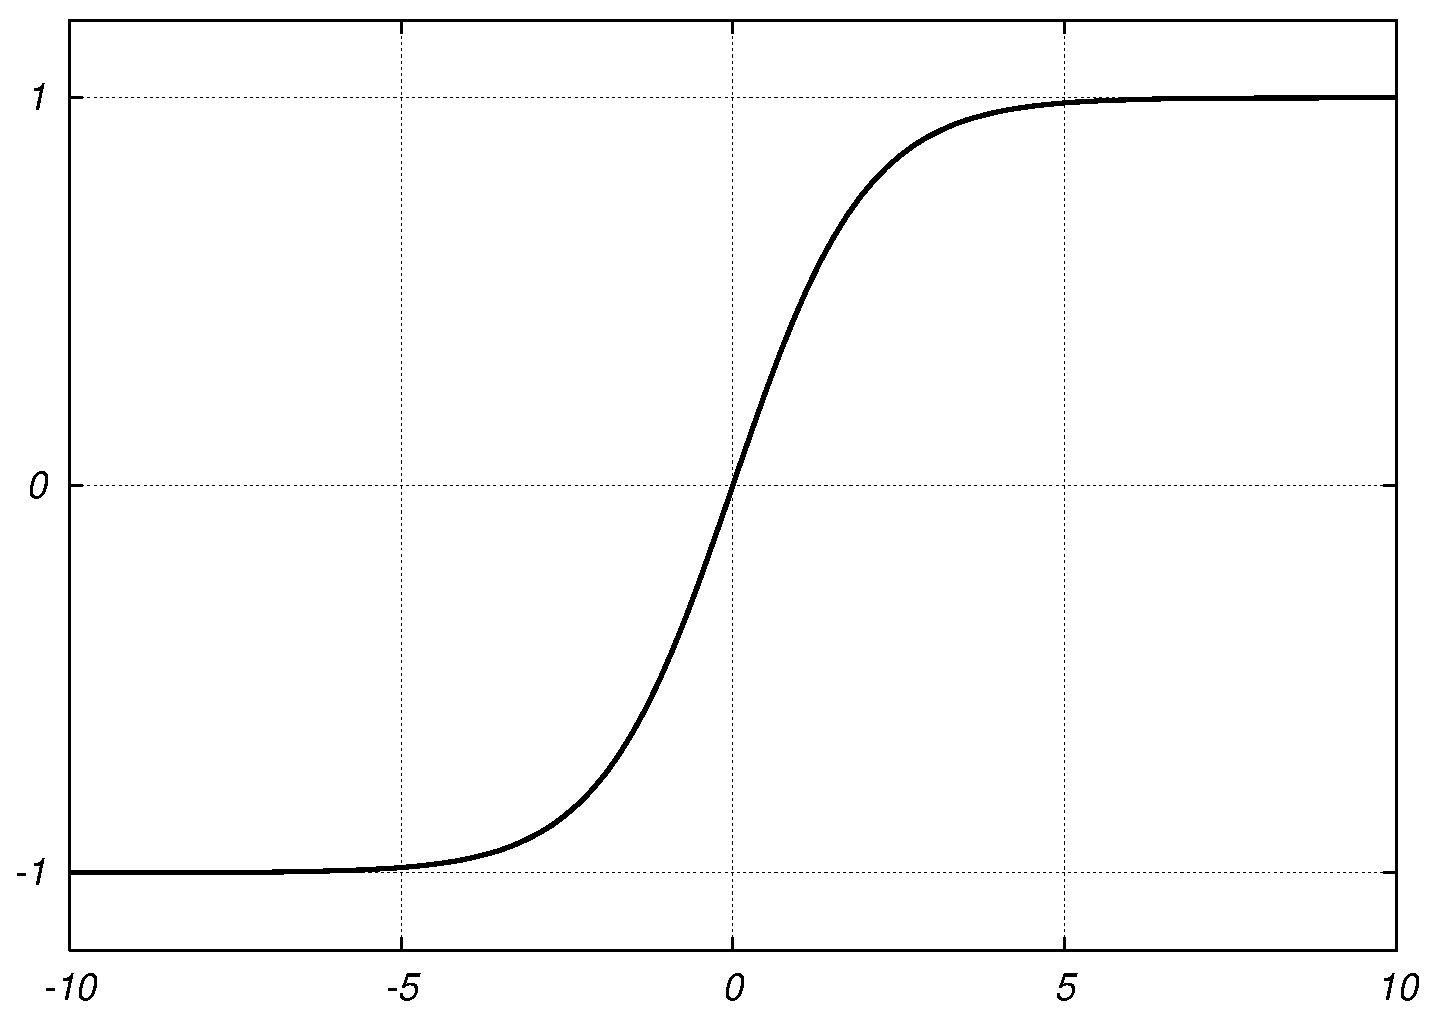
\includegraphics[width=0.45\textwidth,%
  totalheight=0.25\textheight]{tanh} &
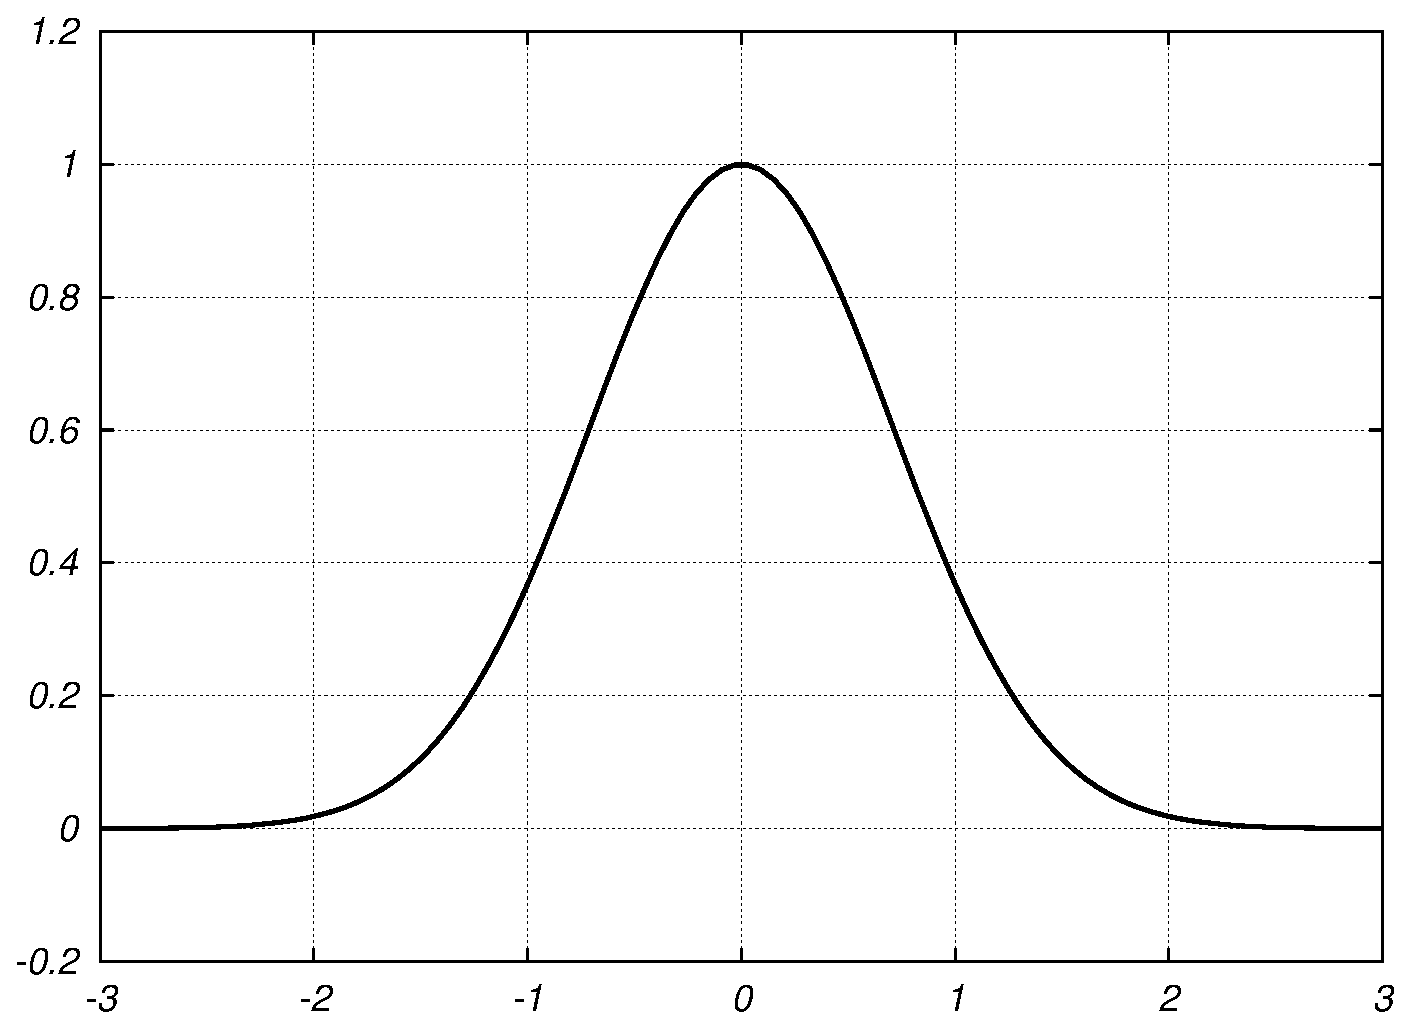
\includegraphics[width=0.45\textwidth,%
  totalheight=0.25\textheight]{rbf} \\
�) & �)\\
\end{tabular}
\caption{������� $\fa$ �������������� (�) � ���������-��������� (�) �����.}
\label{fig:act_func}
\end{figure}

���������� ������� ����������� ������������� ������������.  ������� �
����� ������ ���� ������������ � ���� ��������.  �� �����������
����������� ������� ���������� �������� � ���������������� �����
������, �� ����, ����� ������� ������� $i$-�� ���� �������� �� ������
�� �������� $(i+1)$-�� ����.  ����� ������������ ��������� ���� ���
������������ � �������� ������ ���������� �� \figref{fig:mlann}.

\begin{figure}[h]
\centering
% This does not make picture in PDF/LaTeX:
%\input{nn_arch.pic}
% So, let's do the next way:
% 1. xfig -specialtext -latexfonts -startlatexFont default nn_arch.fig
% 2. Update all text objects (with TeX special symbols) to Default font
% 3. Export to PS/LaTeX (changing default extension from .pstex to .eps)
% 4. Edit nn_arch.eps_t file and remove .eps extension from \includegraphics
% 5. Put next \input:
\input{nn_arch.eps_t}
\caption{������������ ��������� ���� ������� ���������������.}
\label{fig:mlann}
\end{figure}

��� ����������� �������� ����������� ������������ ��������� ����
������ ������������ ����������� $\NN_{n_0,n_1,\ldots,n_{m-1},n_m}$,
��� $n_0$ --- ����� ������ ������� (��������) ���� ����,
$n_1,\ldots,n_{m-1}$ --- ����� �������� � ���������������
������������� ������� �����, $n_m$ --- ����� �������� (� �������)
����������, ��������� ����.

%\subsection{����� ����� �������� � ����������� ����}

����������� ����� ���������� �������� � �� ������������� �� �����
�������� ������� ���������.  � ����������������, ���� ���� � �����
������������� ���������� --- ������� ������������� ��.  ��������
������������ ������ ������ �� ����� ��� ��������� ������� �������, ��
���� ���������� ���������� � ���������� ����� (��������, �������������
������ �� ������ �� � ���������-�������� ��������~\cite{koh80}).
����� ���������� �������� � ���� ������ ������������ �����������
�������������� �������.  � ����� ������, �� � ���������-��������
�������� ������� ���������� ������� �� ������ ���������� ��������, ��
� ��������� �������.  ��� ��������� �������� ���������������� ���
���������� � ������������ ����� �����, ����������� �������
������������ ��.

%\marginpar{����� �������?}
%�������� ������� � ���������������� ����������� ���� �������
%��������������� � ������������ $\NN_{n,k,m}$ � ������������� ��������
%���������~(\figref{fig:act_func}�).  ��� ���� ��������� ���������
%����������� ���������� �������� �������� ���� ��� ������� ������
%������������� $N$ ������� ��������� �������:
%\begin{equation}\label{eq:neuron-number}
%\displaystyle\frac{mN}{(n+m)(1+\log_2N)} \le k \le
%m(N/n+1)+\displaystyle\frac{m}{n+m}(N/n+2)
%\end{equation}

������������� ������ ������� ��������� ���� � ������������
$\NN_{1,n,1}$ ��� ����� ������������� � ������������ � ����� ����
������ � \cite{sontag93}.  ��� �� ����������, ��� ���������
������������� ��������� ����� ������� ������������� ��, �����������
�������� �����������, � ����� ������ �������� NP-������ ���������.

������, �������� ����������, ��� � ����������� ����������� ������� ���
������������� � ������ ��������� ������������ ����� ��������.
��������������� ������ ��� ������� ����������� ����������.  ������
������ ������������ ����� ���������� ����� ������������� �������� � �
������������ ������� ��������� �� ��������� ������ � ����������
�������.

��� ������������� �������� �� ����� ����� ��������� �������������
���������, ������������ �� ������������ ������.  � ���������,
��������, ��� ����- � �������������� ���� ������������� ����� �������
�������� ����������, ��� ����������� � ����������� ������ �������
�������������.  � ��� ������, ���� ��������� ���� �� ������ ����������
������, ������������� �������� �� ��� ����� ��������������� ����������
(���� ���������� ���������������, ��������� � ������������
��������~\cite{wasser92}).

�������� ����� �������, ������������� � ���������� ��� ��������
�������� ��� ���������� �� ������������ ���������� ��� �������
���������� ������~\cite{gibb96}.  ������ ������� ���������� ����
������� ��� ������� ����� ���������� ������ ����������.  ��������,
����������� � ���� ������� ��������� ������ � ������ ������������
��������� ���������������� ��������� ������.

%\subsection{������������ ����������� � ������������� ����������}

� ��������� ���� ������� ��������������� ����������� ������ ����������
������������ �� ������.  ��� �������� ������������ ������� ���������
����� ������������ ��������� �������:

\begin{itemize}

\item
������������ ������ �� ���� �� �������� � ���������������� �������
������� (\figref{fig:dynamic_nn}�);

\item
��������� �������� ����� � �������� ���� ��� �� ������������
������������ ����: ���� ������ � ��������~\cite{gibb96,golovko01};

\item
���������� �������� ����� � ��������� ����: ���� �������� � ��������
��������������� ������ �� �������
(\figref{fig:dynamic_nn}�)~\cite{wasser92,golovko01}.

\end{itemize}

\begin{figure}[h]
\centering
\begin{tabular}{cc}
\hbox{\input{dnn_arma.eps_t}} &
\hbox{\input{dnn_feedback.eps_t}} \\
�) & �)\\
\end{tabular}
\caption{������� �������� ������������ ������� ��������� ���� � �������
         ���������� �� ��������� ��� (�)
         � ���������� �������� ������ (�).}
\label{fig:dynamic_nn}
\end{figure}

% �������������� ����������� �� ������ ����

%\subsection{��������� �������� ��������� �����}\label{nn_learning_algorithms}

��������� ��������� ���� �� ������� ���������� ���������� ������
�������������� ����� ����������� ��� ����������� ��������� �������
$w_j$ --- ������� ������������� ��������.  � ������ ���������-��������
�������� ���������� ����� ������ $c_j$ --- ������ �������.  � ���
������, ���� ��������� �� ������� ��� ������� ������ �������������
��������� ����������� ������� $f(.)$, �������� ��������, �� �����
������� �������� ��������� � �������� ({\em supervised learning}):
\begin{equation}\label{eq:supervised_learning_task}
  \begin{array}{c}
    \mathbf{y}_k=f(\mathbf{x}_k)\\
    \sum\limits_k\big(\mathbf{y}_k-\NN(\mathbf{x}_k)\big)^2\rightarrow\min
  \end{array}
\end{equation}

������������ �������� �������� � �������� �������� ������
������������� ������� ``����������� ���''.  ���� �� ������� ������� ��
������ ����, �� ������� ��������� ��������� �������� �� ����������,
���� ������� ���������� ��������� ��� ������� ({\em unsupervised
  learning}).  �����, ��������, �������� ������� ������ ������������ �
������� ��������� ���� ��������~\cite{wasser92}.

��� ������� ����� ������� ����������� ������� �������, ������� ������
�������� �������, ��� �������, ������, ������� ����������
��������������� �������� ������ �������� � ��������.  ���� ���
�������� �� ����� ������ � �������� �����������, ������� ������� �
�������� ����� �������� �������� ������.  � ���������, ������
����������� ������ ����������� � �������������� (���������� ������).

������� ����������� ������� �������� �� �������� ��������
��������������� ������.  �� ������������� ������������ ������
����������� ������� �������, ��� ������� ��� ������ �����������
������������ ���������� � ������ ����������� ������� ������.
��������� ���������� ������, ��������� � ����������� ��������� ������
��������, ����������� � ��������� ������� ������� �������.  ����� ���
���� ��� ������������� ���������� ��� �������� �� (QuickProp,
Delta-Bar-Delta � �. �.), ��� � ������� ������ �������� � ������
����������� (������ ����������� ����������, ����������-��������� �
�. �.~\cite{himmelblau75}).  ������������� ����� ����������� �������
�������� �� � ��������� � ���� �������� ���������� �~\cite{gibb96}.

������ ������������ ����������� ������� �������� �������� �������
�������� ����������, �������� �������� ������� ������� �������.
������ ������������ ��������� ������ ����� �������� � ���������
������� ������ �����������.  � ����� ������ �������� ������
����������� �������� ����������� ������� �� ����� ���� ������.

�������� ������������ ������, � ������, ��������� � ��������� ��������
�������� � ������� ������ ������� ���������� ������.  ���� �� ���,
�������� {\it alopex}, ����������� �~\cite{boquete99}, ������� ��
���������� ������ � �������� ������� ������������� � ��������������
���������� ���������� ��� �� ���������� � ������ �����������.  �������
�������� ����� ����� ������, ��������� ��� �� �������� � ����������
���������-����������~\cite{wasser92}.  ������ ���������� ���� � ����
������ ������������ ``������������'' ����.  �� ���� ���������
����������� ��� ������������� �������������, ��� � ������� ����������
���� ������� ������������ ����������� ��������.  � ���������, �
������� ��������� ������ ���������� ������ ����������� ���������
�����������.  ����� ����, � �������� ���������� ������ ����� �� �����
���������� ������ ���������� �� �������� ��������.

������ ������� ������������� ���������� � ������ ������� ���������� �
����� ������ ������ ����������� ��������, ��� �������, ����������
��������.  � ������ �������, ����������� ������ ���������� � ���������
� ������������ �������� ����������� ������������ ���������� �
�������������� ������������ ���������� �������� � ���������������
������������� �����������.  ��� ����������� �������� ��������� ���
������ ����������� ������� �������� ��, ��� �������������� ��������� ��
������������� ������������� � �������� ��������������� ����������.

%%%%%%%%%%%%%%%%%%%%%%%%%%%%%%%%%%%%%%%%%%%%%
%\section{����������� ���������� ��������� ����� � �������� ����������}
\section{���� ��������� ����� � �������� ����������}

������ ���������� ����������, ��� �������� �� ������������ ��������
���������� ��������� ���� ����� ��������� � �������� ���������� �����
� ���������� ������ �����.  ������ ���� ����� ���� ���������, ���
����������� ������������ ���������� �� ����������� ��������� ���� �
�������� �� ��������.  � ����������� �� ������������� ����� ���������
���� ��������� � ����� �� ��������� �������:

\begin{enumerate}

\item
����������~\cite{sigom00,khomyu96,kav96,bouchard01,linwaihong01,gorfeld96,tukin01,pican95,golovko01,fabri98};

\item
������ ������� ����������~\cite{narmuk96,park96,levinar95,kulee96};

\item
������������ ������� ������� ����������~\cite{hayyeeder97};

\item
���������� ��������� � ����������� ������� ����:
��������~\cite{steck96,sigom00,chenmills97,vas-bak2009} �
�������-����������~\cite{sigom00,wailinlin00,linwaihong01};

\item
����������� ���������� ������� ����~\cite{sigom00,samtar96};

\item
�������������� ��� ��������������
�������~\cite{uhrig91,zhuchkov02,basubart94,golovko01}.

\end{enumerate}

� ���������� �� ����� ������������� ������ ������������� ����������� �
������������ �������, ��� ��� ��� �������� ��������������� � �������
�� ����� ���������� ����� ����������.  �������������� �������� ��
������������ ���������� ����������� � ����������� ��������� �����, �
����� ������������ ���������, � ����� ������� ���������� ������������
������ ������� ����������.

%\subsection{������������ ���������}
\section{������������ ���������}

%%%%%%%%%%%% �������� ��������� ����� ��������� �� ������

% ���������� �� ����������

������� ������������ �����������, ������������ ���������� �����
������������ ��� �� ����������, ��� � �� ����������.  � ���������,
������������ �������� ���������� �� ����������, � ������� ���������
���� ���������� ����� ������� ����������� ���� $\NN(e_k)$ (��������,
�~\cite{ronco98}).

% ���������� �� ����������

����������� ������������� ���������� $\NN(r_k)$, ��� $r_k$ ---
�������, ��������������� ���������� �� ����������, ����������� �������
������~\cite{khomyu96}.

% ����������� ���������� feedforward+feedback

��������������� ����� ��������� ������������� ���������� ������ �����
����������� ������ ���� $\NN(r_k,y_k)$, ��� $y_k$ --- ����� �������
����������~\cite{narpart92,trc95,samtar96}.  �������� �����������
��������� ����� � ���������� ������������� �������, ������������� ����
������� ������������ $\NN(e_k,y_k)$ � $\NN(e_k,r_k)$, ��� ���
$e_k=r_k-y_k$.  ������������ ��������� (��--�) � ������������ ������
$\NN(e_k,y_k)$ ������������ �~\cite{narmuk96}.

����� ���������������� ������������� ���������� ����������
�~\cite{sigom00}.  � ������~\cite{park96} �������� ����� ������������
��� ������������ ���������� ���������� ������������ ��������.  ���� ��
��������� ����� ($\NN^{FFC}$) �������� ����������� �� ����������, �
������ ($\NN^{FBC}$) ���������� ���������� �� �������� ����� �������
���������� � ���� ����� �������� �����.  ����������� ����������� ��
������ ����������� � ������������ � ����������:

$$
u_{k}=\NN^{FFC}(r_k)+\NN^{FBC}(r_k, y_k, u_{k-1})
$$

\noindent
��� $r_k$ --- �������, $y_k$ --- ����������� ����� ������� ����������,
$u_{k-1}$ --- ����������� �����������, �������������� � ����������
������ �������.

% ������ �����
� ��������� ������� ������������ ��--� � ������������ ���������
�������� �� ������� �������� �� �����.  ��������, �������� ����������
���� ���� --- ���������� ������������ ������� � ��������� ���� �������
���������������.  ��������, ����� ������� �� ���� �������������
���������� �������� ���������� ����������� ������� � ������� ��������:
$\NN(r_k,\dot{r}_k,\ddot{r}_k)$.  ���� ������� ������������� �
�������� ������ ����������� ������� ������:
$\NN(e_k,\dot{e}_k)$~\cite{wailinlin00,linwaihong01},
$\NN(e_k,\dot{e}_k,\ddot{e}_k,\ldots,{e}^{(n)}_k)$~\cite{eremin95}.  �
��������� ������ ���������� ����������� $n$ ������������ ��������,
������ �� ������� �������.

�������� �� ������ ���������� � ���������� ������������� ��������
��������� ������������� ���������� � ������ ����������, ��������
�������� ������ � ��������� ������ ��� ��� ���� ����� � �������������
���������� ������ ��� ������� ������.  �� � ����� �� �������������
����� ������ �� ������������� ����� ������, �������� �� ��������
���������� ��������� �����.  ��� �������, ����� ����� � ������������
������ ��--� �������������� �� �������� � ���������� ������������ ���
�� ���������� �����������.

% ��������
���������� ������������ � ���������� �������� ������� ���������
������������� ����������.  �� ���������� ������ ������� �����
���������� �~\cite{sigom00}.  �������, ��� � ����� ������ ������
�������� �� ������� �� ���� � ���������� ������ ��--�.

%\subsubsection{������ ��������� �������������}%
\label{direct_inv_nnc}

������ ��������� ��--� � �������� ���������� �� ���������� ��������
��~\figref{fig:direct_nnc}�.  ���� ����� ������������� ��� �������
���������� �� ����������� ������.  ��� ���������� ������������ �������
������������ �������� ����������� �� ���� ��--� ����������� �� �������
����������� �� ������ ������� ��������~\figref{fig:direct_nnc}�.  �
�������� ��������� ��������� ���� ��������� ������ �������� �������
����������.  �� ��������� �������� ��--� ���������� � ������
����������, �� �� �� ���� �������� �� ����������� ��������
$y_k,y_{k-1}$, � �������� $r_k,r_{k-1}$.  ����������� ��������,
��������� ���� ���������� ����� ����������� ����������� $u_k$, �����
����� ������ ���� ������ ���������.

\begin{figure}[h]
\centering
\begin{tabular}{c}
\hbox{\input{nnc_direct_inv_tr.eps_t}} \\
�) \\
\hbox{\input{nnc_direct_inv_ev.eps_t}} \\
�)\\
\end{tabular}
\caption{������ ��������� �������������: ����� �������� (�)
         � �������� ���������������� (�).}
\label{fig:direct_nnc}
\end{figure}

�������� ����������� ����������� ����� �������� ������������� � ���,
����� ������ ���������� ��� ���������.  ��� �� ������ ����� �����.
����� ����, ������ ���������� �������� ������� ������� ����������
�������� �������� ������� ���������� � ������� ��������
������������������ �������, ������������� ��� �������� ��--�.  �����
����� ��������� ������������� ������ � ����������� ����������� ������
� �������, ��� ������ �������� ��������� ���� ����� ����������
����������.  �������� ��������� �������� �������� � ������� ��������
��������.

%\subsubsection{������������������ ��������}

������ ����� �������� ��--�, ����������� ��~\figref{fig:special_nnc}
(��� ���������� ������������������ ��������), ������������ ����������
������� ������������� ��������� ���� � �������� �� ��������
����������������.  ����������� �������� �������� ��--� ����������
���������� �� ������ ���������� � ������������ ������ ���� �������.
��� ���������� ������ � ������ ������������� ���������� ����������
����� ���������� �������� �������� ������� ����������.  ��� �� ������
��������, ������� ����� �������������� ������ ��������, ������������
�����������, � ������� ���� �������� ����������� ����������� ���
���������� ������ ����������.

\begin{figure}[h]
\centering
\input{nnc_special_tr.eps_t}
\caption{����� ������������������� ��������.}
\label{fig:special_nnc}
\end{figure}

��������� ����������� ���������� ������� �������� ����������������
������ ��������� ���� � ������ ������ ��������.  ���������
������������ � ��������� ��--� ��������� ��������, �� ���� ���������
�������� $u_0$ ����� �������� � �������� ������� ���������� �
���������������� ������������.  �������� �� ��, ��� ������ �����������
� ���������� �� ��������������, ��������, ��� ������������������
�������� � ������ ���� �� ��������� �� ��������.

%\subsubsection{��������� ���������� �������������}

��� ��� ����������, ������ ����������� �������� �������� �������
���������� ������������ ������������ ���������.  ���� ���� ����������,
� ����� ������ ������ �������� � ������� ��������� ���� ���������� �
�.~\ref{identif_and_nnp}.  ������� �������� ��--� � ��������������
������������ ������ ��������~(\figref{fig:indirect_nnc}) � ������
������� ���������� ��-�������: ��������� ����������
�����������~\cite{narpart92}, �������� ���������������� �� �������
(������), ��������� � ���������������~\cite{sigom00}.  ���������������
�������� ����������� �� ����, ��� ������ ������������ ������ ������
���� ������������ ���������� � ���� �������, ����� ���� ��������������
����� ���� �� ����� �������� � ������������ ������ ����������.

\begin{figure}[h]
\centering
\input{nnc_indirect_inv_tr.eps_t}
\caption{����� ���������� ����������� ������������� �������������.}
\label{fig:indirect_nnc}
\end{figure}

� ������� ������ ����� ���������� ������������������� �������� ��
����������� ������� ������ ��������.  ������ ������ �������������
������������� ��������� ������ ��������� ���������� ����������
����������� ������ � ���������� ��������.  ������������ ������ �������
���������� (��--�) ��������� �� ����� ��������� ��������������� ������
������� ������� ���������� �����, ��� ��������� ��� ����������
������������ ���������� � ���������� ������������ ��������� �������
��--� � ��--� ������������.  ��������, ��� ���������� ����� ���������
����� ��������� ������������ ������� ���������� � ��������� ����������
������� � ������� �������.

�������, ��� ���������� �������� ������� ���������� �������� ���������
������� �������� �������, ������������ �� �������, �������������� �
�.~\ref{direct_inv_nnc}.  � ������� �� ������ �������� ���������
����������� ���������� ��������� ��������������� ������.

%  � ������� �� ������ �������� �����������
%������� ���������� �� �������� ������������, ��� ��� �� �����
%��������� ��������������� ������ ���������� ����� ��--� ������������
%���������� ������ ��������, ��������� � �����, ����������� �������
%��������� �������.

����� ��������������� ����� ������������� � ����� �� ������� ��������
��������� ����� � ��������� ������� --- �������� ���������������� ��
������� ({\it backpropagation through time --- BPTT}).  ������, ���
������������� ���������� �� ��� �������� ������ �������� ����������
���������� ����������� ���������� ������ � �������, ����� ��������,
��� BPTT, �������� �������� ��������� �����~\cite{narpart92}.

� ������~\cite{fabri98} ������������ ������������ ����� ������������
�������� ������������� ����������, ���������� �� ������������
���������� �������� ����������.  ��� ���� ���������������, ���
������������ ������ ������� � �������� ��������� �������������
������������� �����.  ����� ������������ ��� �������������
������������� ����������� �������, �������� �� ����������, � ����������
������� � ������ ����������.  ������������� ����������� ������ ��
��������� � ������� ������� �������� ���� ���������������� ���������
������� � ������ ������� ������� ������ ���.  ��������������� �������,
���������� ��� �� ������������ �����������, ��� � �� ���� �������� �
���������-�������� ��������.

%\subsection{������������ ������ ������� ����������}

%� ���������� ������ ��� ������� ������ ������� ������������� �������
%���������� ���������� �������� ����� ��� ������ �������� ��������
%����� ���� ����� �������.  ���� ``����--�����'', ����������� �� �����
%���������� �� �������� �������� ��������������� ���������� �����
%������������ � ���������� ��� ��������� ��������� ���� ��� �������
%������� ����������-���������.

%\subsection{������������� � ������������ ������ ������� ����������}%
\section{������������� � ������������ ������ ������� ����������}%
\label{identif_and_nnp}

��� ������� ������������� ����������, ������������ ��������� �����
����� ����������, ��������� ������ � ������������� ��������� ������
���������� �� ��������� �����.  �� ������ ���������� ��������, ���
������������ ��������� ����������� ����������� �� ������ ����� ����
���������� �������� �������� --- ������� ������� ����������� �������
��������� ������� ���������� �� ���������� ������������ �����������.
����� ���� �������� �������� ������� ������� ���������� �� ��������
��������� � ��������.

� ������������ �������� ������� ����� �������������� ������������ ��
������ ������� � ��� �������� ����� �������������� ��� ���������
��������� ���� ����������.  ������ ��� ����������� �������� ��������
���������� ������ ���������� �������� ��� �������� � ������� �������
�������������.

������������ ����� ������������� �������� ������ ����������
������������ �� ������������ ����������� ��������� ������� ��
���������� �������������� � �� ��������� �������, ����������� ���
��������� ���������� �������.  ������ ������ � ������ ���������
�������������, ��������� ���������� �� ���������� ������� ��������.

����� �� �������� ����������� � ������� ��� ���������� �� �����������
����������� ������� ������������� ����������� ���������� �����������
������ �������� �������� �������~\cite{bolonchin91}.  �� ���������
���������� ���������� ������� $A$ ����������� ���������� ��������
���������� ������� ����:
\begin{equation}\label{kachmaj}
\mathbf{x}_k=A^T \mathbf{u}_k
\end{equation} ��� $\mathbf{u}_k$ --- ����������� �����������, �
$\mathbf{x}_k$ --- ����������� ��������� ������� ����������.

������ ����� ������������� ������� �~\cite{boxjenk74}.  �� ������� ��
���� ������, �� ������ �� ������� ����������� ������� � ���� ������
�������, � �� ������ ���������� ��������� ������ � ����������� ��
�������������� �������������.  ������ �������� � ����� ���������
����������� ���������:
\begin{equation}\label{arima}
x_k=\delta^{-1}(B)\omega(B) u_{k-b} + n_k
\end{equation} ��� $B=1-\nabla$ --- �������� ������ �����, $n_k$ ---
��������� ������, ����������� ��������� ����, $\delta$ � $\omega$ ---
��������.

������������� ������ ����������� ������� � ��������� � ����������
������������ ������� ���������� � �� ���� ������� ����� �������� ���
������������� ���������� ��������, �������� � ��� ������, ���� ���
������������ �������� ����������.  � �� �� �����, ������������
��������� ��������� ����������� ���������� �������, ������� ���
���������� ������ ������������� ��� ��� ����� ����� �������� ������
�������� ����������.  �� ���� ������� ������������ ���� ������
���������� ������ ������� ��� ���������� ����������� �� �������������
��� ������ �������� ����������� ������������ ������� ����������
������������� �������������, ������ ��� �������� ��� ������ �������
������� ����� ����������.

%%%%%%%%%

���������� ������������ �������������, ��� ������������ ������������
������� � ��� �������� ���������� ����� ������ �������� ��� �������
������������ �����������.  ��� �������� ���������� ������ ����������,
����������� ������� SISO ({\it single input, single output} --- ����
���� � ���� �����).  � ���������� ������� � �������� ������������
��������� ������ ���������� ����� ����������� ��������� ��������
���������� ���������:
\begin{equation}\label{eq:siso}
\left\{\begin{array}{rcl}
  \mathbf{x}_{k+1} & = & f(\mathbf{x}_k, u_k) \\
  y_k & = & g(\mathbf{x}_k)
\end{array}\right.
\end{equation} ��� $y_k$ � $u_k$ --- �������, � $\mathbf{x}_k$ --- ������
��������� ������� � ���������� ������ ������� $k$.

��������� ���� ������� ���������������, ����������� �������
$\hat{y}_{k+1} = \NN^o(u_k)$, ������������� �� ����� ������ ������
�������� ��������� ������������� ������� \eqref{eq:siso}, ��� ���
��������� �� �������� �������: � ����� ������ ����� ��������� ����
������� ��������������� ��������� ������������ � �����������
������� � �� ������� �� ��������� ��������� � ���������� �������
�������, � ����� �� ������� ������.

��� ���������� ���������� ������������ ������ ������� ��������
��������� ����������� � ������� ����������.  � ���������� ��
������������� ���������� �������� ��������� �������� ������� ����
��������.  �������� ��������� �� ��� ������������ �������������
�������� ������ ������ ��������� ���� ��� ���������� ��������� �����
�������� �������.  ������ ������� � ���������� ������� �������� ������
� ������� ��������� ������� ���������������.  ������ �������
������������ ���������������� ���������� ���������� ������� ����������
� ����� ``���������'' ��������� � ��������� ������������� ������� �
���������� ������� �������.  ��������� ��������� �������� ������,
������������ ��� ����������.  ���������� �� ���������.

%\subsubsection{���������� �������� �����}

���� �� ��������� ��������� ������ � ���������� ���������� ���������
���� ��������� �~\cite{boquete99}.  ����������� ��������� ������������
������ ������������ ����� ����������� ������� ���������-�������� ����
� FIR �������� � ��������� �������� �����.  ���������������� ������� �
������������ ������ �����������
����������~\eqref{eq:rbf_neuron_output}, ������ ���������-��������
������� $R(.)$ ����������� �� ����� ������� �������, ����������
��������� �������� �����:

$$
R_j\bigl(\mathbf{x}(k)\bigr)=
   \exp\Bigl[-\frac{1}{\sigma^2}\sum\limits_{i=1}^M
             (x_i(k)+\tilde{x}_{ji}(k)-c_{ji})^2\Bigr]
$$

$$
\tilde{x}_{ji}(k)=\sum\limits_{s=1}^S a_{jis}R_j\bigl(\mathbf{x}(k-s)\bigr)
$$

��������� ����� ��������� ���� ���������� � ������� ���������������
������������ ������ � ����� ����� ��������� ������� �������������
��������� ���� $w_i$ � FIR ������� $a_{jis}$.  �
������~\cite{boquete99} �� ���������� ������������������ �������
������ ������� �������� ����� $S$.

������ ������� ������������ ������, ������������ �~\cite{benne00}
����� ����������� ���� ������~\cite{golovko01}.  ��������� ���� �����
������� �����������
$\hat{y}_{k+1}=\NN^o(u_{k-1-n_L},\ldots,u_{k-n_b-n_L})$, ��� $n_b$ ---
�������� �������� �������� ���������, $n_L$ --- �������� ��������
�������� ������������.  ����������� ���� ������� �� $n_a$ ��������
$\hat{y}_{k},\ldots,\hat{y}_{k-n_a+1}$.  ��������� �����������
������������ ������ $n_a$, $n_b$, $n_L$ ������������ ��������� ��
��������� ��������� ������ �� �������.

%\subsubsection{������� �������� �����}

������������ ������ ������� � ������ ������� ������� ����������
�������������� ������, �� ������� �������� ����� ������,
���������� � ���������� ������ �������~\cite{sigom00}:
$$ \hat{y}_{k+1}=\NN^o(u_k, \hat{y}_k) $$

����������� ������ �������� ����� $\hat{y}_k$ ����� ����� ������
���������.  ����� ������ ���������� ��~\figref{fig:nnp-feedback}.

\begin{figure}[h]
  \centering
  \input{nnp_feedback.eps_t}
  \caption{������ � ������� �������� ������.}
  \label{fig:nnp-feedback}
\end{figure}

��� �������� ��������� ����� � �������� ��������� ������� �����
������������ ����� ��������� ��������������� �
�������~\cite{gibb96,sigom00}.

������������� � ��������������� ������ ������ ������ ����� ��
������������, ��� ��� �������� ��--� ��������� ������ �������
��������� ��� $(u_k, y_k)$, ���������� ��� ���������� �������� �
��������� �������.  ��� ������ ��� �������� � ��� ����������������
������ �� ������������.  ��� ��������, ��� ����� � ������ ���������
(��������) ������ ����� �� ����������.  ������������ ������ ������� �
������ ������ �������� ��������� ����������.  ��� ��������� {\it
��������� }�������.  ������� �������� ������������� ���������� ��
������������ ������ ��������� �������� ��� ������� ����������.

������ � ���������� ���������� � ���������� BPTT.  �������� ��������
�������� ����� ������� � �������������� ��������� ����������, �������
����� ������ ��� ���������� ������� ��������� ���� �� ����������
����������� ������� ��� ����������� ��������� � ��������
�����������~\cite{levinar95}.  ����� ����, ����������, ��� ��������� �
�������� ��������� ������� �������� �������� ����������� � ���������
������������������, �� �� ����� ��������� ������� � ���� �������������
���������� ���������� � ����������� � �������� ����� � ��������
��������� ��������������� ������~\cite{linetal}.  ��� �������� �������
�������� ����������� ��������� ({\em vanishing gradient}).

������������� � ������ ������������ �������� ������� ����������
�������� ����������� ��������� ��������� � ���� �������:
\begin{itemize}\label{simple-feedback-defects}
  \item ������������ ������ ������������ � �������� �������
  ����������;
  \item ��� ����������� ������� ������� ��� �� ��������� �
  ����������� �������� ����������� ��������������� ������.
\end{itemize}

%\subsubsection{���������� ������� ���������}

�������� ����� ������ ��--� ����� ��������, ���� ������������ ���
������������� ������������� �������� ������� ��������� ������� ���
���������, ������� ��������������� ����������� � ���������� �������
�������.  � ���� ������ ������� ������ ������� ���������� ������ ���
�������� ������ �� ������ �������� ���������� �� ������� ����������:
\begin{equation}\label{eq:past-states}
  \hat{y}_{k+1}=\NN^o(u_k, u_{k-1},\ldots,u_{k-D_u}, y_k,
                           y_{k-1},\ldots, y_{k-D_y})
\end{equation}

������ ������ ����������� �� ������ �������, ��������
�~\cite{kulee96,levinar95}.  ����� ����� �� ��������� ������� �
����������� ������� ��������� ����������
��~\figref{fig:nnp-past-states}.

\begin{figure}[h]
  \centering
  \input{nnp_paststates.eps_t}
  \caption{������ ������ � ����������� ������� ���������
  $\hat{y}_{k+1}=\NN^o(u_k, y_k, y_{k-1})$.}
  \label{fig:nnp-past-states}
\end{figure}

�������� ���� ������ �������������� ��� ������� ���������� ��
��������� �������� �������, ���������� ��������� ���� $u_k$ � $y_k$.
��������� ���� $\NN^o$ ��������� ������ ������� ���������
������� ����������� ������ � ������� �������������� ��������.
��������� � ������ ����� �������� ����� �����������, ��������
������������� ������ �� ������� �������� ����������� ��������� �����,
��������, ������������ ������ ��������� ���������������.

����� ������ �������� ����������� ��������� ����� �������������� �
������� ���������� ��� ������������ ������ ������� � ��� ���������
���������������.  ����� ������ �� �������� ����������.  ��� ���������
�� ���������� �� ��������, � �� ��������������� �� ���������� �����
��������� �������.  ����� �������, ��� ������ {\it ������������
}������ ������� ����������.

������ ���������� ������� ��������� ����� �������������� ��� ��������
������� ����������, ������ ���������� �������������� ������ ����������
������������ ����������� ��������� ������� ���������� ��� ���
�������������� �, ������, ��� �������� ���������������.  �����
�������, �������� ������������� ���������� ������ �������������� �
������� ���������� � ������ �������� ����������������.

%\subsubsection{��������� ������}

������� ��������, ��� �������� ����������� ����� ������� � ������
������� ���������� �������, ����� �������� ������������
��~\figref{fig:nnp-hybrid}~\cite{park96}.  �� ����, � ������
����������� �������:
\begin{equation}\label{eq:nnp-hybrid}
  \hat{y}_{k+1}=\NN^o(u_k, u_{k-1},\ldots,u_{k-D_u}, \hat{y}_k,
                              \hat{y}_{k-1},\ldots, \hat{y}_{k-D_y})
\end{equation}

\begin{figure}[h]
  \centering
  \input{nnp_hybrid.eps_t}
  \caption{������ ��������� ������
  $\hat{y}_{k+1}=\NN^o(u_k, \hat{y}_k, \hat{y}_{k-1})$.}
  \label{fig:nnp-hybrid}
\end{figure}

��� �������� ��������� ���������� ������������ ����������� ��������
��������� ��������������� �� �������, ����������� ��������.

� ������ ������ ��������� ������� ����������� ������ � ��������
��������� �������.  � ���������, ����������� �� �������� �������
������������ ����� ������������� ����������� ������ ������ ����������
������ ����������, � �������� ����� � ����������� ����������
����������� ������� ��--� --- ������.

�� ��������� � ������� ���������� ������� ��������� ������� ����������,
��������� ������, ��-������, �������� ����������, ��-������, ���������
���������� ����� ������ � ����� �������� �������� �������.

������ ���������� ��������� ����� ��� ���� ������������ ������������
���������� ������� � �������� ��������� ������� (� ��� ����� �
���������).  ��� ��������� �������� �������� ���������, �� �������
���������� �������� �������� ��������� ��� �������� ������.

%\subsubsection{������������� ������}

� �������~\cite{narmuk96,ronco98} ������������ ������������
��������� ������� ������������, ������� � ������ ������ ������� �� ��
���, ������� ���� ��������� ����������� ������������ ������ �������
����������.  � ������~\cite{ronco98} ��� ������ ������ ������������
���������-�������� ��������� ����.  ��� ��������� ����� ������������
��������, ����� ������ ����������� � ����� ����������.

����������� ������������� ������� �� ������������ ��������� �����-����
������� �� �� �����������.  � ���������, ��� ����� ���� ���
������������, ��� � ������������ ������.

%\subsubsection{���������� ���������� ��������}

������������ ������������ ������� ��������� $E=\frac{1}{2}(\hat{y}_k -
y_k)^2$, ������������ ��� ��������� ������������ ������ ������� ���
������� ����������, ������� ���������� ������� �����������������
������� ��� ��������� ���������� ������.  ��� ����������� ����������
������ ������ �������������� � ������������ ��������� ������� �������
�������.  � ������~\cite{wangbao00} ��� ����������� ���������� SISO
������ ������� ������������ ������������ ���������������� �������
���������, ���������� ��������������� ������ ������ ��������:

$$
E=\frac{1}{2}\Bigl\{\bigl(\hat{y}_k - y_k\bigr)^2 +
  \lambda\bigl(\frac{\partial\hat{y}_k}{\partial u_{k-1}} -
  J^B_k\bigr)^2\Bigr\}
$$

\noindent ��� $J^B_k$ --- �������������� ������� �������, �������������
������������ $-J^B\le J^B_k\le J^B$, � $\lambda$ --- �������
�����������, �������, ��� ������������ � ������, ������ ���� ������
�������.  ���������� ��������� ������ ������������� �������� ��������
��--� � ��--�, ������������� ������������ �������� �������������
��������� ��������� �����.  ������������� ������� ��������������
����������� ������������ �������������, ���������� �� ����������
�������� � ����������� �������.

%%%%%%%%%

\section{������ ������� ���������� ��������� �����}

%\subsection{���������� ������������� ����������� ��������� �����}

��������� ���� ����� ������������ � �������� ���������� �����������
��� ��������������� � ������������ ������ �����, ������ ��������� ���
�����������~\cite{steck96,sigom00,chenmills97,vas-bak2009}.

����� ������ ���������� ������������ ������������ ����������� �
������������� ��������:

\begin{itemize}

\item
������������� ����������� � ������� ��--� ���������� ��������,
������������ ��� ������������ �������������;

\item
��������� ������� ���������� � ���������� ��������� ������� �������
��� ����� ����� ���������� ��--�;

\item
������������ ������� � ��--� ����������� �������� ������� � ���
�����������;

\item
���������� � ������� ��������� ���������� ������� ������������
��������� ������, ����� ����������� ��� ����� ������������
�������������.

\end{itemize}

��������, ��� ���������� �������� � ������������ ����������� ��������
�������� ���������� ����������� ����� ��������.  �������� ������� �
���� ������� �������� ��������� ������� ������������ ����������� ��
��������� � �������������.  � ��������� ������� (��������,
\cite{chenmills97}) ���������� ��������� ����������� ��������
������������ �����������.  � ������~\cite{warwick96} ��������� ����
����������� � ������� �������������� ������������ �������� ������
����������, ��� �������������� ������� �� ����� ���������� �������.
% ������������� �������� ��� ������������������ ���������
������~\cite{khomyu96} �������� ���������� ��������� �����������
���������� �����, ������ �������������� ���������� ����� ������������
��������, �� ����������� ������� ������������ ������� �� ����������� �
����� ���������� �������.  ������ � ���, �� � ����� �� ���������
������ ����� �� ���������� ���������������� ��������������
������������, ������������ ����������� �������� ������������ ��������
� ������������ ����������� � �������.  ������������ ������
������������ �� �������� ��������, ��� ��� �������� ������� ���
��������� �������, ��� � �������������� ��������� �������������� �
���������.

� ���������� ����� ����������� ������� ���������� �������
�������-���������� ����������� � ���������
�����~\cite{sigom00,linwaihong01}.  ����������� ������ ��������������
�� ������ ���������-�������� �����.  ������� ��������� � ���� �����
����� �����, ����� ������������ ��� ����������� ��������
��������������.  ����� ��������� ������� ���������-�������� �������
�������� ����� ����� ������������� � ����� ������ �������-�����������
�������.  ������ �������� ����� ����������� ����������� ������������,
� ��������� ������������ ��������� ���������� �����������
����������~\cite{wailinlin00}.  � ���� ������ �������-����������
������������ ��������� ������� ����������� � ��� �����������, ���
��������� ������������� ������������ ������� ������������ �
����������� ����������� ������, ���������� � ��������������� �������
����������.

%\subsection{����������� ������������ ����������}

������� ����� ��������� ������ ���������� ��������.  � ����������
������ ���������� ��������� ������������� ������� � ����� �� ��������
��������� ����������� ������ �������� � ������� �����������
����������.  � �������������� �������� � ������ ���������� �������
������ ���������� ������� �������� � ������� ������� �������.  ��� ��
�����, ���� ��������, � ������� ���������� ������������ ����������
������������.

������������ ������ � ����������� ���������� ���������� ����������
�~\cite{hayyeeder97}.  ������ ����������� �������� ������ � ������
������� � ���������� ������ �� ������ ��������� ���� �
���������-��������� ���������.  � ������ ���������� ����������
��������� ���������� ������������� ������� � ����������� ����������
�������.  ������������ ����� ������ ������������� ������������� �
������ ������������ ��������, ������������ ����� � ���������� ��
������������ ����������� � ��������� �������.


%\subsection{��������� ���� � �������� ����������� ����������}

� ��������� ������� ������������ ������������ ���������� ��������
��������� ����� �� ��������, � �������������, ��� ��������� ����������
������� ����.  ��������, �~\cite{samtar96} ��������������� ���
�������� ������� ���������� ��� ���������� � �������������� ���������
����.  ������ ������ ������������ ����� ����� ���������� �����������
���������� � ���������� ������������ ������� �������, ������������ ���
��������� ��� ����������.  ���� ������� ������� ����������� � ���,
����� �������� ������������ ������ �� ��� ��������� ���������
���������� �������������� ����������: $K_P$, $K_I$, $K_D$
(��.~\figref{fig:nn-tunes-pid}).

\begin{figure}[h]
  \centering
  \input{nn_tunes_pid.eps_t}
  \caption{��������� ��� ���������� � ������� ��������� ����.}
  \label{fig:nn-tunes-pid}
\end{figure}

� \cite{sigom00} ���������� ������� ����� ��������� ��� ����������,
������ � �������� ������ �� ������������ ������������ ������ $r_k$,
$u_{k-1}$, $y_k$.  ��������� ����������� ��������� ������������
������������ ������� ��������� $E=\frac{1}{2}(r_k-y_k)^2$.

������������ ������ ������������ ������������ ������������ ������� �
������ ������ ��������� ������� ����������.  ������������� ���
���������� �������� ������ ������������, ������ ��� ����������
�������� �� ������ ������� ������������ ��������� ����� �����
�����������.

\section{������������� ������������ � �������� �����������}

����������� ������������ ������� ���������� � ����������� �����
�������� �� �������� �������� ������ ���������������
�������������~\cite{warwick96}.  ��� �������� ��� ������� ��������,
��������������� � �������� �����������, ��� � �����������, �
����������� �����, ��� (�� ���� � ������, ��������, ����������
84\%~\cite{sigom00}).  ������� ��������, ��� ��� ��������� ��������
�������� �������� ��� ������������� � ����� ������������ �� ��� �����.

�������� ������~\cite{vukobrat1991} �� ������� ���������� �����
������������� ������ ���������� �������������� ������������� ������
��������� ��� ����������� � ������� ��������� ���� ������������ �
������ �����.  �������� �������������� ������������ ������� ��� ������
������� ������ ���������� ��������� ������ �������������� �������, �
��� �����, � �������������� ��������� �����.  � �� �� �����, ���������
���� �������� ����������� ���������� �������� � ��������� �� � ������
���������� ����������� ������ �������� ���� �������.

� ������~\cite{khomyu96} ���������� ���������� �������������
�������-�����������, {���������\-��\-��}, �� � ��������� �����������
���������� ({\em general predictive cont\-rol\-ler}).  ���������
�������������� �� ������� ���������� ������������ � ��������.  ������
������������ ��� �������� ������� ���������� (����������� � ������
������� ����������, ����������� �������������, ��������������
��������� ������������ ����������), ��� � ��������� ���������� �
��������� ��������� (����������� �������, ������� ������, ���������
������� �������� ������� ���������� � ������ ��� ����������).
�������� ����������� �������� ���������� � ��������� ����������
����������� �����������.  ������, ���������� � �������������� �������,
����� ��������������� �������� (``�����'', ``������'', ``������'',
``����� ����''), ��� ��������� �������� ������� ����� ������
������������� ��� �������������� ������ ���.  ������ �����������
���������� � ���������� ��������� ��������� ����� � ���������
��������� � ������� ������������.  ������ ���������� �� ����
���������� ������� ������ ���������������� ��������������� �����������
�� ��������� ���������, � �� ����� ��� ���� �������� ��������� �������
��������� �� ����������� �������� �������� ������ ��� �������������� �
������� ��� ������ �����.  � ������ ������ ��� ��
�������~\cite{sigom00} ����� �� ���������� ����� ��������� �������� �
����������� �������������, �������������� ���� ���� ��������� ��������
���������� �� ��������� � �������� �������.

� ������~\cite{boquete99} ���������� ������� ������ �������� � �������
�������� � ������� ��� ������������� � ������������ ���--��
�������������.  ����������, ��� ���������� �� ��������� ���������
����������������� � ��������� ������ �������, ��� ��������������
������� ��������� ����.  ������ ������ �������� ������ ��������
���������� � ������ �� ����������.

������ ������ ������������� ��������� � ������������� ����������
����������� �� ������ ���������� ������������ ����������
�~\cite{wailinlin00}.  ������ ��������, ��� ������ ����������
���������� �������������, ������ � �������� ������������ ����� �����
����������, ����������� ��������� �����������, ����������� ����������
�������� ���������� � �� ����������� � �������.  ���� ����� ����������
������������ �~\cite{vukobrat1991}.  ���������� ���������
������������--��\-���\-��\-��\-��\-��\-���� ���������, ������������
�������� �~\cite{wailinlin00}, ��������� ���������� � �������� �������
���������� � ������������ ������, �������� ��������� �����������������
��� ����������� �������� � 3 ���� �� ��������� � �� ���������.
������ �� ���������� ���������� � ����� ����������� ����������
����������� �������� �� ��������� �������, � ������������ ��������� �
������ ������������� �� �������� ����������� ��������������������
������.

����� � ������� �� ������������� ������������� ��������� �
������������� ������������ ����� ���������������� ��������, ��� ����
�������������� ���� ��������� �������� ������������� �� �����������
��������.  ����������� ������������, ��������������� ������������
�������� ����������� ����� ������������� � ��������� ��������
�����������.  ��������, ����� ������� ������ ����, ������ ��
���������� � ���������� ��������������� � ��������� ������ �� ����������
�� � �������� ����������.

������� ����������������� � ������������� ���������� ����� ���������
����� � �������� �������� ��������������� � �������~\cite{warwick96} �
\cite{toudeft}.  � ������ ����������� ����������, ��� ����������
�������� ���������� ��� ������������� ���������� �������� ����������
����������� ���������.  ����� ����� �������� ������������ ����������,
������� ���������� ������� ��������� �������� �, ��������� ����������
���������� � ��������� ��������� ����, �������� � ������ �
������������� �������������� �������� ������ � ������� ���������
�����.  ��� ���������, ���������� ����� ���������� �������� �
���������� ���������� � �������� �������� � ���������� ������ �������
�������� ����������.  ���������� ������ �� ����� ��� ��������, �����
����� �� ����� � ������ ������������ ���������� ��, ��� ������� ����
�������������� ������� ��������� ������������� ��� �������� ��������
�������� � ���������� ���
(��������,~\cite{khomyu96,wailinlin00,elfil-pta99}).

�� ������ ������~\cite{toudeft} ��������� ��--� �������������� ��
����� ���������� ����������� ���������� �������� ������������ ��������
� ������ �������������.  ��� ������� ��--� ������� ������� ���������
���������, � ������ ������������ ������������ ������������ ��������
������� �� ����������� ����������.  ����������� ������ ������ � ���,
��� ��������� ���� ��--� � ��--� ������������ �� ������ ������� �
�������� �������.  �������� ����� ���������� �������� �� ����
��������, ������� �������������, ��� ������ �������� ���������� ������
������ ������������� ������������� ������� ``������������'' ������� �
������ �������� ����������.

��� ������������ �������, ��������, �������� ���������������������,
��� ��� � ����� ������� ���������� ��������� ���� ������������ ��
��������.  ��� ���������� ���������� --- �������������� �
������������� --- �� ���� ������������� � ���, ��� �� ����������
��������� ���� � ������ ���������� �������� ��������.

�������������� ���������, ��� ��������������� ��������� �������������
� ������������� ��������� ���������� �������� ������ ��� ����������
���������� ����� ������� �����, ������ ��������� ���� �������
������������� � �� �������� ���������������� � �������� �����������
���������� ��������.  � ����������� ����������� ������� ������
������������� ���������� �������������� �� �������� �����������
�������������������� ������ ����������.  �������� ������ ������� ���
���������� �� ����� �� ��������, ������ ���������� ��������� �� ������
������������� ������ �������� ���������: ������������, ��������������.
������� � ����������� ������������ ������� ��������� $K_I$, $K_I$,
$K_D$ �������������� � ������� ������ �� ��������� �������, ����
����������� �� ������� ������� �� �����������
�������~\cite{kurop73,netush68}.  ���������� � ���� ������
��������� �������� ����� ������������, ����������� ����� �����������
��������, ����������� ����������������� � �. �.  ��������, ��� ���
���������, �������������� ����� ����������� ��������, �� ������
��������� ���������� � ������������, �������������� ��������������������
������ ����������.

%\subsection{������ ������������ ��������������� ����������}

��������� ������ ������� � ������� �������� ��� ������ ���������� ���
������� ����������������� ������.  ����������� � ��������������������
�������� ��� �������� ������ ��������� � ����� ������� ��������������
������.  �������� ��������� ������--����� �������� ���������
����������� �������� ������, ����������� � ��������������������
������~\cite{solod60,skliar65,ostrem73,tsipkin58}.  ���������
��������� ������� ����� ������� (�, ��������������, ����������)
�������� ������� �������������������� ������, �� ��������� ��������
���������� ���������� ��� ��������� � ������������.  ����� �������,
��� ��������� ������� ��������� � ���������� �������� ������������
����������, ��� ��� ������������� ������������ ������������ ����������
�� �������� ����������� � ���������� ������.

� ��������� ����� ����������� ����������� ��������� ����� �����������
� ����� � ��������� ������������ � �������� ���������������
����������, ��� ��� �� �������� ����� ����� �����������:

\begin{enumerate}

\item
�� ��� ������� ������� ���������� ��������� ���������;

\item
�� ����� ������������ ������ ������������;

\item
�������� ������� ����������������� � �������� ������������� ������� �
��������;

\item
����������� ������ � ��������� � ���������� ������� ����������.

\end{enumerate}

��� �� �����, ����������� ������ ������ ��� ���������� ������������
�������������, ��� ��� ��������� �������� ������������ �������� ������
������������ ������ ����� ������������ ������������� � �����������
�������� ��������� ��� ��������� ������� ����������.  �����
����������� ����� ����� ������ � ������� �� �������� ������ �������,
������ �������� ���������� ����������~\cite{bramziff82,ostrem73}.
���������� ����� ������������� ����� ������������� ������� ������
����������� ��������� ���������� ��� ��������� ������� ������� ����,
��� ��� �������� � �����������.  ����� ����, � ���� ��������
�������������� ������������ ���������� ������� ������ ������� ��������
�������.  ������ ������� �����������, ������� ����������� ������ �
������������ ����������� (������������
����������������~\cite{brisynho72}, �������
���������~\cite{leondes70}), ������ ����������� ��� ������� �����
���������� � ������ �����������, ��������, ��� ������� ������������ ��
�������������� ����������.  ��� ��� ����������, ����������,
��������������� �� ����� �������� ����������� ���������� �
�������������, ���������������� �� �������� �����������
�������������������� ������ ����������.

�������� ����� �������� ���������� �������������������� ������ � ��������
������� ��������� ��� �������� ��������� �����, ����� ������ ���������
� ���������� ������ ������������� ������������� --- ��� ���������
������� ������������ ����������.  ������ ������ �� � ������ ������ ���
�������������.  � ����������, ��� ��� ����������, ����� ����������
���������� ������������� ��������� �����������, ������ �������
���������� �� ��������� ��������� � � ������� �������������.

����� �����, � ������� ����� ���������� �� ����������� ���������
�������������� ������������� ����������, �������
��������~\cite{fabri98} �~\cite{liao99}.  ������ �� ��� ���������
�������� ������� ����������, �������������� � ���������������� �
�������� ����������������, ��������, � ������ ������� �����������
�������, ����� �� ��������� ��� �� ����������������� ����� �������
�����.  ��� ������ � �������� �� ����������������� ����������� ������,
����������� ������������� � ������� ������� ��� ��������� ������
��������� �� ������ ������� ������ ����������.  ������ ���������� ���
���� ����� ���� ����������, �� �������� �� ����������.

�� ������ ������~\cite{liao99} ��������������� �������� �������
������������ $N$ �������� ������������� ����������, ������ ������
�������� �� ����������� ���������� �������.  ������ ���������������,
��� ������ ���������� �������� � ��������������.  � ��������
���������� ������ ����� ��������� ������������ ��������, ���������
������� �������������, ����������� � ������������ � ������� ������� ��
���������������.

���������, ������� ��������, ��� �������� ������������� ��������
����������� � ������������ �������������� � ���������� �� ���������.
����� ����, �������������� ���������� �������� ��������� �������������
� ������������ ������������ �����������, ��������� ��� �������� �����
����� �������� ������� ���������� ��������� ����� � ��������
���������� � ������������ ������������ �������� �� ������������� ���
�������� � ������ ������������� ��������.

%%%%%%%%%%%%%%%% ���������� �����
\section{����������� ��������� ��� �������� �������\-����� ������ ����������}

��� ��� ����������, � ���������� ������������ �������������
��������������� ������ ��������� ��������� ���� �������
��������������� �������� ��������� ��������� ������, ������� �
���������� �����������, � ����� ������������� ������������� �������.
��� ����������� ��������������� �� ������ �������� ������������ �����
� ������� ����� �� ������������ �������.  ������ ��� ���� �����������
��������� �������, ��� ���������� ������� �������� � ��� �������������
��������� ��������� ���� � ������ ������� ���������� ����������
������.  ��� ���������� �� ����� ������������� �� ������� � �������� �
������� ��������.  ����������, ������������ ����������� ��, ������
�������� � ��� �����������, � ����� ��������� ������ ���� ����������
�������, ������������ � ������ ������� ������������� ��.

������ ��� ������������ ����� �� ����� ������������� ��������� �����
������������ ��� ��� ���� ������������� (Statistica, MatLab, Octave �
��.)  ��� ������������������ ������������ (Stuttgart Neural Network
Simulator, Neural Lab, Trajan � ��.) ����������� �����.  ���
����������� ������� �����, �������� � ������� �� (�������������
�������, ������������� ������, �������������, ������������ � �.�.),
������������ ������������� ������� ������ ����������.  � ���
���������:
\begin{itemize}
\item ������� ����������� ��������� � ������ � ��������.
\item ������� ���������� ���������.
\item ������� ���������� ��������.
\item �������� ��������� ����.
\item ������ �������� ������ ��������� ��������� ����.
\end{itemize}

������ ���������� ��������� ����� � ������� ���������� �������
������������� ������� ������ �������, ������������� � �������
������������� �������������:
\begin{itemize}
\item ������� ���� � ���������� ���������� � ������� ����������.
\item ������� ������� �������� - ������� � ������.
\item ���� ������ �� ��������� ����� ������� ���������� ���
  ������������ � �������� ��������� ����.
\item ������������� ���.
\item ��������� � ������ �������� ������ ��� � ����������
  ������������, � ��� �����, � �������������.
\end{itemize}

� ������������� ������� (������ MatLab) ���������� �������������
������� ������� ���������� ���������� ���������������� ���
��������������, ��� � ������������� � ����������� �������.  � �� ��
�����, ������������ ��������� �������� �� ������������
���������������, ��� ��� ������ ���� �������� �� ����������������
����� ����������������.  ������� �������������� � ������ �����
��������������� ���������� ���������� �����, ��� ��� ������������� �
�������� ��������� ����� ������������ �� ������� ��������� �����
(������� $10^4 ... 10^6$ ��������).

��� ����� ������� ��������, ��������������� � ������� �����, ��������
���������������� ���������, ���� ����� ����������� � ��������� �
��������� ��� online-������������� (��������,
\cite{inv-pend-osc-base,nn-online-training-tool,neuroph-online-demo}).
����� ��������� ������ ������������� �����-�� ���������� ��������
���������� �� ���������� �������, ��������, ���������� ��������
���������, ������� ����� � online-����������� ��������� �����������
�������� ��������� ����������, ������� ��� ������ �� ����� ����������.
��� ���������� ������������� ������������ ���������� ������������
������ �������.  ������ ������� ����������� ������ ��������� ���������
������� � ����������� �����������.  ��� ��������� ������������ ������
��� ������������ ������������ ������� �, � �����, ���������� �������
������ ��������.  � ������������ online-�������� ��������� ��, ��� ��
�� ���� ������������� �� ���������, ��� �� ���������� ������������
�������� ������������ (�� ����������� web-��������, ������������� ���
������� �� web-�������� ���������) � �������� ����� � ������, ��� ����
������ � ��������.

� �� �� �����, � �������� ��������, ����� ���������� ��� ���������
����� ��������� ����������, ���� ���� ����������:
\begin{itemize}
\item ����� ������������� �� ����� ���������� ������, ������ �����
  ���� � �������������� �����������;
\item ��������������� ��������������, ���������� �� ������������
  ``�������'' �������� ��������� � ��������������� ������ ���������;
\item ������ ����������� ����������� ��������� � ����� �����������
  ����������.
\end{itemize}

����� �������, ���������������� online-��������� ����� ����
������������ � ������� �������� ����� ����������� --- ��� �����������
������ ���������� ����������� ���������� � ���������� �������.  ���
������������ �������, ��������������� ���������� ������� ���������,
��� ���������� ����������.

�������������� ���������� ����������� ������������� ����� ��������,
����������� ������ ������ ������������� ���������� � ������������
������������ ������� � �������������.  �� ���� ������ ������ �����
������� ���� ������������ ������� ��� ��������� ����������
��������������, ��������� ������������ ������ ������ � ����������
��������� ����� � �������� ��������������� ���������� � ���������.
���������� ������������ ���� �������� �������� �������� ��������
������, ���������� ���������� �� �������, ������������ ������ �������
������� �����.  ��� ������������ �������� �������� ��������
����������� �������� ��� �� ������� � ��� ����������������� ��������,
�������� ������ ��������� ������������� ������������� ��� � ���������
����������� ������������� � ��� ��������� �����.

%%%%%%%%%%%%%%%%%%%%%%%%%%%%%%%%%%%%%%%%%%%%%%%%%
\section{������}

\begin{enumerate}

\item
���� �� �������� ���� ���������� ��������� ����� � �����������
�������� ���������� --- ��� ������������ ���.  � ���������� �������
�������� ������������ ���� ���������� ������������� ��������� �����
��� ���������� ���������, � ����� � ������ �������������� ���������
��������������� � ������������ ������.  ���� ������������ ����������
������������ ����������� ��� ����������� ���������� � ������������
������ ����������� �������� ����� ������� �� ���������� ����������.
���������������� ��������� ����� � ��� ������������ ������������
����������� ��������� � ���������, � ����� ������ ���������� ��������,
�������� ������������ ��� ������������.

%�������� ����� ���������� ��������� ����� � ����������� ��������
%���������� --- ��� ������������ ��������� ������������ ���.  ����
%������������ ���������� ������������ ����������� ��� ���������� �
%������������ ������ ����������� �������� �� ���������� ����������.
%���������������� ��������� ����� � ��� ������������ ������������
%����������� ��������� � ���������, � ����� ������ ���������� ��������,
%�������� ������������ ��� ������������.

%������� �������
%����� � ���, ��� ������� ������ �������� � ��� �� ������� ������������
%������������ �������.  � ���� ������ �������� ��������� �������������,
%� ��� ����� �������������, ������ ������� ���������� �������.
%��������� ���� ���������� ������� � ������� ������� �����
%������������� ����������, ����������� ����������� ������������ �������
%�������: ��� ������������� � ������������ �������.

\item
������������� ������� ������������� ��������� ����� ���� ������������
������, � ���������, �������� �������� ������ ������ �����������
����������� ��� ������� ���������� ������.  �� ���������� �����
������������ �������� ������������ ����������� ��������� �������.  ���
��� ������� ����� ��� �������� ������������� ��������, ����������� ���
��������� �������� ���������� ��.  ������������ ������� ���������� ��
� �������� ���������� � ���������� �������� �����: ������ ����������
����������� ������� �� ������������� ������� ������ ��� ��� ����
����������� ��, ���� � ������ ��������� �������.  � ����� � ����,
������ ���������� �������� ������ �������� ������� ��������� ����� �
����� �������������� �� ���������� � �������� ����������.

%����������� ����� ��������������� ������������� ������ � ��.  ���
%������� ����� ��� �������������� ��������.

\item
��� ���� ������������ �������� ���������� ��������� ����� � ��������
��������������� ���������� �������� ������ �������������� ������������
���������� ���������� ����������� ����������.  ���������� �������
������� ��������� ����������� ��������� ���������� ����������
����������� ��� �������� ������� �������� ����������, � ��� �����
���������� � ��������������.

%�������� ������������� ������ - ��������� ��--� �� ��--� - ������� ��
%���������� �����, ������������ �������� �����, � ����� �������� ������
%���������� �������� ������� ������������� ������������ ��.

\item
������� �������������� ����� �������� ������ ������������ ���
����������� �������������.  ����������� ������ � �������� ������������
�� � �������� �������� � �� ������������ ������������ ����������� ��
��������� � ���������.  ������ ������ �� ������ �� ����������, �� ����
�� �������� � ����������, ������� ������������ ����������.
�������������� �������������� �������������� ����������� �����������
���������� ��������� ����� � �������� ��������.

%������������� �������������� ������� ������������� � �������������
%��������� ���������� �� ������ ������������ �������.

\item
���������� ��������� ����������� ������ ����� �������� ������ ���
����������� ��������� �������, ������� ������������� ��������
��������� ������������� � ������������ ������������ �����������.  ���
������� ������������� ������������ ���������� ���������� ������������
��������� ��������� ����������� ��������� �����, ������������� �
��������� � ��������� �������� � ����������� ���������� �����������
���������.  ������� ������������ � ������������ �������� ����� �������
������ � ������������� ����������� �� ���������� � ������, ������
��������� ������� � ������ ��������������� ������, ��������� ��������
��� �������������� ������������ ������ ����������.

\item
����������� �������� �������� ����������� ������������� ���������� �
����������� ����������, ������������ ��� ������������� ������
���������� � �������� ��������� �����.  ���� ����������� ��
������������� �� ���� �� ������ ���������������� �������.
������������� ���������� ������������ ������ ��� ������� �
����������������� �����, ������������ ������� ���������� ���������
����� � ���.

\end{enumerate}


% Глава 2
\chapter{Метод синтеза нейросетевого оптимального регулятора}
Просто описание методики синтеза регулятора без ответов на вопросы
``почему так?''  Строго конструктивно.
%\input{part_noc_synthesis.tex}

% Глава 3
\chapter{Выбор архитектуры нейронных сетей и параметров их обучения}
\centerline{Краткий план главы}
\begin{enumerate}
\item Выбор архитектуры нейронных сетей для регулятора и модели
  объекта управления.  Рассматриваются наряду с принятыми решениями
  альтернативные варианты.  Если есть материал, то иллюстрируется
  почему так, а не иначе.
\item Подбор длины обучающей выборки.
\end{enumerate}
%\input{part_nn_arch_and_params.tex}

% Глава 4
\chapter{Сравнительный анализ нейросетевого оптимального, ПИД и винеровского регуляторов}
Рассмотреть в том числе зависимость качества управление регуляторов от
частоты.  Фактически, материал второй лабораторной работы.
%\input{part_compare_controllers.tex}

% Глава 5
\chapter{Нейросетевое управление в нестационарных условиях}
По материалам двух последних статей --- в Вестнике МЭИ и в Ильменау.
%\input{part_non_steady_conditions.tex}

% Глава 6
\chapter{Нейросетевое управление мобильным роботом}
Как пример замены традиционного регулятора на нейросетевой для
управления реальным роботом.
%\input{part_mobile_robot.tex}

% Глава 7
\chapter{Программный пакет для моделирования и обучения методам нейросетевого управления}
%\centerline{Краткий план главы}
%\begin{enumerate}
%\item Цель работы: обучение и исследования
%\item Основные решаемые задачи
%\item Интеграция в учебный процесс и дидактические аспекты
%\item Описание лабораторных работ
%\item Описание программного комплекса
%  \begin{enumerate}
%  \item Структура комплекса и выбор инструментария
%  \item Основные интерактивные элементы
%  \item Вспомогательные интерактивные элементы
%  \item Сервисные и вычислительные программы
%  \item Объектная библиотека
%    \begin{itemize}
%    \item Абстракции данных и вспомогательный сервис.
%    \item Ввод-вывод, параметры.
%    \item Функциональные блоки от {\tt NaUnit} (+ .tf, .cof, .nn)
%    \item Нейросетевые элементы, методы обучения
%    \item Базовые структуры для построения сетей Петри
%    \item Объекты для моделирования дискретных динамических систем
%    \item Формализм для графического представления динамических моделей
%    \item Пример: дообучение нейросетевого регулятора в контуре
%    \item Пример: моделирование САУ и обнаружение разладки
%    \end{itemize}
%  \end{enumerate}
%\end{enumerate}

% -*-coding: cp1251;-*-
%%%%%%%%%%%%%%%%%%%%%%%%%%%%%%%%%%%%%%%%%%%%%%%%%%%%%%%%%%%%%%%%%%%%%%%%%%%%%%
% ����������� �������� ��� �������� ������� ������������� ���������� �
% ������� ��������

% ����:
% 1. ���������
%  1.1. �������� ������������ ������� � �������� ��
%  1.2. ������ ����� �����?
%  1.3. ������ ������������ �����
%  1.4. ������������� �������
% 2. �������� ������
%  2.1. �������� ������� (���������, �������������)
%  2.2. ����������� ������
%  2.3. ����� ����������� ���������
%  2.4. �������� ��������� ���������� � ��������
% 3. �������� ������������ �����
%  3.1. ������ ������������� ����������
%  3.2. ��������� ��-�, ����������� ������������ � ��� ����������
%  3.3. ������������ ���������� �������������� ��������

%\section{���� ������}

���������� ��������� ����� � �������� ���������� �������� ����������
����� ������������ ���������� ��������.  ������������ � ���� �������
���� ������� �������, ������ ���������������� ������� ����
������������ �����������.  � ���������, ��� ����������� �� ���, ���
����������� ������������� ����������� ������, ����������� �������
������������ ������ ��������������� ���������� �� ���������
�����������������.  ��� ���������� ��� ����� � web-��������.

� ������������ ���� ��� ����������� ���, ��� ������������� ����� ��
��������� ����� �� ��������� ������ �� ���� ����������� ����� �������
������ ���������� �����.  �� ��� ��� ���������� ��������� ����� --- ��
������ ������������� �������.  � ����� �������� ��������� ������� ����
�� ��������� ����� ����������� ������ �������� ������������ �������,
����������� ��������� ����������� � ������������ ���������������
�������� � �������� ����������� ����.

�������������� ���������� ����������� ������������� ����������� �����
��� ��������� � ������������� ������������ � ������������ ������
���������� � �������� ������.  �� ��� �� ������� ��� � ������ ��������
�������� � ����� ��������� ����� � ����� ������ ���������������
���������� �� ���������� �������������� �����, ��� � � ����������
�������� ��� �������������� ��������� ������ ����������.

�� ���� ������ ������������ ������ ����� ����������� ���� ������������
�����, ��������������� ����������� ��������� ����� � ������������
�������� � ������������� ����������� ��������� �� �������������
��������� ����� � �������� ����������.

%%%%%%%%%%%%%%%%%%%%%%%%%%%%%%%%%%%%
\section{�������� ������������ ������}
% -*-coding: utf-8;-*-
%\section{Описание программного пакета}

\subsection{Основные решаемые задачи}\label{main_tasks}

В соответствии со своим назначением программный пакет должен решать
задачи моделирования САУ, моделирования и обучения нейронных сетей.
Типовой сеанс работы с пакетом подразумевает интерактивное
взаимодействие пользователя с программами.  Поскольку пакет
разрабатывается для применения в учебном процессе, весьма желательно,
чтобы он был:
\begin{itemize}
\item простым в изучении и использовании;
\item адаптированным к специфике учебного процесса;
\item быстродействующим на не самых современных компьютерах;
\item открытым к модификации;
\item основанным на общедоступных и открытых технологиях.
\end{itemize}

При моделировании систем автоматического управления необходимо
предусмотреть возможность гибкой настройки контура и условий его
работы.  В частности, должны настраиваться:
\begin{itemize}
\item уставка (стохастическая, детерминированная);
\item помеха (стохастическая, детерминированная);
\item регулятор (линейный, нейросетевой);
\item объект управления (линейный, нелинейный, нестационарный).
\end{itemize}

%TODO: аргументировать, почему эти свойства важны.  м.б., в первой главе

В то же время, учитывая учебную направленность пакета, представляется
достаточным ограничиться одноконтурными системами управления когда
объект является одноканальным по входу и выходу.  Это существенно
упрощает интерактивную часть пакета и практику его использования.

Для моделирования и обучения нейронных сетей должны иметься следующие
возможности:
\begin{itemize}
\item создание нейронной сети с произвольной архитектурой в классе
  многослойных персептронов;
\item обучение нейронной сети на заданной выборке с контролем процесса
  по тестовой выборке;
\item предсказание поведения объекта управления с помощью нейронной
  сети в контуре в процессе моделирования;
\item обучение нейронной сети регулятора в контуре управления в
  процессе его моделирования.
\end{itemize}

Специфика применения нейронных сетей в системах автоматического
управления заключается в преимущественном использовании сетей класса
``многослойный персептрон'' с обучением методом обратного
распространения или более эффективными его вариантами.  По этой
причине нецелесообразно реализовывать поддержку сетей существенно иных
парадигм (Кохонена, Хопфилда и пр.).  Иногда применяемые в САУ
нейронные сети, основанные на радиально-базисных функциях (RBF),
доказанно являются эквивалентными многослойному персептрону, поэтому
их реализация тоже является избыточной и ради простоты программного
комплекса от неё целесообразно отказаться.

%\subsection{Структура пакета и выбор инструментария}
\subsection{Структура пакета и инструментальные средства}

Анализ требований к пакету обнаруживает, что некоторые из них трудно
совместить, пользуясь какой-то одной инструментальной технологией
разработки программ.  В частности, эффективное выполнение
вычислительных алгоритмов требует компиляции программ перед
выполнением.  Только с помощью компиляции можно обеспечить приемлемое
быстродействие на не всегда современных компьютерах, используемых в
учебном процессе.  В то же время, открытость к модификации
подразумевает возможность изменения программы прямо перед выполнением,
что важно для быстрой разработки, а также при углубленном изучении
пакета программ и проведении исследований с его помощью.

Кроме того, не все технологии разработки программного обеспечения
доступны на всех распространенных операционных системах: Microsoft
Windows, Linux, Mac OS X.  Некоторые из подходящих технологий
реализованы только в проприетарных программных продуктах,
использование которых требует покупки дорогостоящей лицензии.

В \tablref{tabl:sdk_tech} приводятся данные о сравнении нескольких
различных современных технологий разработки программного обеспечения
по перечисленным трем критериям.  Под технологиями в данном случае
понимается совокупность языка программирования, среды разработки и
выполнения и необходимые средства для реализации пользовательского
интерфейса и интерактивной графики.

\begin{table}[ht]
\centering
\caption{Сравнение технологий разработки программ.}
\label{tabl:sdk_tech}
\begin{tabular}{|l|c|c|c|}
\hline
\bf Технология & \bf Быстродействие & \bf Открытость к & \bf Общедоступность \\
             &                & \bf модификации  & \bf и открытость \\
\hline
             &                &  плохо       &              \\
\tt C++      &   отлично      & (требуется   & отлично      \\
             &                & компиляция)  &              \\
\hline
             &   средне       &  плохо       &              \\
\tt Java     & (интерпретация & (требуется   & отлично      \\
             & байт-кода)     & компиляция)  &              \\
\hline
             &   средне       &  плохо       & плохо        \\
\tt C$\#$    & (нужно много   & (требуется   & (в основном, \\
             & ресурсов)      & компиляция)  & для MS Windows) \\
\hline
            &   плохо        &              & средне       \\
\tt Python  & (интерпретация & отлично      & (нет унифициро- \\
            & байт-кода)     &              & ванной графики) \\
\hline
           &   плохо        &              &              \\
\tt Tcl/Tk & (интерпретация & отлично      & отлично      \\
           & байт-кода)     &              &              \\
\hline
           &   средне       &              & плохо        \\
\tt Matlab & (интерпретация & отлично      & (платный и   \\
           & байт-кода)     &              & очень дорогой) \\
\hline
\end{tabular}
\end{table}

Отсутствие идеальной технологии для разработки пакета моделирования и
нейросетевого управления вынуждает искать компромиссное решение.
Можно функционально разделить пакет на интерактивную и вычислительную
части и реализовать каждую с помощью оптимальной технологии.
Вычислительная часть требует эффективной реализации с точки зрения
быстродействия, поэтому целесообразно реализовать её на языке {\tt
  C++}.  Компиляторы этого языка программирования доступны для всех
значимых платформ, а сам язык, пожалуй, является в настоящее время
наиболее популярным среди универсальных процедурных языков
программирования.

Интерактивную графику и управление вычислительными алгоритмами важно
сделать максимально гибкими и открытыми для модификации.  Хорошим
выбором будет использование интерпретируемого языка с встроенными
возможностями для реализации пользовательского интерфейса, прикладной
графики и средствами интеграции программного обеспечения.  Одним из
подходящих инструментов является {\tt Tcl/Tk}, доступный бесплатно и в
исходных текстах для всех распространенных операционных систем.

Функциональная декомпозиция разрабатываемого пакета по используемым
технологиям разработки программ находит отражение в структуре
взаимодействия отдельных частей программного комплекса, которая
приводится на \figref{fig:prog_interaction_struct}.  Реализация
вычислительных функций в отдельных узкоспециализированных программах,
написанных на языке {\tt C++}, позволит пользователю гибко управлять
их взаимодействием и во многих нестандартных случаях снизит
необходимость в модификации текстов на {\tt C++}.

\begin{figure}
\centerline{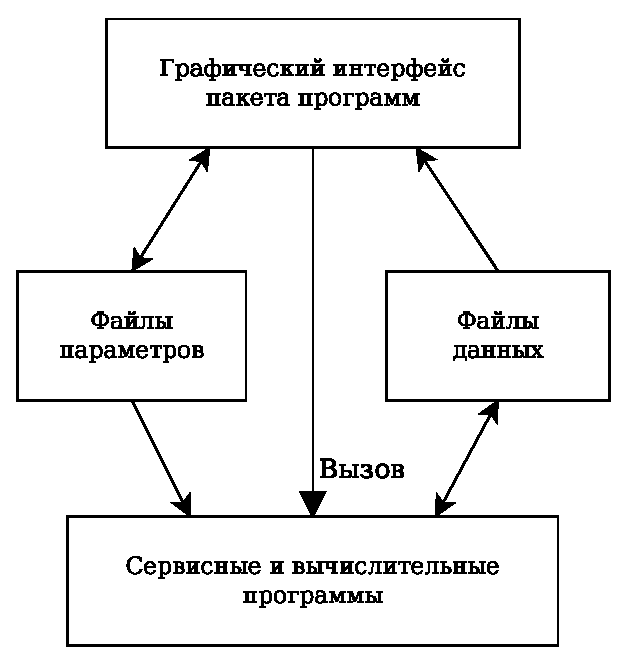
\includegraphics{princ_struct}}
\caption{Схема взаимодействия частей программного пакета}
\label{fig:prog_interaction_struct}
\end{figure}

\subsection{Основные интерактивные элементы}

Интерактивная часть пакета разрабатывается с использованием парадигмы
событийно-управляемого программирования.  Действия пользователя
порождают события, которые, в свою очередь, приводят к вызову
процедур, ассоциированных с ними.  Структура событийно-управляемой
программы имеет следующие особенности:
\begin{itemize}
\item Основной структурирующей единицей программы является окно.
\item Перед появлением окна на экране выполняется программный код ---
  процедура инициализации окна, --- формирующий внешний вид и основные
  интерактивные возможности взаимодействия с этим окном.
\item Внешний вид окна и его поведение может зависеть от параметров
  процедуры инициализации.
\item Процедуры-обработчики событий устанавливаются при создании окна
  или в процессе его жизни.
\item Внешний вид окна и его поведение в течение жизни может зависеть
  от действий, выполняемых в тех или иных обработчиках сигналов.
\end{itemize}

В соответствии с поставленными задачами целесообразно распределить
функции программы между окнами пользовательского интерфейса со
следующим назначением:
\begin{enumerate}
\item моделирование системы автоматического управления включая случай
  нестационарного поведения объекта;
\item создание/просмотр/редактирование цепочки линейных и нелинейных
  звеньев;
\item создание/просмотр/редактирование нейронной сети;
\item обучение нейронной сети модели объекта управления с
  использованием указанных выборок вне контура;
\item обучение нейронной сети регулятора с использованием указанных
  выборок вне контура;
\item обучение нейронной сети регулятора в контуре управления в
  процессе его моделирования;
\item просмотр заданных выборок (дискретных временных рядов) в виде
  графиков по времени;
\item просмотр заданной выборки в виде гистограммы для оценки
  одномерного распределения;
\item просмотр двух заданных синхронных выборок в виде множества точек
  на двумерной плоскости для оценки двумерного распределения.
\end{enumerate}

\subsection{Сервисные и вычислительные программы}
% TODO: перечислить наименование и назначение ряда программ

В соответствии с разработанной схемой взаимодействия компонентов
пакета моделирования (\figref{fig:prog_interaction_struct}) основные
блоки, выполняющие численные расчеты и обработку данных, не связанную
непосредственно с визуализацией графики, реализуются на языке
программирования {\tt C++} набором неинтерактивных программ.  Эти
программы взаимодействуют друг с другом и с пользовательским
интерфейсом не непосредственно, а через файлы параметров и данных.

Управление работой программ поизводится путем задания всех необходимых
параметров перед их запуском.  В различных программах в зависимости от
сложности их параметризации реализованы следующие способы передачи
параметров:
\begin{itemize}
\item в качестве аргументов командной строки;
\item через переменные рабочего окружения;
\item через файл с параметрами.
\end{itemize}

Конфигурационные файлы с параметрами различных программ имеют общий
синтаксис, описанный в \tablref{tabl:par_syntax}.

\begin{table}[ht]
\centering
\caption{Описание формата файла параметров.}
\label{tabl:par_syntax}
\begin{tabular}{|c|l|p{10cm}|}
\hline
Правило & Синтаксис & Семантика \\
\hline
1 & \tt \#                 & Однострочный комментарий \\
2 & \tt \em Имя = Значение & Параметр с заданным именем и значением до конца строки \\
\hline
\end{tabular}
\end{table}

Перечень вычислительных и сервисных программ с классификацией по
областям назначения приведен в \tablref{tabl:prog_list}.

\begin{table}%[ht]
\centering
\caption{Список вычислительных и сервисных неинтерактивных программ пакета.}
\label{tabl:prog_list}
\begin{tabular}{|c|l|p{13cm}|}
\hline
$N^0$ & Название & Назначение \\
\hline
\hline
\multicolumn{3}{|c|}{Основные программы моделирования и специализированного обучения нейросетей} \\
\hline
1 & \tt dcsloop & Моделирование контура управления. \\
2 & \tt dplantid & Обучение нейросетевой модели объекта управления вне контура  \\
3 & \tt dnnplant & Проверка функционирования нейросетевой модели объекта \\
4 & \tt dcontrp & Предварительное обучение нейросетевого регулятора подобно заменяемому вне контура управления \\
5 & \tt dcontrf & Дообучение нейросетевого регулятора в контуре управления с помощью нейросетевой модели объекта \\
\hline
\multicolumn{3}{|c|}{Неспециализированная работа с нейронными сетями} \\
\hline
6 & \tt MakeNN & Подготовка файла нейронной сети заданной архитектуры \\
7 & \tt ResetNN & Инициализация весовых коэффициентов нейронной сети случайными значениями \\
8 & \tt TrainNN & Обучение нейронной сети общего вида на заданных примерах \\
9 & \tt EvalNN & Проверка работы настроенной нейронной сети общего вида \\
\hline
\multicolumn{3}{|c|}{Генерация временных рядов} \\
\hline
10 & \tt dmeander & Генерация временного ряда вида ``меандр'' \\
11 & \tt drand & Генерация случайного временного ряда с заданными параметрами \\
12 & \tt drandmea & Генерация случайного временного ряда вида ``меандр'' с заданными параметрами \\
13 & \tt dsin & Генерация моногармонического временного ряда с заданными параметрами \\
\hline
\multicolumn{3}{|c|}{Операции с временными рядами} \\
\hline
14 & \tt dmult & Умножение значений временного ряда на указанное число \\
15 & \tt dsub & Вычитание значений временных рядов \\
16 & \tt dsum & Сложение значений временных рядов \\
\hline
\multicolumn{3}{|c|}{Обработка и изучение временных рядов} \\
\hline
% & \tt d2ts & Нумерация значений временного ряда \\
17 & \tt dconst & Проверка гипотезы о постоянном среднем значении временного ряда \\
18 & \tt dcorr & Расчет функции корреляции указанной длины для заданных временных рядов \\
% & \tt djacob & Расчет дискретной оценки якобиана по временным рядам управляющего сигнала и состояния одномерного объекта \\
19 & \tt dmean & Расчет среднего значения временного ряда \\
20 & \tt dmse & Расчет среднеквадратичной ошибки временного ряда \\
% & \tt dsmooth & Сглаживание временного ряда на скользящей базе  \\
% & \tt dstat & Расчет статистических параметров временного ряда нарастающим итогом \\
% & \tt dstatsb & Расчет статистических параметров временного ряда в скользящей базе \\
21 & \tt dstddev & Расчет среднеквадратичного отклонения временного ряда \\
22 & \tt dtf & Применение заданной линейной передаточной или комбинированной функции к указанному временному ряду  \\
23 & \tt Distr1D & Построение одномерного распределения временного ряда \\
24 & \tt Distr2D & Построение двумерного распределения временного ряда \\
% & \tt FileCvt & Преобразование формата файла временного ряда \\
25 & \tt StatAn & Расчет статистических параметров временного ряда \\
\hline
\multicolumn{3}{|c|}{Алгоритм кумулятивных сумм} \\
\hline
26 & \tt acstest & Проверка параметров АКС вне контура управления \\
\hline
\end{tabular}
\end{table}


\subsection{Объектная библиотека}

Объектно-ориентированная библиотека {\tt NeuArch} разработана на языке
программирования {\tt C++} и предназначена для реализации следующих
основных задач:
\begin{enumerate}
\item Работа с цепочками линейных и нелинейных звеньев: создание,
  выполнение, хранение в файлах.
\item Работа с нейросетями архитектуры ``многослойный персептрон'':
  создание, обучение, выполнение, хранение в файлах.
\item Моделирование динамических систем в дискретном времени.
\end{enumerate}

Кроме того, библиотека реализует ряд необходимых вспомогательных
функций: ввод/вывод временных рядов, чтение и запись файлов
параметров, абстрактные структуры данных и прочий сервис.

Библиотека является переносимой (функционирует на ОС MS Windows и
Linux) и универсальной, то есть, не содержит буквальной реализации
высокоуровневых функций, возложенных на программный пакет.

%fil% \subsubsection{Моделирование линейных звеньев}
\paragraph{Моделирование линейных звеньев}

Для моделирования на компьютере системы управления в целом необходимо
иметь компьютерные модели составных элементов.  Для описания линейного
элемента удобно воспользоваться z-преобразованием передаточной
функции.  Это представление является общепринятым в классе линейных
систем в дискретном времени.

В программном пакете передаточная функция $P^*(z)$ линейного элемента
описывается произвольной комбинацией следующих базовых конструкций:

\begin{equation}\label{eq:polyfrac}
P^*(z)=\frac{a_nz^n+a_{n-1}z^{n-1}+...+a_0}{b_mz^m+b_{m-1}z^{m-1}+...+b_0}
\end{equation}
\begin{equation}\label{eq:sum}
P^*(z)=\sum\limits_{i=1}^NP^*_i(z)
\end{equation}
\begin{equation}\label{eq:product}
P^*(z)=\prod\limits_{j=1}^MP^*_j(z)
\end{equation}

Несмотря на то, что действующую линейную передаточную функцию всегда
можно привести к полиномиальному виду \ref{eq:polyfrac}, удобно иметь
возможность произвольного описания.  Можно подобрать такую структуру
представления линейного элемента, чтобы коэффициенты имели легко
интерпретируемый смысл.  Например, ПИД регулятор удобно задавать в
виде суммы произведений полиномиальных дробей:

\begin{equation}\label{eq:pid}
C_{PID}^*(z)=K_P+K_I\frac{z}{z-1}+K_D\frac{z^2-2z+1}{z^2-z}
\end{equation}

В этом случае коэффициенты $a_0$ вырожденных полиномиальных дробей
$\frac{a_0}{1}$ приобретают общеизвестный смысл $K_P$, $K_I$ и $K_D$.

Пример представления конкретного ПИД регулятора

\begin{equation}\label{eq:pid_example}
C_{PID}^*(z)=-0.3+1.47\frac{z}{z-1}+0.02\frac{z^2-2z+1}{z^2-z}
\end{equation}

\noindent в формате, воспринимаемом пакетом моделирования, приводится ниже:

\begin{verbatim}
;NeuCon transfer 1.0
; Speed form of a discrete PID controller
[TransferFunction]
sum 3		 ; Kp + Ki*(z/z-1) + Kd*(z2-2z+1/z(z-1))
polyfrac 0	 ; <=== Proportional term
 -0.3 /  1	 ; Kp
product 2	 ; <=== Integral term
polyfrac 0
 1.47 /  1	 ; Ki
polyfrac 0
 1 0 /  1 -1
product 2	 ; <=== Differencial term
polyfrac 0
 0.02 /  1	 ; Kd
polyfrac 0
 1 -2 1 / 1 -1 0
\end{verbatim}

Синтаксис файла кратко описан в \tablref{tabl:tf_syntax}.  Комбинация
полиномиальных дробей с помощью операций суммирования и произведения
осуществляется с помощью префиксной формы записи.  Текстовый формат
файла позволяет легко редактировать его в любом редакторе.

\begin{table}[ht]
\centering
\caption{Описание формата файла задания линейной передаточной функции.}
\label{tabl:tf_syntax}
\begin{tabular}{|c|l|p{9.5cm}|}
\hline
Правило & Синтаксис & Семантика \\
\hline
1 & \tt ;NeuCon transfer 1.0 & Служебный комментарий в первой строке файла \\
2 & \tt ;                    & Признак комментария до конца строки \\
3 & \tt [TransferFunction]   & Признак начала описания передаточной функции \\
4 & \tt polyfrac $A$           & Признак начала описания на следующей строке \\
  & $a_n\:a_{n-1}\:...\:a_0$ {\tt /} $b_m\:b_{m-1}\:...\:b_0$ & коэффициентов (см. \ref{eq:polyfrac}).  $A$ произвольное число. \\
5 & \tt sum $N$              & Признак начала описания суммы из $N$ идущих следом описаний по правилам 4--6 (см. \ref{eq:sum}) \\
6 & \tt product $M$          & Признак начала описания произведения из $M$ идущих следом описаний по правилам 4--6 (см. уравнение \ref{eq:product}) \\
\hline
\end{tabular}
\end{table}

Линейные передаточные функции используются в пакете для моделирования
регуляторов и объектов управления, а также для формирования из
случайной последовательности --- белого шума --- временных рядов
уставки и помехи с заданными корреляционными свойствами.

%fil% \subsubsection{Моделирование нелинейных звеньев}
\paragraph{Моделирование нелинейных звеньев}

Нелинейные звенья в силу их потенциально бесконечного разнообразия
реализуются в небольших динамически подключаемых предварительно
скомпилированных внешних библиотеках.  Способ создания, подключения и
параметризации таких библиотек прост и унифицирован для того, чтобы
можно было расширять список реализованных в пакете нелинейных звеньев
(см. \figref{fig:nonlinear_functions}) произвольными новыми, которые
требуются в конкретном исследовании или учебной работе.  Поскольку вид
реализованной функции пакету неизвестен, правильнее говорить о
реализации во внешних библиотеках пользовательских функций.

\begin{figure}[h]
\centering
\begin{tabular}{cc}
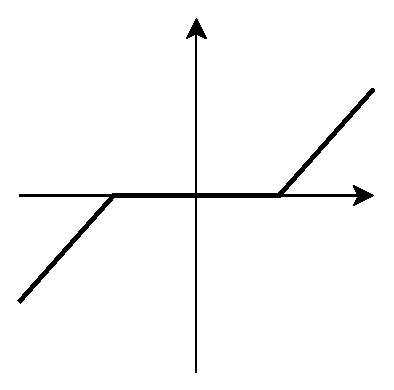
\includegraphics{func_nosense} &
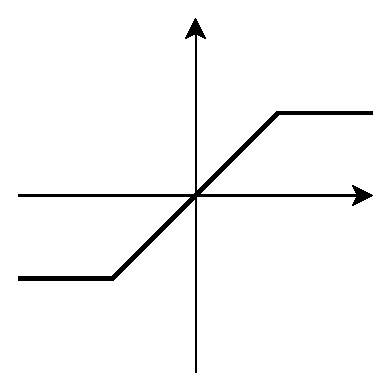
\includegraphics{func_saturat} \\
а) Зона нечувствительности ({\tt nosense})& б) Насыщение ({\tt saturat}) \\
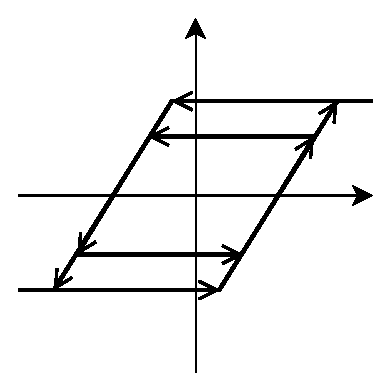
\includegraphics{func_luft} &
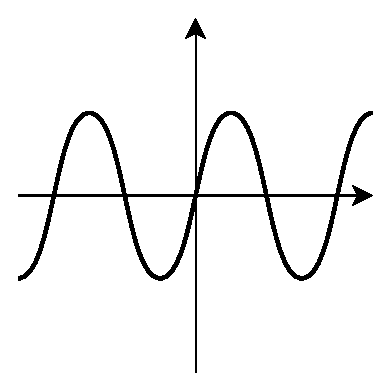
\includegraphics{func_sine} \\
в) Люфт ({\tt luft}) & г) Синус ({\tt sine}) \\
\end{tabular}
\caption{Реализованные в пакете нелинейные звенья.}
\label{fig:nonlinear_functions}
\end{figure}

Количество нелинейных звеньев в пакете намеренно сделано небольшим.
Расширение списка нелинейных звеньев может быть предложено студентам в
качестве одного из направлений учебно-научной работы.

Нелинейные звенья могут комбинироваться с линейными в любом порядке.
Пример файла, задающего функцию объекта в виде инерционного звена
первого порядка $I^*(z)=\frac{1.6z}{z-0.7}$ с зоной
нечувствительности, приводится ниже:

\begin{verbatim}
;NeuCon combined function 1.0
[CombinedFunction main]
TransferFunction inert
CustomFunction deadzone

[CustomFunction deadzone]
; Extension:   .so/.dll depending the OS
file    nosense
;HalfWidth Gain
options 0.5 2
;Initial vector (may be empty)
initial

[TransferFunction inert]
polyfrac 0
 1.6 0 /  1 -0.7
\end{verbatim}

Краткое описание формата файла комбинированной функции приводится в
\tablref{tabl:cof_syntax}.

\begin{table}[ht]
\centering
\caption{Описание формата файла задания комбинированной функции.}
\label{tabl:cof_syntax}
\begin{tabular}{|c|l|p{8cm}|}
\hline
Правило & Синтаксис & Семантика \\
\hline
1 & \tt ;NeuCon combined function 1.0 & Служебный комментарий в первой строке файла \\
2 & \tt ;                    & Признак комментария до конца строки \\
3 & \tt [CombinedFunction \em Имя \tt] & Признак начала описания комбинированной функции, действующей в порядке перечисления \\
4 & \tt TransferFunction \em Имя & Ссылка на линейную функцию {\em Имя} \\
5 & \tt CustomFunction \em Имя & Ссылка на пользовательскую функцию {\em Имя} \\
6 & \tt [TransferFunction \em Имя \tt] & Признак начала описания передаточной функции (см. \tablref{tabl:tf_syntax})\\
7 & \tt [CustomFunction \em Имя \tt] & Признак начала описания пользовательской функции \\
8 & \tt file \em ИмяФайла & Имя файла без расширения ({\tt .so} или {\tt.dll}) с библиотекой, реализующей функцию \\
9 & \tt options \em Параметры & Перечень числовых параметров функции (через пробел) \\
10 & \tt initial \em Инициализация & Перечень чисел для инициализации начального состояния функции (через пробел) \\
\hline
\end{tabular}
\end{table}


%fil% \subsubsection{Нестационарные элементы моделирования}
\paragraph{Нестационарные элементы моделирования}

Нестационарное поведение объектов моделирования реализуется в
программном пакете двумя способами:
\begin{enumerate}
\item с помощью специально запрограммированного звена, обладающего
  нестационарными свойствами;
\item заданием списка функций и времени переключения с одной функции
  на другую.
\end{enumerate}

Первый способ более общий.  Он позволяет реализовать произвольное
поведение объекта, например, плавное изменение параметров.  Однако он
требует запрограммировать необходимые действия и скомпилировать
полученный программный модуль в виде внешней пользовательской
библиотеки, что не всегда удобно и ведет к дополнительному расходу
времени.

Второй способ позволяет описать в текстовом файле комбинированной
функции правило, по которому будет изменяться функция объекта.
Правило задается перечнем функций и периодами времени, в которые эти
функции реализуют поведение объекта.  В целом, для функций $g_i()$ и
моментов времени $t_i$ правило вычисления действующей функции объекта
описывается формулой:

$$
y=\left\{
\begin{array}{ll}
  g_1(t,x), & 0\le t < t_1\\
  g_2(t,x), & t_1\le t < t_2\\
  ... & \\
  g_l(t,x) & t \ge t_l
\end{array}\right.
$$

\noindent где все $t_i$ кратны шагу дискретизации времен в сеансе
моделирования.

Например, если надо запрограммировать изменение коэффициента усиления
c 1.5 на 3.4 в момент времени $t=500$, это можно описать в файле
следующей комбинированной функцией:

\begin{verbatim}
;NeuCon combined function 1.0
[CombinedFunction main]
TransferFunction k1 0 500
TransferFunction k2 500 -1

[TransferFunction k1]
polyfrac 0
 1.5 /  1

[TransferFunction k2]
polyfrac 0
 3.4 /  1
\end{verbatim}

%\subsubsection{Нейронные сети и методы их обучения}
%fil% \subsubsection{Моделирование динамических систем}
\paragraph{Моделирование динамических систем}

Задача моделирования динамической системы в дискретном времени
заключается в упорядоченной активации взаимосвязанных функциональных
блоковб моделирующих поведение отдельных элементов системы и передачи
порций данных между ними.  Типичной динамической системой является
контур управления с обратной связью.  Входными данными для этой
системы является внешний сигнал уставки.  С целью имитации реальных
условий в контуре присутствует аддитивная помеха в канале наблюдения
объекта.  Таким образом, помеху также можно отнести к внешним
сигналам.  Остальные сигналы производятся функциональными блоками в
процессе моделирования.

Задачей программы моделирования является правильная коммутация
выходных сигналов одних функциональных блоков на вход других.  Если
принять функциональный блок за узел, а передачу данных между блоками
--- за направленное ребро, то модель динамической системы может быть
представлена как ориентированный граф.  Для обеспечения правильных
результатов моделирования и, учитывая, что оно происходит в дискретном
времени, функциональный блок должен вырабатывать порцию выходных
данных только если у него есть для этого данные на входах.  Важной
особенностью является однократное использование каждой порции данных
на входе любого блока.  Таким образом, порции данных также являются
синхронизирующими метками.  Графы описанного типа относятся к классу
сетей Петри \cite{petri_network}\cite{makloh01}, применяемых в моделировании
динамических систем различных типов.

Помимо моделирования контура управления с обратной связью описанный
аппарат сетей Петри хорошо подходит для реализации различных схем
обучения нейронных сетей как в контуре управления, так и вне его.  При
этом естественным образом выражаются многие аспекты алгоритмов
обучения нейронных сетей, такие как последовательное и пакетное
обучение, задание порядка обучающих пар, компоновка обучающих пар для
реализации нейросетевых моделей авторегрессии и скользящего среднего.
Таким образом, для решения всех основных задач, перечисленных в
п.\ref{main_tasks}, можно воспользоваться одним и тем же аппаратом.

Особенностью динамических систем, моделируемых в программном пакете,
является наличие обратной связи в контуре управления, то есть,
ориентированный граф содержит цикл.  В рамках описанного формального
подхода наличие цикла мешает начать моделирование контура управления,
поскольку в начальный момент времени для расчета ошибки управления
необходимо из уставки вычесть наблюденный на предыдущем шаге выход
объекта управления, в том время как предыдущего шага ещё нет.  Для
разрешения этой проблемы в одном из ребер цикла графа вводится
специальная порция данных --- так называемый стартёр.  Эта порция
данных представляет собой начальные условия, позволяющие запустить
нормальное функционирование контура обратной связи.

В объектно-ориентированной библиотеке {\tt NeuArch} реализован набор
унифицированных классов, позволяющих организовать в программе сеть
Петри произвольной архитектуры (не более чем с одним циклом) из
функциональных блоков, интерфейс взаимодействия между которыми
абстрагирован.  Каждый блок может иметь произвольное число входов и
выходов, причем единицей передаваемых данных является вектор ---
массив чисел зафиксированной на этапе создания сети размерности.
Имеются два основных правила, которому должны следовать все прикладные
блоки сети Петри:
\begin{enumerate}
\item функция блока активируется только если на всех входах есть
  свежие данные;
\item функция блока всегда производит свежие данные на всех выходах.
\end{enumerate}

Библиотека позволяет реализовать и более сложную логику поведения
функциональных блоков, однако пользоваться этими возможностями следует
осторожно во избежание неожиданных эффектов при моделировании.

%fil% \subsubsection{Объекты для моделирования дискретных динамических систем}

Для построения основных прикладных вычислительных программ библиотека
предлагает широкий спектр функциональных блоков, имеющих
вычислительное, коммутационное и системное назначение
(\tablref{tabl:pn_objects}).
%  Для удобства разработки программ с
%сетями Петри и лучшего понимания их функционирования разработана
%система графических обозначений для некоторого количества
%специфических блоков.  Эти блоки перечислены на~\figref{fig:pn_icons}.

\begin{table}
\centering
\caption{Функциональные блоки для построения сети Петри.}
\label{tabl:pn_objects}
\begin{tabular}{|l|l|p{11.5cm}|}
\hline
$\mathrm N^0$ & Класс \tt C++ & Назначение \\
\hline
1  & \tt NaPNActor & Заданное действие по приходу данных. \\
2  & \tt NaPNBus2i1o & Склейка двух векторных входов в один векторный выход суммарной размерности. \\
3  & \tt NaPNCheckPoint & Транзитное звено с протоколированием потока данных в заданный файл. \\
4  & \tt NaPNComparator & Вычисление разности двух входных векторов. \\
5  & \tt NaPNConstGen & Генератор постоянного значения на выходе. \\
6  & \tt NaPNCuSum & Обнаружение разладки с помощью АКС. \\
7  & \tt NaPNDelay & Формирование по входу $x_k$ выхода $x_k,x_{k-1},...,x_{k-D}$, где $D$ --- заданная задержка. \\
8  & \tt NaPNDerivative & Вычисление дискретной производной. \\
9  & \tt NaPNFetcher & Выборка некоторых элементов из входного вектора. \\
10 & \tt NaPNFill & Выдача заданного значения в качестве нескольких первых порций данных. \\
11 & \tt NaPNFileInput & Чтение данных из файла. \\
12 & \tt NaPNFileOutput & Запись данных в файл. \\
13 & \tt NaPNGenerator & Генерировать выходные значения с помощью заданной функции. \\
14 & \tt NaPNLogicalAND & Логическое ``И'' над входами.  Положительное значение --- истина ($+1$), нулевое или отрицательное --- ложь ($0$). \\
15 & \tt NaPNNNUnit & Вычисление выхода по входу нейронной сетью. \\
16 & \tt NaPNQueueInput & Чтение данных из внешнего источника общего вида. \\
17 & \tt NaPNQueueOutput & Запись данных во внешний приемник общего вида. \\
18 & \tt NaPNRandomGen & Генерация псевдослучайной последовательности. \\
19 & \tt NaPNSkip & Пропуск указанного количества первых порций данных. \\
20 & \tt NaPNStatistics & Расчет статистических параметров входных данных нарастающим итогом. \\
21 & \tt NaPNSum & Суммирование входов. \\
22 & \tt NaPNSwapper & Управляемый коммутатор прямого или перекрестного отображения входов на выходы. \\
23 & \tt NaPNSwitcher & Управляемый коммутатор направления первого или второго входа на выход. \\
24 & \tt NaPNTeacher & Обучение нейронной сети. \\
25 & \tt NaPNTrainDataGath & Сбор обучающих данных по критерию минимальной плотности покрытия. \\
26 & \tt NaPNTimeDepend & Счетчик дискретного времени. \\
27 & \tt NaPNTimer & Счетчик тактов моделирования. \\
28 & \tt NaPNTransfer & Передаточная функция. \\
29 & \tt NaPNTrigger & Управляемый пропуск порций данных. \\
30 & \tt NaPNWatcher & Заданное действие над порцией данных.\\
\hline
\end{tabular}
\end{table}

%\begin{figure}[h]
%\centering
%\begin{tabular}{cс}
%\hbox{\input{Bus2i1o.pic}} & \hbox{\input{Comparator.pic}} \\
%а) & б)\\
%\end{tabular}
%\caption{Графические обозначения некоторых функциональных блоков: (а)
%         и рабочего функционирования (б).}
%\label{fig:pn_icons}
%\end{figure}

%Bus2i1o.pic
%Comparator.pic
%Summator.pic
%Delay.pic
%Delta.pic
%FetcherLtoR.pic
%FileIO.pic
%LAnd.pic
%QueueL.pic
%QueueR.pic
%RandomNormal.pic
%RandomUniform.pic
%Skip.pic
%Statistics.pic
%SwitcherPM.pic
%TriggerLtoR.pic
%NNUnit.pic
%Teacher.pic
%
%\subsubsection{Формализм для графического представления динамических моделей}
%\subsubsection{Пример: дообучение нейросетевого регулятора в контуре}
%\subsubsection{Пример: моделирование САУ и обнаружение разладки}


%%%%%%%%%%%%%%%%%%%%%%%%%%%%%%%%%%%%
\section{���������� ������ � ����� ������������ �����}
% -*-coding: utf-8;-*-
%\section{Применение пакета в курсе лабораторных работ}

На базе разработанного программного пакета моделирования и
конструирования традиционных и нейросетевых систем управления был
разработан курс лабораторных работ.  Этот курс демонстрирует, с одной
стороны, возможности применения нейронных сетей для решения различных
задач автоматического управления, с другой стороны, возможности
программного пакета для моделирования САУ и обучения нейронных сетей.

%\subsection{Интеграция в учебный процесс}

Разрабатываемый курс лабораторных работ предназначен для расширения
существующего курса, посвященного применению искусственных нейронных
сетей в целом.  В рамках имеющихся ограничений по времени на
нейросетевые системы управления выделено три практических занятия
длительностью 3--4 часа каждое.  Представляется оптимальным
скомпоновать учебный материал в занятия по следующим темам:

\begin{itemize}
\item Синтез нейросетевого оптимального регулятора.
\item Сравнительный анализ нейросетевого, винеровского и ПИД регуляторов.
\item Нейросетевое управление нестационарным объектом.
\end{itemize}

Первая лабораторная работа посвящается методике замены регулятора в
существующей системе управления на нейросетевой.  Для этого необходимо
провести моделирование и собрать данные для начального обучения
нейросетевого регулятора и модели объекта.  После этого требуется
настроить нейронные сети регулятора и модели объекта.  Предварительно
настроенный регулятор включается в САУ на место исходного и с помощью
модели объекта в процессе работы подстраивается для минимизации ошибки
управления.

В рамках второй работы требуется сравнить настроенный нейросетевой
регулятор с винеровским оптимальным и ПИД регулятором в различных
условиях, как номинальных (используемых при настройке), так и
отличающихся от них.  В частности, следует провести моделирование с
разными типами сигналов уставки и интенсивностью помехи,
экспериментально исследовать зависимость качества управления от
частоты, определить, насколько чувствителен регулятор к точности
задания параметров объекта управления.

Третья лабораторная работа посвящена задаче нейросетевого управления
нестационарным объектом.  Она включает настройку системы обнаружения
разладки с помощью нейросетевой модели и алгоритма кумулятивных сумм
(АКС), сбор данных и подстройку с их помощью модели объекта
управления, а также подстройку нейросетевого регулятора в контуре.

Тематика лабораторных работ достаточно разнообразна.  В частности,
рассматриваются как конструкторские (синтез элементов САУ, подключение
АКС), так и исследовательские задачи (выбор оптимальной архитектуры
нейросети, сравнение различных регуляторов).  Сопоставление с
линейными регуляторами, в том числе, с винеровским оптимальным,
связывает материал курса с классической теорией автоматического
управления.  Использование АКС для обнаружения разладки демонстрирует
возможность совместного использования нейросетевых и традиционных
алгоритмов.

%\subsection{Дидактические аспекты}

Успешное выполнение практической работы требует от студента следующих
видов деятельности:

\begin{itemize}

\item изучение теоретических основ нейронных сетей;

\item освоение программного комплекса;

\item подготовку отчета.

\end{itemize}

Материал, вошедший в лабораторные работы, подразумевает, что помимо
теоретических знаний лекционной части курса студент обладает знаниями
по математической статистике, теории функций комплексного переменного
и линейной теории автоматического управления (для детерминированных и
стохастических сигналов).

В результате выполнения практических работ студент должен изучить:
\begin{itemize}

\item Архитектуру нейронных сетей прямого распространения.

\item Способы реализации нейронными сетями динамических свойств
  элементов системы автоматического управления ($\{{e_k,r_k}\}$,
  $\{e_k,e_{k-1},...\}$, $\{u_k,u_{k-1},...y_k,y_{k-1},...\}$).

\item Влияние выбранного критерия качества управления, используемого
  при настройке регулятора, на функционирование САУ в условиях,
  приближенных к реальным (помеха, неточная параметризация сигналов и
  объекта управления, нестационарность).

\item Метод обратного распространения ошибки и его применение при
  синтезе элементов нейросетевой системы управления (начальная
  настройка и подстройка в контуре нейросетевого регулятора, настройка
  нейросетевой модели объекта управления).

\item Роль нейросетевой модели объекта при синтезе нейросетевого
  регулятора и при обнаружении разладки.

\item Влияние обучающих и контрольных данных на свойства обученной
  нейронной сети (область определения и область значений нейросети).

\item Основные свойства нейросетевых регуляторов и их отличия от
  линейных регуляторов (частотная характеристика, зависимость от
  уровня сигналов, устойчивость, адаптированность к нелинейным
  объектам и пр.).

\item Методы нейросетевого управления нестационарным объектом и их
  особенности (быстродействие, ресурсоемкость, устойчивость).

\end{itemize}


%%%%%%%%%%%%%%%%%%%%%%%%%%%%%%%%%%%%
\section{�������� ������������ �����}
% -*-coding: cp1251;-*-
%%%%%%%%%%%%%%%%%%%%%%%%%%%%%%%%%%%%%%%%%%%%%%%%%%%%%%%%%%%%%%%%%%%%%%%%%%%%%%
%\section{�������� ������������ �����}

%%%%%%%%%%%%%%%%%%%%%%%%%%
% ������������ ������ �1 %
%%%%%%%%%%%%%%%%%%%%%%%%%%
\subsection{������ ������������� ����������}

%fil% \subsubsection{���� ������}
\paragraph{���� ������}

������������ ������ ��������� ������ ������� �������������
������������ ����������.  � ��� ��������� �������� ����������
��������� ����� � �������� ���������� � ������ ������� ����������.
����������� ������� ����������� ��������� ���� �� �������� � ��������
��������.  ���������� ��� ������������ � ����������� ������������
�������.

%fil% \subsubsection{���������� ������}
\paragraph{���������� ������}

������� ������� ���������� � �������� ������.  � ������� ����������
���� ����������� ���� � ���� ����������� �����.  ��������, ��� �
������ ���������� ������� ��������� ������.  ���� ��������������
������ ������� �������.  ���������� �������� ��������� �� ������������
� ������������ �������� ������ ����������.

��� �������� ��������� ������ � � ����� ������������ ��������� �
��������� ������������ � �������� ������� ���������� � ����������
������� �������� ������, ���� �������� ������� ����� �� ������������ �
������ ������ ������������ ������� � ����������� ����������.

� �������� ���������� ������������� ������ ������� ����������� �������
����������� ��������� ���� (���������� �����, ������������� �������� �
���) �� �������� �������� � ����������� ��������.

%fil% \subsubsection{��������}
\paragraph{��������}

��������� �������� ������ ������ ����� ����������, ������� ������
��������� ������� ����������, ������� � ������.

%fil% \subsubsection{���� ������}
\paragraph{���� ������}

���� ��������������� ��������� ��������� ���������:
\begin{enumerate}
\item ������������� ��� � �������� ����������� � ������� � ����� �����
  ������ ��� �������� ��������� �����.
\item ������� ����������� ������������ ������ ������� ����������.
\item �������� ������������ ������ ������������ ������������ ������
  ������� ����������.
\item ��������� ��� ���������� ������ ��� ������ ���������� ���������
  �����.  ������� ��������� �� �������� ������ ������������ ��
  �������� �������.
\item ������� ����������� ������������� ����������.
\item �������� ������������� ���������� ���������������� �������
  ��������� ��� ������� ����������.
\item ��������� ��� ���������� ������ ��� ������ ���������� ���������
  �����.  ������� ��������� �� �������� ������ �������� �� ��������
  �������.
\item ������ ��������� ���������� ������������ � ������� ���������� �
  ��������� ������� ��� ��������� � ������� ������������ ������.
\item ������������� ��� � ��������� ������������ ����������� � �������
  � ����� ��������� ��� � ��������.
\end{enumerate}

%fil% \subsubsection{������ ������}
%\paragraph{������ ������}

%\subparagraph{�������� �������� ������� ����������}
%\begin{itemize}
%\item ������ ����������: $P^*(z)=?$
%\item ����������� ������ �������: $R^*(z)=?$
%\item ����������� ������ ������: $N^*(z)=?$
%\item ���������: $C^*(z)=?$
%\end{itemize}

%�������� ���������� ������ ���������� � ������� (�������, �����������
%����� �������, ������).  �������� --- ���������� � ������ ����������.

%���������� ������ ���������� �� ������� ��������� ����.

%����� � ��������� ������������� $u\times y$ ��������� � �����������
%������� ����� ��������� ��--� ��� �������.

%�������� 3-� ������ ���������� ��--� � ����� ������ ������ �� ��������
%��������� ������� ����������.  �������� ������� �������� � �����������
%�������� ������ ��������.

%����� � ��������� ������������� $r\times e$ ��������� � �����������
%������� ����� ��������� ��--� ��� �������.

%�������� 3-� ������ ���������� ��--� � ����� ������ ������ �� ��������
%��������� ��������� ����������.  �������� ������� �������� �
%����������� �������� ������ ��������.

%������������ ������ ��--� � �������.  ����������.

%������ ��� � �������.  ������ ������.  ������������ ������ ��� �
%�������.  ����������.


%%%%%%%%%%%%%%%%%%%%%%%%%%
% ������������ ������ �2 %
%%%%%%%%%%%%%%%%%%%%%%%%%%
\subsection{��������� �������������, ������������ ������������ � ��� ����������}

%fil% \subsubsection{���� ������}
\paragraph{���� ������}

������ ��������� ������������ ������� ������������� ���������� �
��������� � ��������� ������������: ������������� � ������
������������ � ������������ ���������� ��� ����������� � �����������
--- ����������� � ������ �������� ���.  ��������� �����������
���������� � ��������� �������� �� ������ �������������
(�������������������� ������) � �������������� (������������ ������)
���������.

%fil% \subsubsection{���������� ������}
\paragraph{���������� ������}

������� ������� ���������� � �������� ������ � �������� ��������
����������.  �������������� ��������� ������� � ������ ������.  ���
������� ������������� ��� ���������, ����������� ����������� ���������
\footnote{�������� ������ ������ ����� ���, ����������� �������������
  ��������� ������������ ������������ ������������ ����������} �
������������ ����������� ���������, ��������, ���������� �� �����
������ ������������ ������.

��������� ����������� ������� ��������� ������ �� ������������ ���
�������� ���������� �� ���������� ������� ��������� ���������.
���������� �������� ���������� �������� ������������ �� ������
����������������� � �������������������� ������.

��������� ���������������� ����������� ��������� ���� �����
����������� � ����������� ��������, �� ������ ����� ������� �������
(�����������, �������������, ��������������), � ����� � ��������,
�������� �� �����������: ���� ��������� ������� ����������, ������� �
������ (����������, ����������� �������, ���������� ������� ������,
``�������'' ������).  ���������������� ���������� ����������� ��������
���������� �� �������, ������� �� ���� ������� ������������� �������.

%fil% \subsubsection{��������}
\paragraph{��������}

������ ������ ����� ����������� �� ��������� �������� ��� (���������
������� ����������, ������� � ������), � ����� �� ������ �������������, �������
������� ��������.

%fil% \subsubsection{���� ������}
\paragraph{���� ������}

������ ����� ����� ������ ������������� ����������� �� ������ �������
����� ������������� ��� ������� �� ���� ����� �����������.  ����� ����
���������� ����������� ������� ������� � ������, � ����� ����������
��������� ������� ���������� ��������� �������.

\begin{enumerate}
\item ����������� �������������� ������� � ������, ����������� ������
  ����������.
\item ������� --- ������ � ������������� ��������, ����������� ���
  ���������� ����������� ��������.  ������ --- �����������.  ������
  ���������� --- �����������.
\item ������� --- ���������.  ������ --- �����������.  ������
  ���������� --- �����������.  ��������� ��� ���������� ���������
  ������ ������� , ������� ������� ���������.
\item �������������� �������, �������� �� ����������� � ����������,
  �������� ����������� � �����������.  ����������� ������.  ������
  ���������� --- �����������.
\item �������������� �������, �������� �� ����������� � ����������, �
  ��� ���� ����������� �����������.  ����������� ������.  ������
  ���������� --- �����������.
\item ����������� �������������� �������.  ������ --- ����� ��� �
  �������������� � ��� ���� ������, ��� �����������.  ������
  ���������� --- �����������.
\item ����������� �������������� �������.  ������ --- ``�������'' ���.
  ������ ���������� --- �����������.
\item ����������� �������������� ������� � ������.  ��������� �������
  ���������� ���������� �� �����������.
\item ����������� �������������� ������� � ������.  ��� �������
  ���������� ���������� �� ������������.
\end{enumerate}

%fil% \subsubsection{������ ������}
%\paragraph{������ ������}


%%%%%%%%%%%%%%%%%%%%%%%%%%
% ������������ ������ �3 %
%%%%%%%%%%%%%%%%%%%%%%%%%%
\subsection{������������ ���������� �������������� ��������}

%fil% \subsubsection{���� ������}
\paragraph{���� ������}

������������ ������ �������� �� ���������� ������������ �������
���������� �������������� ��������.  ��������������� �������
����������� �������� � ������� ������������ ������ ������� � ���������
������������ ����, ����� ��������� ������ � ���������
���������� � �������.

%fil% \subsubsection{���������� ������}
\paragraph{���������� ������}

��������������� ������ ��������� ������������� ���������� ���
����������� ��������� � ��������� ������� ����������.  �������, ���
��������� ���������� ���������� ����� � ����������.  ������� � ������
�������� ��������������� � �� ��������� ����� �������.

����� ������������� ���������� ������� ����� ������������ ������
������� ����������, ���������� ����������� � �������� � ��������
������������ ��� ������.  �������� ������������ � ������ ��������
������� �������������.  ��� ������������ ����� ��������� ���� ������
��������� ������������� ���� ��������, �� ����, ��������� �������
����������.  ��--� � ��--� �������� � ���� ������ ������������ ������.

��� ����������� �������� �� ��������� ������ ������������� �����������
�������� ������������ ����, ������������� � ����� ����������
���������� ����� ������������ �������� ������� ������������ ���
����������� �������� � ������������� �������� ������� ����� �������
���������.  ��������� ������������ ����������� ��� �������� �����
(�������� �������) � ����������� ��������.

����� ����������� �������� ������������ �������� ����� ������ ���
��������� ������ ������� ����������.  ������������ ������ �������
�������������� ��� ������� � ����� ���������� �������� � ��������
���������� �������� ��������� ��--� � ������� ����������.  ���
������������ ������������� ������ ���������� �������� ���������
�����������.

%fil% \subsubsection{��������}
\paragraph{��������}

��������� �������� ������� ����� ���� ������������ �� ���� ���������
�������� ����������, �������� ������������ ����������� � ����������
������� � ������.

%fil% \subsubsection{���� ������}
\paragraph{���� ������}

\begin{enumerate}
\item ��������� ���������� ��� ��� ����������� ��������.  �������
  ����������� �������� � ����� ����������� ���������������� ��
  ��������� ���������� �������� �������� ������� ������������ �
  �������� ������� ����� ������� ���������.
\item ������������� ��� � ���������� ���������� ������� ���������� �
  �������� ������ �������.  ����������� ����� �������� � ������� ���.
\item ���� ������ ��� ��������� ������������ ������ �������
  ����������.
\item �������� ������������ ������ ������������ ������������ ������
  ������� ����������.
\item ��������� ������� ��������� ��--� � ������� �����������������
  ������������ ������.  ����������� ��������� �� ����������
  ����������� ������ ������ ����������.
\item ������������� ��� � ����� ��--� � ������� � ����� ��������� ���
  � ��������.
\end{enumerate}

%fil% \subsubsection{������ ������}
%\paragraph{������ ������}


%%%%%%%%%%%%%%%%%%%%%%%%%%%%%%%%%%%%
\section{������}
% -*-coding: utf-8;-*-
%%%%%%%%%%%%%%%%%%%%%%%%%%%%%%%%%%%%%%%%%%%%%%%%%%%%%%%%%%%%%%%%%%%%%%%%%%%%%%

\begin{enumerate}
\item Разработан интерактивный программный комплекс для моделирования
  одноконтурных систем автоматического управления в дискретном времени
  с возможностью использования линейных, нелинейных и нестационарных
  объектов.  В пакете имеются развитые средства для синтеза
  нейросетевого регулятора и нейросетевой модели объекта управления
  для стационарного и нестационарного объектов, а также возможность
  моделирования контура управления с включенными нейросетевыми
  элементами.
\item Предложена методика использования программного комплекса в
  учебном процессе на инженерных специальностях высших учебных
  заведений для практических занятий и научных исследований в курсах
  по нейронным сетям и по системам управления.
\item Разработан курс из трех лабораторных работ по применению
  нейронных сетей в системах управления, включающий освоение
  студентами методов синтеза нейросетевых систем управления
  стационарными и нестационарными объектами, а также сопоставление
  нейросетевого, винеровского оптимального и ПИД регулятора в
  различных условиях.
\end{enumerate}



% Заключение
\chapter*{Заключение}
\addcontentsline{toc}{chapter}{Заключение}

% Библиография
\bibliography{Bibliogr}

% Приложения
%\appendix

% Приложение 1 - Эксперименты
%\section{Сравнительные эксперименты с ПИД, Винеровским и нейросетевым
%         оптимальными регуляторами}
%% ���������� 1 - ������������ �� ������������ ��������������� ����������
% � ������������ ������

%%%%%%%%%%%%%%%%%%%%%%%%%%%%%%%%%%%%%%%%%%%%%%%%%%%%%%%%%%%%%%%%%

� ��������� ���������� ���������� ��������� �������� ������������� �
�� ����������.  � ������������� ��������� ������� ���, �����������
����������� � ������������ ����������� ����������.  ���� �������������
����������� � ��������� ������������ ������������� ��\-����������
���������� � �������� ������������ ������ �� ��������� � �������������
���������� ��������� ����������.\label{appendix1}

����������� ��������� �������� �� ���� ������������� ������ ����
�����������.  ����������� ������ ��������� ������� --- �����������
����� 1-�� �������.  ������� ������ ��� ����� ��� ���������
������������ ���������.  ������� ������ ��������� ������� � ���, ���,
��-������, ��� ������ ����� ������������ �� �������� ��� ����������
����������� � ������� ��� �������������, ��-������, � ����� �������
������� ��������� ��� ������������ ������������ ������� ����������
���������� ����������, ��� � ������������ ������� ��������� ���
���������� ����������.

��������� ��� ���������� ����������� �������� � ����������� ��
����������� ������� ��� ���������� ������.  ������������� ���������
���������� ���� ��������� �� ������ ������������� ������������, �
������������ ��������������� ��� ������� �� ��������� � ���
�������������.

������ ������������ ���������� ���������� ������������.
��������������� ��������� ��������, ����� ��������� �������� � �������
���������� �������� �����.  � ���������� ��������� ����� ������� �
��������� ������������.  ����� ����, ��� ������� � ������� ������
���������� ������������� ������������� ������, ��� ��� �������.
�������, �������� ����������� ������� �������������, � �������������
�������������� ������� ������� � ������� ����������.

������ ������������� ������������ ���������� (���) ���������� �
����������� �������� ��� ������������� ��������� ���������� ��
��������, ���������� � �.\ref{noc_synthesis_method}.

\section{������ ���������� ������� �������}
% ������ ���������� ������� �������
\label{W1op_case}

�������, ���������������� �������� ����������� ������, ��������
���������� ��������� �� ������ �������� �������� ����������.  �
���������, ����� ����� ������� ������� � ������������ ��� ���������
������������� ������ ������������� �������� ����������� �������.

\subsection{����������� �������}%
\label{W1op_nominal_cond}

\begin{itemize}

\item
����������� ������ �������:
$R^*_1(z)=\mathcal{Z}\Bigl\{\displaystyle\frac{2.5}{1+4s}\Bigr\}
         =\displaystyle\frac{0.625z}{z-0.7788}$

\item
����������� ������ ������:
$N^*_1(z)=0.1$

\item
����������� ����������� ������:
$W^*_1(z)=\displaystyle\frac{0.9754z}{z-0.0192}$

������������������ ������ ���������� $\MSE_{min}=0.0098$

\item
������ ����������:
$P^*_1(z)=\displaystyle\frac{3z}{z-0.8}$

\item
����������� ����������� ���������:
$C^*_{WOC_1}=\displaystyle\frac{0.3251z-0.2601}{z-0.9946}$

\item
�������� ��� ��������� (��. \figref{fig:dw1op_pid_step}):
$$
C^*_{PID_1}(z)=0.2 +
             0.08\displaystyle\frac{z}{z-1} +
             0.05\displaystyle\frac{z^2-2z+1}{z(z-1)}
$$

\end{itemize}

\begin{figure}[h]
\centering
\hbox{\psfig{figure=dw1op_pid_step.ps,angle=270,width=0.8\textwidth,%
             height=0.35\textheight}}
\caption{���������� �������������� ���������� ������� ��� ��� ����������.}
\label{fig:dw1op_pid_step}
\end{figure}

\subsection{����������� � ��������� �������� ��--�}%
\label{W1op_NNP_descr}

\begin{itemize}

\item
����������� ��--�: $\NN^o_{1+1,1}$

\item
������������ �������� ��������: $\eta_h=0.01$, $\eta_o=0.001$

\item
��������� �������: ����� $L=1000$, ��������� �������� ��������:
$u=[-0.80, 0.80]$, $y=[-2.89, 3.88]$
%$u=[-0.7997, 0.8008]$, $y=[-2.8877, 3.8840]$

\item
����������� �������: ����� $L=1000$, ��������� �������� ��������:
$u=[-0.80, 0.72]$, $y=[-4.02, 4.16]$
%$u=[-0.8010, 0.7169]$, $y=[-4.0234, 4.1574]$

\item
�������� � ������� 95 ���� �� ������ ����� $\MSE$ �� ����������� �������.

\end{itemize}

\subsection{����������� � ��������� ���������������� �������� ��--�}%
\label{W1op_NNCpre_descr}

\begin{itemize}

\item
����������� ��--P: $\NN^o_{1+1,1}$

\item
������������ �������� ��������: $\eta_h=0.05$, $\eta_o=0.005$

\item
��������� �������: ����� $L=500$, ��������� �������� ��������:
$r=[-2.62, 2.59]$, $e=[-1.94, 1.73]$, $u=[-0.66, 0.58]$
%$r=[-2.6234, 2.5899]$, $e=[-1.9396, 1.7348]$, $u=[-0.6638, 0.5822]$

\item
����������� �������: ����� $L=500$, ��������� �������� ��������:
$r=[-2.58, 3.22]$, $e=[-2.25, 2.09]$, $u=[-0.67, 0.80]$
%$r=[-2.5778, 3.2184]$, $e=[-2.2461, 2.0882]$, $u=[-0.6730, 0.7979]$

\item
�������� � ������� 10 ���� �� �������� �������� ���������� ������ ��
����������� ������� ������ $10^{-5}$.

\end{itemize}

\subsection{��������� ���������� ��--� � �������}%
\label{W1op_NNCfin_descr}

\begin{itemize}

\item
������������ �������� ��������: $\eta_h=0.0001$, $\eta_o=0.00005$

\item
������������ ����� $L=300$

\item
�������� �������� � ����������� �������� �������� $\MSE$
�������������� �� ���� 50 ����.  ��� �������� �������������
������������ �������� �����, ���������� �� �������
(\cite[�.~797--799]{aivmhit98}).  ������� ���������� ��������
$\alpha=5\%$.

\item
�������� ����������� �������� �������� $\MSE$ ��������� �������� ��
����� �� ����� ����, �� ����, �������� ���� ����������� ����� 250
��������� ����.

\end{itemize}

\subsection{������������� �������}%
\label{W1op_differ_cond}

\begin{description}

\item[$E_{r-}$:]
����������� �������� �������: $R^*_1(z)=\displaystyle\frac{0.313z}{z-0.7788}$

\item[$E_{r+}$:]
����������� �������� �������: $R^*_1(z)=\displaystyle\frac{1.250z}{z-0.7788}$

\item[$E_{n-}$:]
����������� �������� ������: $N^*_1(z)=0.05$

\item[$E_{n+}$:]
����������� �������� ������: $N^*_1(z)=0.2$

\item[$E_m$:]
������� ������������ ����� ������������������ ������������� ���������
���������� 1, �������� 40 � ������������� �������� 20 ����������
�������� �������.  ����� ����� ���������� ���� ��������� 150
���������� �������� �������.

\item[$E_s$:]
������� ������������ ����� ������������� ������ ��������� 1 � ��������
�������.  ��� ������������ �������� ���������� �� ��������� ��������
���� ��������� ������������ � �������� �������������� ������� �� 2 ��
50 ���������� �������� �������.  ����� ����� ���������� ���� ����
����� 500 ���������� �������� �������.  ������������ ����������� �
������� ������� ��� ����, ����� �������� ��������� ��� �����������
�������� ���������� �� �������.

\item[$E_p$:]
������ ���������� � ����������� �� ��������� � �����������
��������������: $P^*_{1'}(z)=\displaystyle\frac{3z}{z-0.4}$

\end{description}

\subsection{���������� �������������}%
\label{W1op_results}

���������� ������������ �� ����� � ��� �� ������������ ������� �������
� ������.  ����� ��������� ���������� ���� ���������� 10000 ����������
�������� ������� �� ���� ������������� ����� $E_m$ � $E_s$.
���������� ��������� �������� ���������� �� ������������������ ������
� �� ������������� ����������������� ���������� �
\tablref{tabl:dw1op_wpn_diff_env}.

\begin{table}
\centering
\caption{�������� ���������� �������� $P^*_1$ ���������� ������������
         � ��������� �������� ������������}
\label{tabl:dw1op_wpn_diff_env}
\begin{tabular}{|l|l|l|l|l|l|l|}
\hline
�������      & \multicolumn{3}{|c|}{$\MSE$} & \multicolumn{3}{|c|}{$\Emax$} \\
\cline{2-7}
������������ & $C^*_{PID_1}$ & $C^*_{WOC_1}$ & $\NN^p_{r+e,1}$ &
               $C^*_{PID_1}$ & $C^*_{WOC_1}$ & $\NN^p_{r+e,1}$ \\
\hline
$E_0$        & 0.0201 & 0.0098 & 0.0063
             & 3.0906 & 2.9684 & 2.9618 \\
$E_{r-}$     & 0.0132 & 0.0098 & 0.0063
             & 1.3611 & 1.3465 & 1.3064 \\
$E_{r+}$     & 0.0495 & 0.0106 & 0.0069
             & 5.9539 & 5.7453 & 5.7888 \\
$E_{n-}$     & 0.0123 & 0.0026 & 0.0017
             & 2.9933 & 2.8942 & 2.8988 \\
$E_{n+}$     & 0.0509 & 0.0384 & 0.0246
             & 2.9397 & 2.8598 & 2.8622 \\
$E_m$        & 0.0100 & 0.0089 & 0.0057
             & 1.1791 & 1.1352 & 1.1273 \\
$E_p$        & 0.1424 & 0.0871 & 0.1048
             & 2.9187 & 2.7157 & 2.5127 \\
\hline
\end{tabular}
\end{table}

������� ����������� �������� ���������� �� ������� ��� �������������
������� � ������� ������ ���������� �� \figref{fig:dw1op_wpn_cq_freq}.

\begin{figure}[h]
\centering
\begin{tabular}{cc}
\hbox{\psfig{figure=dw1op_Es_mse_freq.ps,angle=270,width=0.45\textwidth,%
             height=0.25\textheight}} &
\hbox{\psfig{figure=dw1op_Es_emax_freq.ps,angle=270,width=0.45\textwidth,%
             height=0.25\textheight}} \\
�) $\MSE(f)$ & �) $\Emax(f)$\\
\end{tabular}
\caption{����������� �������� ���������� �� �������.}
\label{fig:dw1op_wpn_cq_freq}
\end{figure}


\section{������ ��������� �������������� ������������ ����������}
% ������ ���������� ������� ������� � ��������� �������������
% ����������� �����������
\label{W2op_case}

� ������ ����� ������������� ����������� ������ ������������ �����
���������� ������ �������������� ����� ������� ������� � ����������.
������������� ������� ������� ���������� ����� ��� �����������.
��-������, ������������� ����������� ��������� �������������
���������� ��� ���������� ��������, ���������� ��������������
����������.  ��-������, ��� ��������� ������������ ���������� �������
� ������ �����������, ��� ����������� ����������� ��������� ���������
�����������, ������� ������������ ������� ��������� ������� ��� �
������ ������.

���������� ��� ������ $C^*_{WOC_2}(z)$ ���������� ������������� ������
���������� ������� � $P^*_2(z)$ ����������� ����������� ��������.  ���
���������� �� ����� ����������� ������ � ���������� ������ ���
��������� ��� ��������� ��� � ���.  ��������, ��� ����������� $E_p$
���������� �������� ��� $C^*_{WOC_2}(z)$ � ������� ��������� ������,
��� ��� ��������� ������� ���������� ���������� �� ������������.

\subsection{����������� �������}%
\label{W2op_nominal_cond}

\begin{itemize}

\item
����������� ������ �������:
$R^*_2(z)=\mathcal{Z}\Bigl\{\displaystyle\frac{6}{1+6s}\Bigr\}
         =\displaystyle\frac{z}{z-0.8465}$

\item
����������� ������ ������:
$N^*_2(z)=0.05$

\item
����������� ����������� ������:
$W^*_2(z)=\displaystyle\frac{0.9975z}{z-0.0021}$

������������������ ������ ���������� $\MSE_{min}=0.0025$

\item
������ ����������:
$$P^*_2(z)=\mathcal{Z}\Bigl\{\displaystyle\frac{0.6}{9.09+6s+s^2}\Bigr\}
          =\displaystyle\frac{0.029z}{z^2-0.095z+0.0025}$$

\item
����������� ����������� ��������� (��������� �����������):
$$C^*_{WOC_2}=\displaystyle\frac{33.8988z^2-3.225z+0.084}{z-1}$$

\item
�������� �� ��������� (��. \figref{fig:dw2op_pid_step}):
$
C^*_{PI_2}(z)=12 +
              12\displaystyle\frac{z}{z-1}
$

\end{itemize}

\begin{figure}[h]
\centering
\hbox{\psfig{figure=dw2op_pid_step.ps,angle=270,width=0.8\textwidth,%
             height=0.35\textheight}}
\caption{���������� �������������� ���������� ������� ��� �� ����������.}
\label{fig:dw2op_pid_step}
\end{figure}

\subsection{����������� � ��������� �������� ��--�}%
\label{W2op_NNP_descr}

\begin{itemize}

\item
����������� ��--�: $\NN^o_{1+1,1}$

\item
������������ �������� ��������: $\eta_h=0.0001$, $\eta_o=0.00001$

\item
��������� �������: ����� $L=200$, ��������� �������� ��������:
$u=[-109.87, 0.177.66]$, $y=[-3.43, 5.57]$
%$u=[-109.8710, 0.177.6638]$, $y=[-3.4312, 5.5725]$

\item
����������� �������: ����� $L=200$, ��������� �������� ��������:
$u=[-94.49, 150.86]$, $y=[-2.93, 4.55]$
%$u=[-94.4904, 150.8581]$, $y=[-2.9317, 4.5471]$

\item
�������� � ������� 95 ���� �� ������ ����� $\MSE$ �� ����������� �������.

\end{itemize}

\subsection{����������� � ��������� ���������������� �������� ��--�}%
\label{W2op_NNCpre_descr}

\begin{itemize}

\item
����������� ��--P: $\NN^o_{1+1,1}$

\item
������������ �������� ��������: $\eta_h=0.01$, $\eta_o=0.001$

\item
��������� �������: ����� $L=500$, ��������� �������� ��������:
$r=[-4.02, 5.26]$, $e=[-3.51, 3.94]$, $u=[-1267.00, 162.63]$
%$r=[-4.0211, 5.2586]$, $e=[-3.5108, 3.9387]$, $u=[-126.9973, 162.6261]$

\item
����������� �������: ����� $L=500$, ��������� �������� ��������:
$r=[-5.75, 5.44]$, $e=[-4.45, 4.11]$, $u=[-172.47, 155.68]$
%$r=[-5.7522, 5.4449]$, $e=[-4.4452, 4.1080]$, $u=[-172.4743, 155.6748]$

\item
�������� � ������� 29 ���� �� �������� �������� ���������� ������ ��
����������� ������� ������ $10^{-5}$.

\end{itemize}

\subsection{��������� ���������� ��--� � �������}%
\label{W2op_NNCfin_descr}

\begin{itemize}

\item
������������ �������� ��������: $\eta_h=0.00001$, $\eta_o=0.000005$

\item
������������ ����� $L=500$

\item
�������� �������� � ����������� �������� �������� $\MSE$
�������������� �� ���� 50 ����.  ��� �������� �������������
������������ �������� �����, ���������� �� ������� � �������
���������� �������� $\alpha=5\%$.

\item
�������� ����������� �������� �������� $\MSE$ ��������� �������� ��
������ �� ����� ����, �� ����, �������� ���� ����������� ����� 100
��������� ����.

\end{itemize}

\subsection{������������� �������}%
\label{W2op_differ_cond}

\begin{description}

\item[$E_{r-}$:]
����������� �������� �������: $R^*_2(z)=\displaystyle\frac{0.5z}{z-0.8465}$

\item[$E_{r+}$:]
����������� �������� �������: $R^*_2(z)=\displaystyle\frac{2z}{z-0.8465}$

\item[$E_{n-}$:]
����������� �������� ������: $N^*_2(z)=0.025$

\item[$E_{n+}$:]
����������� �������� ������: $N^*_2(z)=0.1$

\item[$E_m$:]
������� ������������ ����� ������������������ ������������� ���������
���������� 1, �������� 40 � ������������� �������� 20 ����������
�������� �������.  ����� ����� ���������� ���� ��������� 150
���������� �������� �������.

\item[$E_s$:]
������� ������������ ����� ������������� ������ ��������� 1 � ��������
�������.  ��� ������������ �������� ���������� �� ��������� ��������
���� ��������� ������������ � �������� �������������� ������� �� 2 ��
50 ���������� �������� �������.  ����� ����� ���������� ���� ����
����� 500 ���������� �������� �������.  ������������ ����������� �
������� ������� ��� ����, ����� �������� ��������� ��� �����������
�������� ���������� �� �������.

\item[$E_p$:]
������ ���������� ������� ������� � ������� �����������:
$$P^*_{2'}(z)=\displaystyle\frac{0.06z}{z^2-0.095z+0.005}$$

\end{description}

\subsection{���������� �������������}%
\label{W2op_results}

���������� ������������ �� ����� � ��� �� ������������ ������� �������
� ������.  ����� ��������� ���������� ���� ���������� 10000 ����������
�������� ������� �� ���� ������������� ����� $E_m$ � $E_s$.
���������� ��������� �������� ���������� �� ������������������ ������
� �� ������������� ����������������� ���������� �
\tablref{tabl:dw2op_wpn_diff_env}.

\begin{table}
\centering
\caption{�������� ���������� �������� $P^*_2$ ���������� ������������
         � ��������� �������� ������������}
\label{tabl:dw2op_wpn_diff_env}
\begin{tabular}{|l|l|l|l|l|l|l|}
\hline
�������      & \multicolumn{3}{|c|}{$\MSE$} & \multicolumn{3}{|c|}{$\Emax$} \\
\cline{2-7}
������������ & $C^*_{PI_2}$ & $C^*_{WOC_2}$ & $\NN^p_{r+e,1}$ &
               $C^*_{PI_2}$ & $C^*_{WOC_2}$ & $\NN^p_{r+e,1}$ \\
\hline
$E_0$        & 1.1971 & 0.0027 & 1.0329
             & 6.0971 & 0.1908 & 5.5005 \\
$E_{r-}$     & 0.3036 & 0.0025 & 0.2601
             & 2.9248 & 0.1942 & 2.5896 \\
$E_{r+}$     & 4.7640 & 0.0029 & 4.1153
             & 10.7117 & 0.2084 & 10.3763 \\
$E_{n-}$     & 1.1936 & 0.0008 & 1.0169
             & 6.4364 & 0.1108 & 5.9588 \\
$E_{n+}$     & 1.1963 & 0.0096 & 1.0279
             & 5.5260 & 0.3651 & 5.0588 \\
$E_m$        & 0.0547 & 0.0022 & 0.0476
             & 1.0892 & 0.1369 & 1.0818 \\
$E_p$        & �����. & ---    & 4.4168
             & �����. & ---    & 10.4596 \\
\hline
\end{tabular}
\end{table}

������� ����������� �������� ���������� �� ������� ��� �������������
������� � ������� ������ ���������� �� \figref{fig:dw2op_wpn_cq_freq}.

\begin{figure}[h]
\centering
\begin{tabular}{cc}
\hbox{\psfig{figure=dw2op_Es_mse_freq.ps,angle=270,width=0.45\textwidth,%
             height=0.25\textheight}} &
\hbox{\psfig{figure=dw2op_Es_emax_freq.ps,angle=270,width=0.45\textwidth,%
             height=0.25\textheight}} \\
�) $\MSE(f)$ & �) $\Emax(f)$\\
\end{tabular}
\caption{����������� �������� ���������� �� �������.}
\label{fig:dw2op_wpn_cq_freq}
\end{figure}


%\section{������ ���������� � ������ ��������������}
%\section{������������ ������ ����������}


% ����� ���������� 1


%\chapter{Вывод кинематических уравнений движения маяка в поле
%         зрения видеокамеры мобильного робота}
%% ���������� - ����� �������������� ��������� �������� ����� � ����
%              ������ ����������� ���������� ������

%\chapter{����� �������������� ��������� �������� ����� � ����
%         ������ ����������� ���������� ������}

%%%%%%%%%%%%%%%%%%%%%%%%%%%%%%%%%%%%%%%%%%%%%%%%%%%%%%%%%%%%%%%%%

\section{����� �������� ����� � ��������� ������}

���������� �������������� ����� �������� �������� ������� ����� �
��������� ������.  �������, ��� ������ �� �������������� � � �������
������ ������ ������� ��������� � ���������� ������� ���������.

����, ���������� ������� ������� $\rho$ ��� �������� �� ���� $\phi$,
����� $p=2\phi\rho$.  ��� �������� � ����������� �������� ����������
$\omega_L$, $\omega_R$ � ������� ������ ������� $\dt$ ������
������� ����:
\begin{equation}\label{eq:moby-path1}
\left\{
\begin{array}{rcl}
p_L & = & 2\omega_L\dt\rho \\
p_R & = & 2\omega_R\dt\rho
\end{array}
\right.
\end{equation}

���� ������� �������� �������� ����� ���������, �� ����� �������� ��
������ ������ ��� �����.  ���� �������� �������� ��������, ��������
������ ����� ������������ �� ��������������� � �������������.  �������
��� �������������� ��� $\omega_L>\omega_R$.  � ���� ������ ��������
����� ����������� ��� �������� ������ ��������� ����� $C$ �
������-�������� $r$.  ��~\figref{fig:moby_rotate} ������������ �����
������ �������� � ��� ���������������� ������� ������� $t_k$ �
$t_{k+1}=t_k+\dt$.

\begin{figure}[h]
\centerline{\hbox{\psfig{figure=moby_rotate.eps}}}
\caption{�����������-�������������� �������� ���������� ������}
\label{fig:moby_rotate}
\end{figure}

�������, ��� ����� $O_k$ � $E_k$ �� \figref{fig:moby_rotate} �����
���� �����, ��� � �����~\ref{mobile-robot}.  � ��������� ����������
$O_k$ --- ��� ����� ���������� ������������ ��� �������� �����, �
$E_k$ --- ����� ���������� ����������� � ������ ������� $t_k$.  �����
�������, ��������� ����� ��������������� ��� ��������� ������� ���� �
������������ ������� $O_k$, $E_k$, $L_k$ (����� ������), $R_k$ (������
������).

��������, ��� ��� ���������� ��������� �������� ����� �������� ������
����� $C$ ���� ����� ��������� � ���������� ������� ���������
$\omega$.  ������-������ ����� $r$, ��������� �� ����� $C$ $O_k$, ��
����� ������ ������� $\dt$ ������������ �� ����� $O_k$ � �����
$O_{k+1}$.

����� $L_k$ � $R_k$ ������� ��������� ����:
\begin{equation}\label{eq:moby-path2}
\left\{
\begin{array}{rcl}
p_L & = & 2(r+b/2)\omega\dt \\
p_R & = & 2(r-b/2)\omega\dt
\end{array}
\right.
\end{equation} ��� $b$ --- �������� ���� ������, �.�. ����� ������� $L_kR_k$

������ $\omega_L$, $\omega_R$ � �������������� ��������� ������
���������, �� \eqref{eq:moby-path1} � \eqref{eq:moby-path2} �������
��������� ��� $\omega$ � $r$:
\begin{equation}\label{eq:moby-wheel-to-move}
\begin{array}{rcl}
r & = & b\,\displaystyle\frac{\omega_L+\omega_R}{\omega_L-\omega_R} \\
\omega & = & \displaystyle\frac{\rho}{2b}(\omega_L-\omega_R)
\end{array}
\end{equation}


\section{�������� ����� � ���� ������ ������}

�� ���� �������� ������ ���������� ����� � ���� ������ �����������
����� ��������.  � ����������� �� ���������� �� ����� �� �����
��������� ����� �������� ������ (���� � ����� $A$
��~\figref{fig:moby_and_lamp}) ��� ����� �������� ������ �
������������ (���� � ����� $B$ ��~\figref{fig:moby_and_lamp}).

\begin{figure}[h]
\centerline{\hbox{\psfig{figure=moby_and_lamp.eps}}}
\caption{��� ������ ��������� ������������ ������ � ����� ����� (��� ������)}
\label{fig:moby_and_lamp}
\end{figure}

������������� ����������� ��� ������ ��������, ��� ��� � ��� �������
$\omega_L$ � $\omega_R$ �� �������� ����� � ���� ������ ������
����������� �����������.  ������ ������ ������� ``�������''
������������� �����, ������ --- ``�������''.

��������� ����������� ������� ���������� ����� $\alpha$ �� ���������
�������� ����� $\omega_L$ � $\omega_R$, ������, ��� � ������� ������
������� $\dt$ ��� ���������.  ����������� ����� � ������ ������ �������
��������� �������� $k$, � � ����� --- �������� $k+1$.

\subsection{������ ``��������'' ������������ �����}

����� �������� ������������ ��~\figref{fig:moby_eye_move_far}.
������� $\alpha_{k+1}$ ����� $\alpha_k$, ��������� �������� ������ �
��� �������������� �������, ���� �������������� ���������� �� �����.

� ������ ���������������� ������ ������� ��������� ����� $A$ �� ���
�������� �������� ���������� $E_kS$ �������� ����� $D_k$.  ���������
���������� �� ��� ����� �� ����� $D_k$ (������� $O_kD_k$) ����� $d_k$,
� ���������� �� ����������� �� ��� ����� (������� $O_kE_k$) --- �����
$f$.  ������ ����������� ����������� � ����� ������ �������, ��������
������ $k+1$.  �������� ����������� ����� ����� �������� $D_kE_k$ �
$D_{k+1}E_{k+1}$:
$$
\begin{array}{rcl}
D_kE_k & = & f+d_k\\
D_{k+1}E_{k+1} & = & f+d_{k+1}
\end{array}
$$

��� ��� ����������, �������� ����� � ���������� ������� ���������
�������� � �������� ������ ������ ����� $C$.  ��� �������� ������ ��
���� $\phi$ ������� ���������� ����� ��������� � $\alpha_k$ ��
$\alpha_{k+1}$.  ��������� �������� ���������� �� ����������, ���
������� ���������� � ������� $t_k$ � $t_{k+1}$ ����������� � �����
$Q$, ������� �� ����������� ���� �������� $\angle O_kCO_{k+1}=\phi$.

��������� ���� ����� ���� �������� ���������� � ���� �������� �����
$L_kR_k$ ������, ��
\begin{equation}\label{eq:g-computation}
g=O_kQ=QO_{k+1}=r\tan\frac{\phi}{2}
\end{equation} ��� $r$ --- ����� ������-�������
��������~\eqref{eq:moby-wheel-to-move}.

\begin{figure}[t]
\centerline{\hbox{\psfig{figure=moby_eye_move_far.eps}}}
\caption{��������� ������� ���������� ����� ��� �������� ������ ``������'' ��
         �����}
\label{fig:moby_eye_move_far}
\end{figure}

���������� ������������� ����������� $\triangle D_kE_kA$.  � ���
$D_kA=D_kE_k\tan\alpha_k=(f+d_k)\tan\alpha_k$.

� ������������� ������������ $\triangle SD_kA$ �������
$SD_k=D_kA\tan\phi \quad\Rightarrow\quad
SD_k=(f+d_k)\tan\alpha_k\tan\phi$.

������ $SQ$ --- ���������� $\triangle SD_{k+1}Q$:
$$
\begin{array}{rcl}
SQ & = & SD_k+D_kQ\\
D_kQ & = & D_kO_k-O_kQ=d_k-g\\
SQ & = & (f+d_k)\tan\alpha_k\tan\phi+d_k-g
\end{array}
$$

����� $D_{k+1}Q$ ����� ������������ ���������� ������ $d_{k+1}+g$ ��
������� ���� ����� $d_{k+1}$ --- ���������� �� ����� �� ��� ��������
�����:
$$
d_{k+1}=D_{k+1}Q-g=SQ\sin\phi-g
$$

����������� �������� $SQ$:
\begin{equation}\label{dk+1-computation}
d_{k+1}=\Bigl((f+d_k)\tan\alpha_k\tan\phi+d_k-g\Bigr)\sin\phi-g
\end{equation}

��������� ������������� $\triangle D_{k+1}AP$.  ��� ����������
$PA=D_kA-D_kP$, ��� $D_kA$ --- ����� $\triangle D_kAE_k$, � $D_kP$ ---
����� $\triangle D_kPQ$.  �������� ����� ���� ������� � ���������� �
��������� ��� ���������� $\triangle D_{k+1}AP$ �������:
$$
PA=(f+d_k)\tan\alpha_k+(d_k-g)\tan\phi
$$

��������������, ����� $D_{k+1}A$ ����� ������������:
$$
D_{k+1}A=\Bigl((f+d_k)\tan\alpha_k+(d_k-g)\tan\phi\Bigr)\cos\phi
$$

�������, ���������� ������������� $\triangle D_{k+1}E_{k+1}A$.  �����
����� ���������

$$
\tan\alpha_{k+1}=\frac{D_{k+1}A}{D_{k+1}E_{k+1}}
$$ ��� $D_{k+1}E_{k+1}=d_{k+1}+f$.  ���������� ������������ ��������,
��������:
\begin{equation}\label{eq:tan-alpha-far}
\tan\alpha_{k+1}=\displaystyle\frac{
\Bigl((f+d_k)\tan\alpha_k+(d_k-g)\tan\phi\Bigr)\cos\phi
}{
\Bigl((f+d_k)\tan\alpha_k\tan\phi+d_k-g\Bigr)\sin\phi-g+f
}
\end{equation}

���������� ������ $g$ ��������� \eqref{eq:g-computation} �������
������������� ������� ����������� ������� ���������� ����� �� ����
$\phi$ � ������� �������� $r$ ������:
\begin{equation}\label{eq:alpha-far}
\alpha_{k+1}=\arctan\displaystyle\frac{
\Bigl((f+d_k)\tan\alpha_k+
      (d_k-r\tan\frac{\phi}{2})\tan\phi\Bigr)
     \cos\phi
}{
\Bigl((f+d_k)\tan\alpha_k\tan\phi+
      d_k-r\tan\frac{\phi}{2}\Bigr)\sin\phi-
      r\tan\frac{\phi}{2}+f
}
\end{equation}

���� �������� $\phi$ � ���������� ������� ��������� ���������� �����
��\"� � ����� ��� $\omega\dt$.  ��������� ����������� $\omega$ � $r$
�� $\omega_L$ � $\omega_R$ ������������
�~\eqref{eq:moby-wheel-to-move}.

\subsection{������ ``��������'' ������������ �����}

����� �������� � ������ ��������� ������������ ����� ����� ���� �����
� ������������ ������������ ��~\figref{fig:moby_eye_move_near}.

\begin{figure}[t]
\centerline{\hbox{\psfig{figure=moby_eye_move_near.eps}}}
\caption{��������� ������� ���������� ����� ��� �������� ������ ``������'' �
         �����}
\label{fig:moby_eye_move_near}
\end{figure}

���������� ����� �� ��� �������� ���������� � ������� $t_k$ �
$t_{k+1}$ �������� ����� $D_k$ � $D_{k+1}$ ��������������.  ����������
�� ���� ����� �� ��� ����� ��������� $d_k$ � $d_{k+1}$.
�������������, ���������� �� ����� $D_k$ � $D_{k+1}$ �� �����������
�����:
$$
\begin{array}{rcl}
D_kE_k & = & f-d_k\\
D_{k+1}E_{k+1} & = & f-d_{k+1}
\end{array}
$$

� $\triangle D_kAE_k$ ����� $D_kA=(f-d_k)\tan\alpha_k$.
�������������, � �������� $\triangle D_kAP$ ����������
$$
PA=D_kA/\cos\phi=(f-d_k)\tan\alpha_k/\cos\phi
$$ � �����
$$
D_kP=(f-d_k)\tan\alpha_k\tan\phi
$$

����� $Q$ ������������ ���������� ������ � ``�������'' �������������
�����, ������� �����������~\eqref{eq:g-computation}.  ����������
����������� $g$, ��������� � ���������� ��������� ��� ����� $QO_k$ �
$QO_{k+1}$.

����� ���������� ������� $QP=QO_k+O_kP$.  � ���� �������
$O_kP=D_kO_k-D_kP$ ���:
$$
O_kP=d_k-(f-d_k)\tan\alpha_k\tan\phi
$$
$$
QP=g+d_k-(f-d_k)\tan\alpha_k\tan\phi
$$

���������� ��������� ������� $D_{k+1}O_{k+1}$.  �� �����������
$D_{k+1}K_{k+1}=d_{k+1}$.  ��� ������� ����������� ���������:
$$
D_{k+1}O_{k+1}=D_{k+1}Q+QO_{k+1}
$$ ���, ���������� ����������� ���� ��������, �����:
\begin{equation}\label{eq:d_k+1_origin-near}
d_{k+1}=D_{k+1}Q+g
\end{equation}

����� ������� $D_{k+1}Q$ � $D_{k+1}P$ � ������������� $\triangle
D_{k+1}QP$ �����:
$$
D_{k+1}Q=\Bigl(g+d_k-(f-d_k)\tan\alpha_k\tan\phi\Bigr)\cos\phi
$$
$$
D_{k+1}P=\Bigl(g+d_k-(f-d_k)\tan\alpha_k\tan\phi\Bigr)\sin\phi
$$

�������� $d_{k+1}$ ��~\eqref{eq:d_k+1_origin-near}:
\begin{equation}\label{eq:d_k+1-computation-near}
d_{k+1}=g+\Bigl(g+d_k-(f-d_k)\tan\alpha_k\tan\phi\Bigr)\cos\phi
\end{equation}

������� ����������� ���� $\alpha_{k+1}$ �� ����������� ���������� �
��������� ������� ������� �� �������������� $\triangle
D_{k+1}E_{k+1}A$.  ������ ������������ ����������� ��� ����� ���������
��������:
$$
\begin{array}{rcl}
D_{k+1}A & = & D_{k+1}P+PA\\
         & = & \Bigl(g+d_k-(f-d_k)\tan\alpha_k\tan\phi\Bigr)\sin\phi
               + (f-d_k)\tan\alpha_k/\cos\phi
\end{array}
$$
$$
\begin{array}{rcl}
D_{k+1}E_{k+1} & = & E_{k+1}O_{k+1}-D_{k+1}O_{k+1}\\
               & = & f-d_{k+1}
\end{array}
$$

��������� ���� ������� ���� ������� �������� ����:
\begin{equation}\label{eq:tan-alpha-near}
\tan\alpha_{k+1}=\displaystyle\frac{
\Bigl(g+d_k-(f-d_k)\tan\alpha_k\tan\phi\Bigr)\sin\phi
+(f-d_k)\tan\alpha_k/\cos\phi
}{
f-g-\Bigl(g+d_k-(f-d_k)\tan\alpha_k\tan\phi\Bigr)\cos\phi
}
\end{equation}

������� ����������� $g$ ��~\eqref{eq:g-computation} � ������� ���� �
����� ����:
\begin{equation}\label{eq:alpha-near}
\alpha_{k+1}=\arctan\displaystyle\frac{
\Bigl(r\tan\frac{\phi}{2}+d_k-
      (f-d_k)\tan\alpha_k\tan\phi\Bigr)\sin\phi
+(f-d_k)\tan\alpha_k/\cos\phi
}{
f-r\tan\frac{\phi}{2}-\Bigl(r\tan\frac{\phi}{2}
                            +d_k-(f-d_k)\tan\alpha_k\tan\phi\Bigr)\cos\phi
}
\end{equation}

��������� ���������� ����������� � ���������� ��� ������ ``��������''
�����~\eqref{eq:alpha-far}, �������� ������������ ������� ����������
������� ��������.

\subsection{������������� ������ ����� ������� ������������ �����}

��������� �������� ���������� ������������ (���������
\eqref{eq:alpha-far} � \eqref{eq:alpha-near}), ���������� �� �� �������.
�������������� ������� ������ ������:
\begin{itemize}
\item �������� ���� $b=0.46$ �
\item ������ ������ $\rho=0.16$ �
\item ���������� �� ����� ����������� �� ���� ����� $f=0.55$ �
\end{itemize}

������� ������� �������� ��� ����������� ����������� ���������� ��
������� ������ $\omega_0=1\:c^{-1}$.  ������� �������� �������
���������� �� �������� $\Delta\omega=-0.2\omega_0$, �� ����,
$\omega_L=\omega_0-\Delta\omega=1.2:c^{-1}$, �
$\omega_R=\omega_0-\Delta\omega=0.8:c^{-1}$.  �� ����, ����� �����
��������������� �� ������� �������.

���������������� ���������~\eqref{eq:moby-wheel-to-move}, �������
������ ��������� $r=2.3$ � ��� ������� �������� ���������
$\omega=0.035\:c^{-1}$.  �������� �������� ����� ������� � �������
���������� $\dt=0.25$ ������� ���� ��������� $\phi=0.09\approx
5^\circ$

� �������� ��������� ������� ������� $\alpha_k=0.18\approx 10^\circ$

�������� �������� ���� �������� ���������� �������� ���������� ������,
�������� �������������� ������ ����������� ������� ���������� ����� ��
���� ��������.  ������������� � ������� �������������� �������
������������� ��������� ���������� ������.  �������������� ������
������������ ���������� ��� ������ ��������� �������.

...�������...

% ����� ����������


\end{document}

% Конец главного файла
